\documentclass{beamer}
%\usepackage{beamerarticle}
\usepackage{heppennames}
\usepackage{hepnicenames}
\usepackage{graphicx} 
\usepackage{multirow}
\usepackage{amsbsy,amsmath,amssymb}
\usepackage{booktabs}
% ********** Styl prezentacji **********
\mode<presentation>
{
	\usetheme{Singapore}
  \setbeamercovered{transparent}
   \setbeamertemplate{footline}[frame number] 
  \setbeamertemplate{navigation symbols}{ 
  \insertslidenavigationsymbol
  \insertframenavigationsymbol
  \insertsubsectionnavigationsymbol
  \insertsectionnavigationsymbol
  \insertdocnavigationsymbol
  \insertbackfindforwardnavigationsymbol
  \hskip 0.3cm
  %\insertframenumber / \inserttotalframenumber  % <<< frame #
  %\insertpagenumber / \insertpresentationendpage % <<< page #
} 
}

\usepackage[english]{babel}
\usepackage[latin1]{inputenc}

% font definitions, try \usepackage{ae} instead of the following
% three lines if you don't like this look
\usepackage{mathptmx}
\usepackage[scaled=.90]{helvet}
\usepackage{courier}


\usepackage[T1]{fontenc}

\author{S. Poss for CLIC physics and detectors study}
\institute[CERN]{CERN}

\subject{CLICCDR}
\AtBeginSection[]
{
{
\usebackgroundtemplate{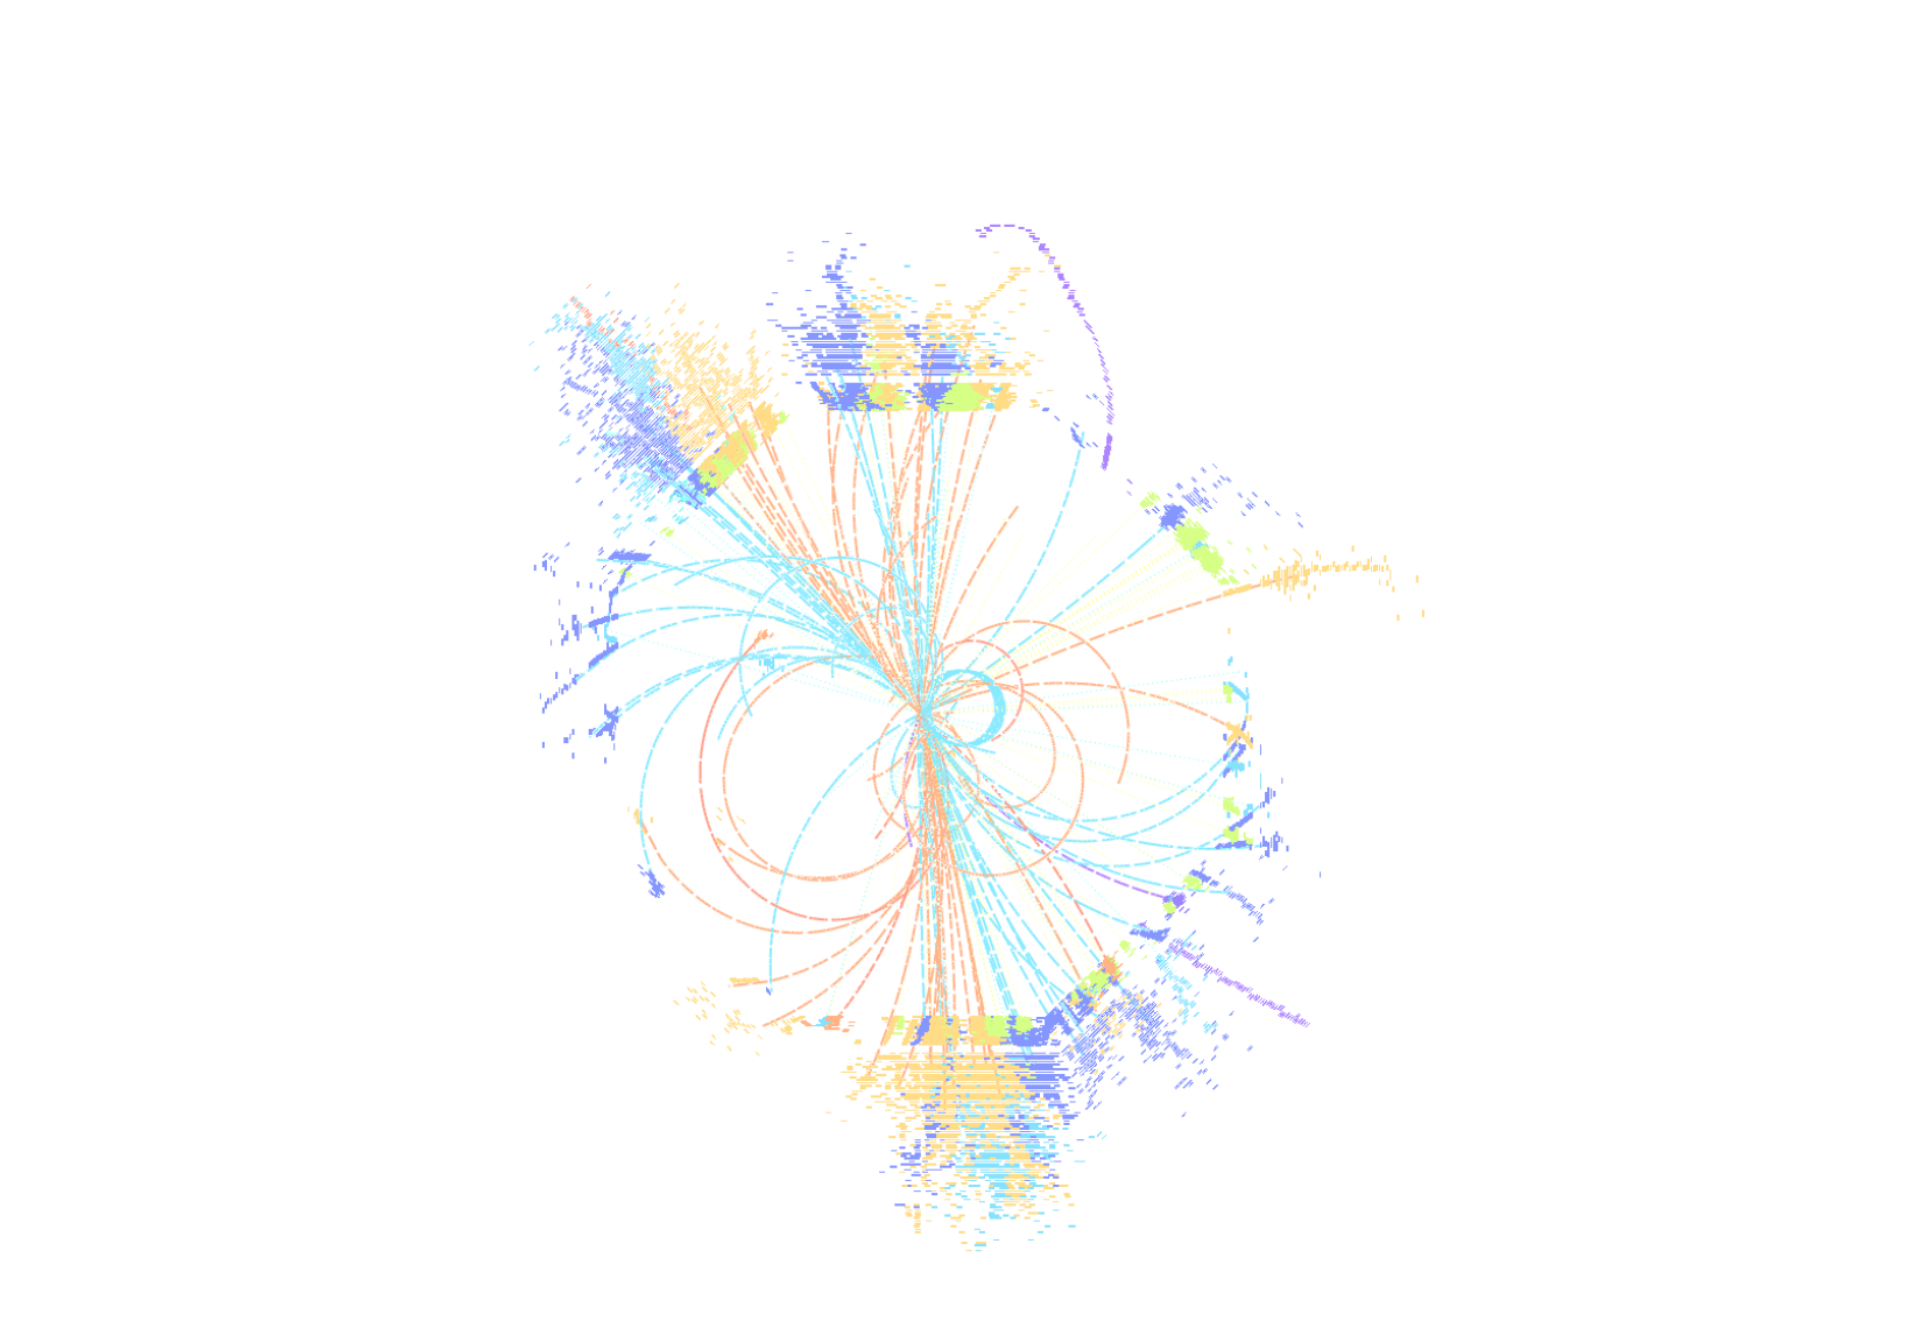
\includegraphics[width=\paperwidth]{background.png}}
	\begin{frame}<beamer>
		\frametitle{Outline}
		\tableofcontents[currentsection,currentsubsection]
	\end{frame}
}
}
\title[]{CLIC Physics \& detectors CDR}
%%\subtitle{Our experience}

\date{\today}

\begin{document}
{
\usebackgroundtemplate{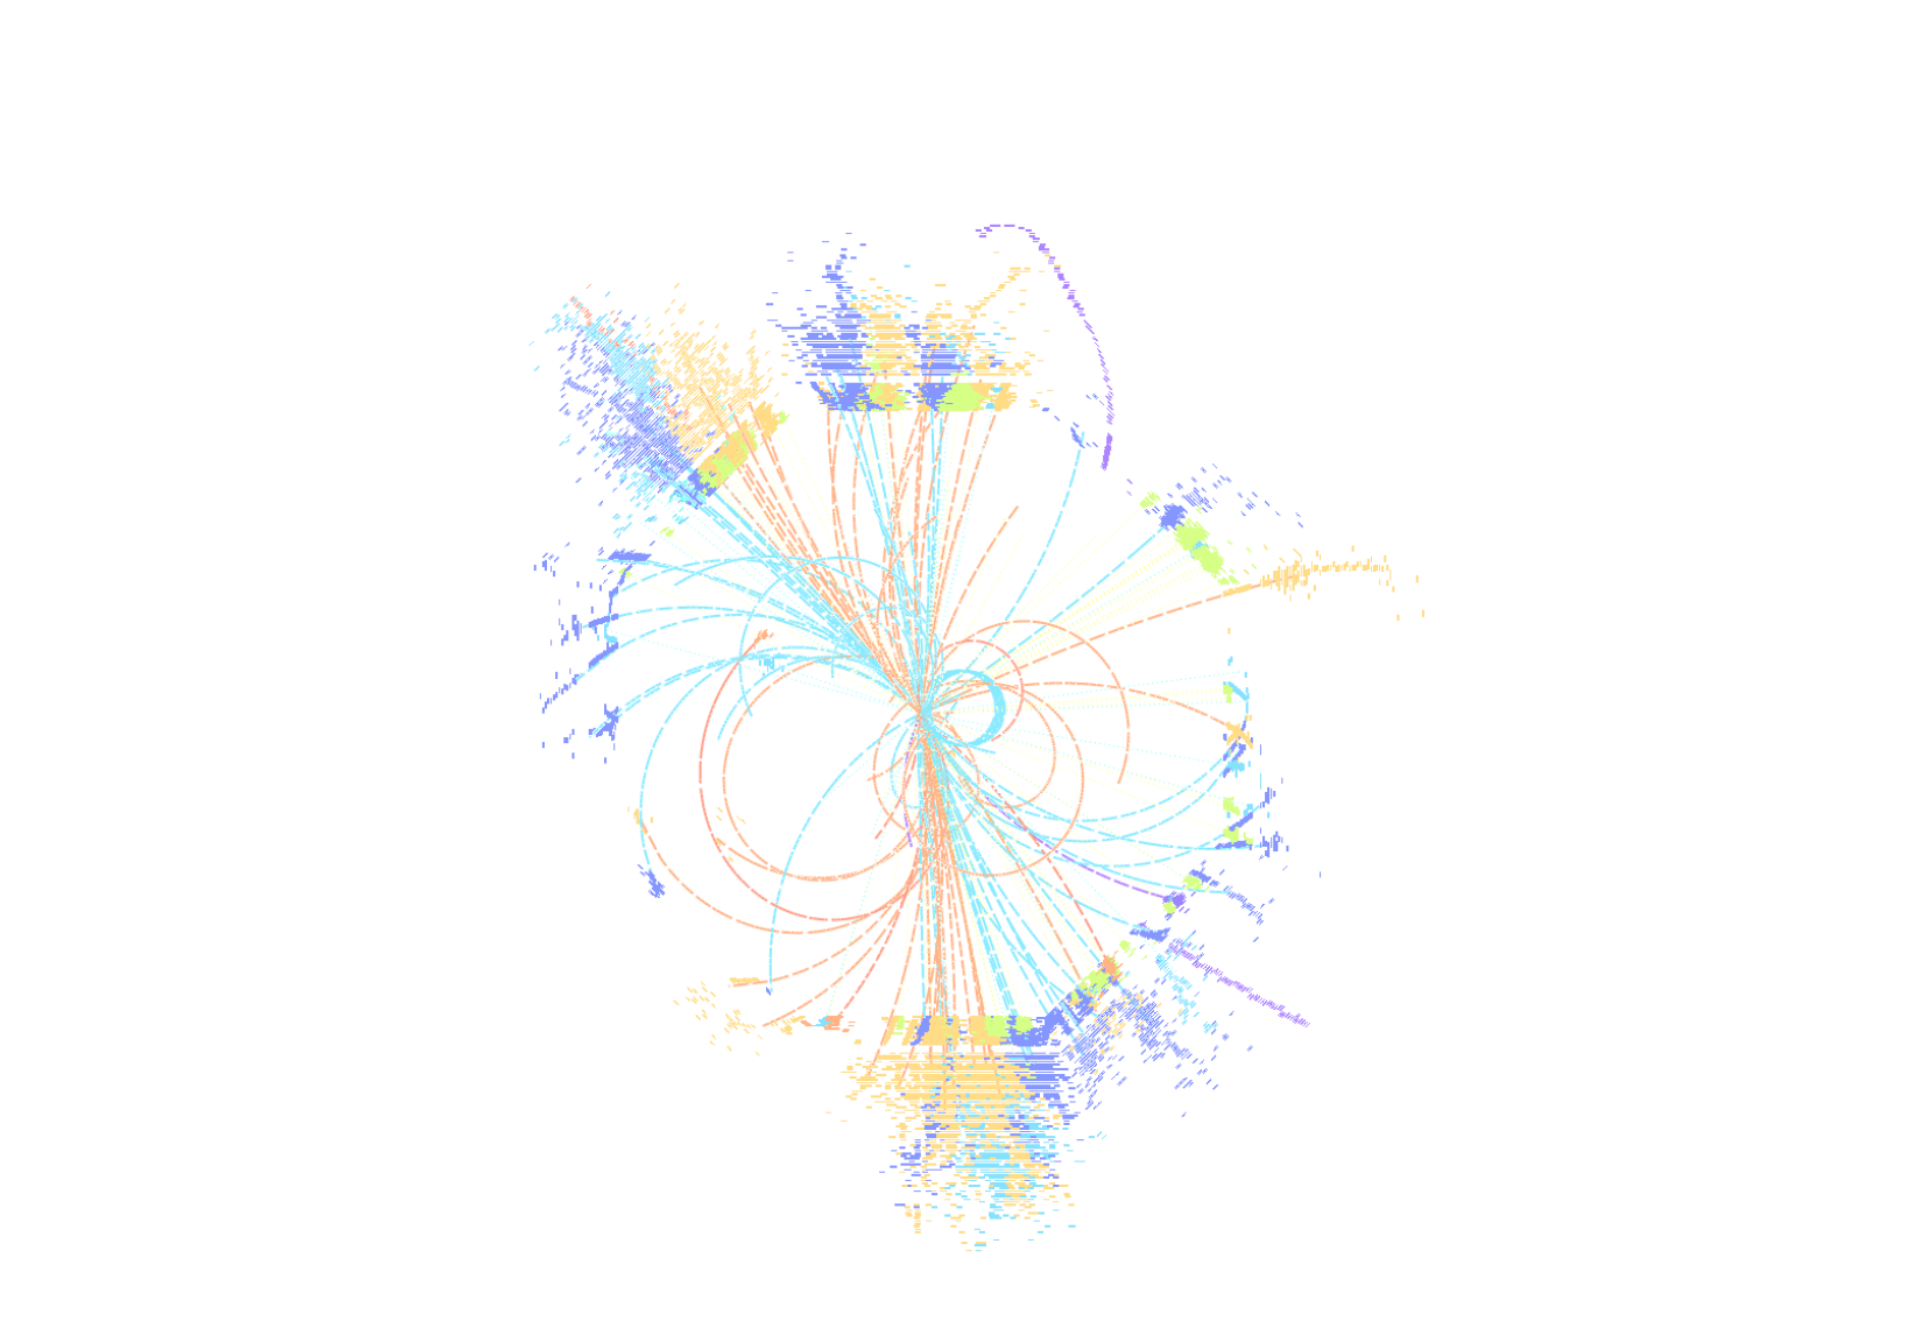
\includegraphics[width=\paperwidth]{background.png}}

\begin{frame}
	\titlepage
\end{frame}

\begin{frame}
\frametitle{Outline}
\tableofcontents
% You might wish to add the option [pausesections]
\end{frame}
}

\section{Physics Motivations}
\begin{frame}
\frametitle{Physics Motivations}
\begin{columns}[c]
\column{6cm}
\begin{itemize} 
  \item 
\end{itemize}
\column{6cm}
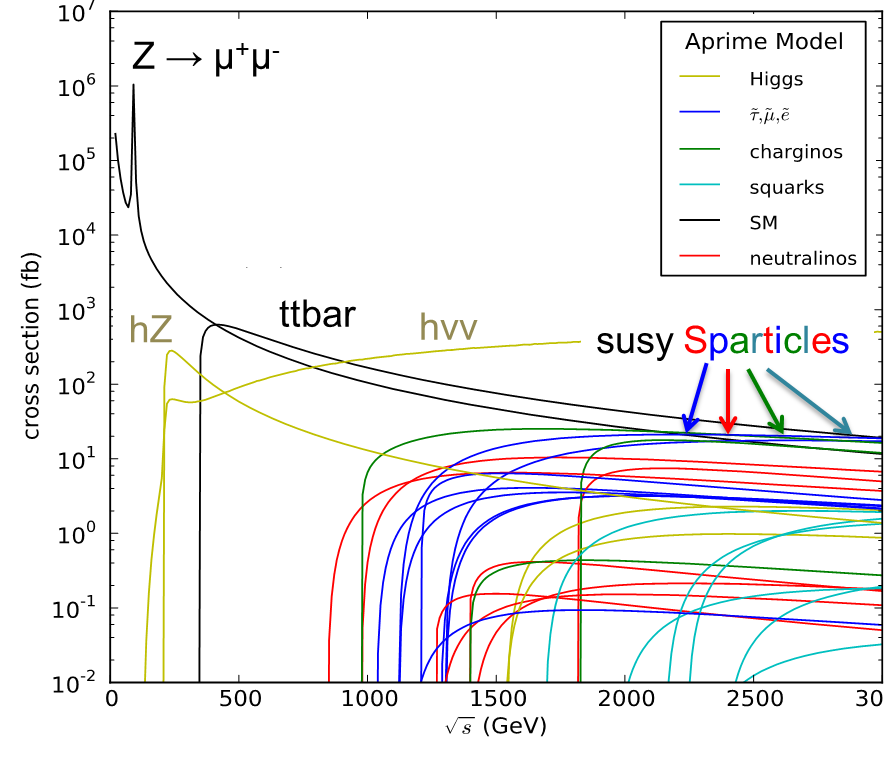
\includegraphics[width=6cm]{models}
\end{columns}
\end{frame}

\begin{frame}
\frametitle{Higgs measurements}
\centering
\begin{columns}[c]
\column{6cm}
\centering
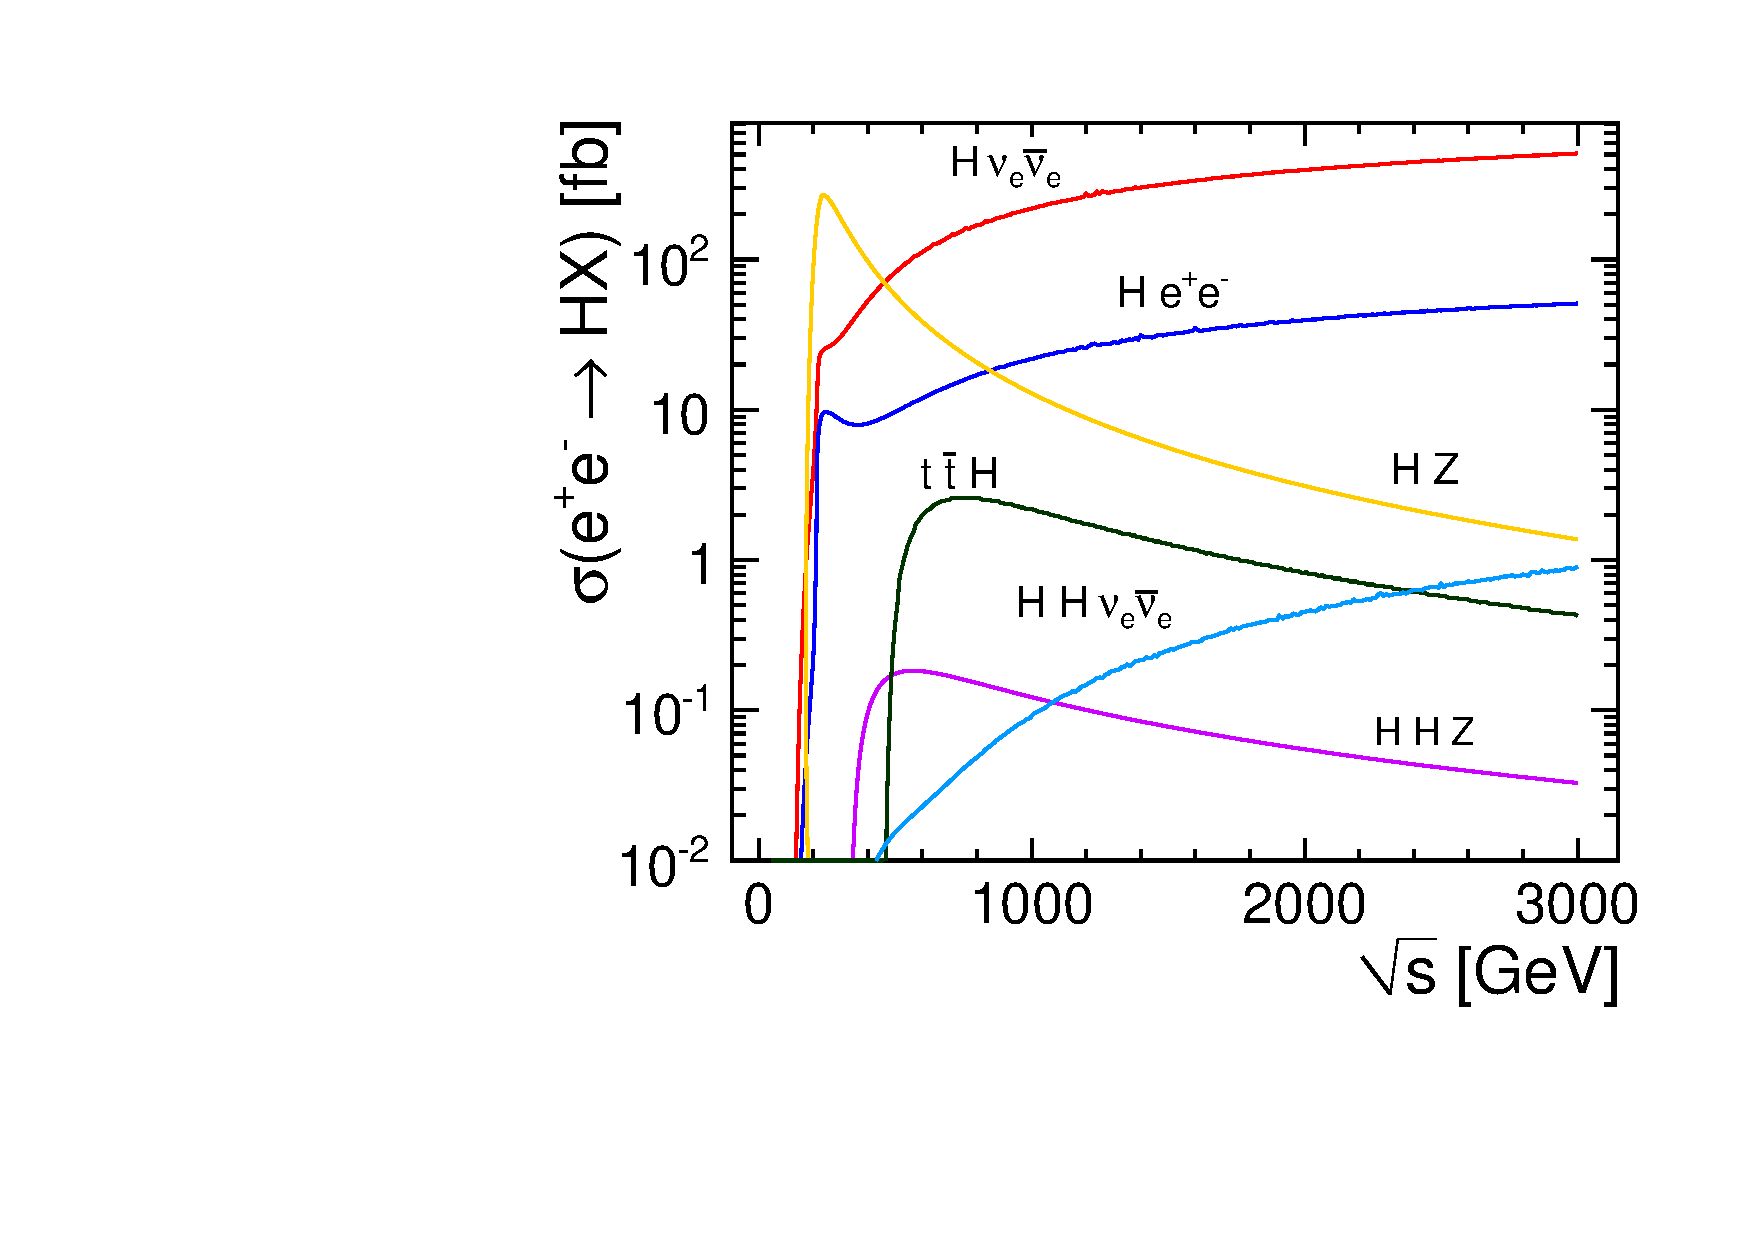
\includegraphics[width=5cm]{xsec_vs_cme}
\column{6cm}
Access to low cross section and small BR processes\\
~\\
\begin{tabular}{ccc}
$\sigma(\Ph\to\mu\mu)$&$\to$ & $\pm15\%$\\
$\sigma(\Ph\to\Pbottom\APbottom)$&$\to$ &$\pm0.2\%$
\end{tabular}
\end{columns}
\begin{columns}[c]
\column{6cm}
\centering
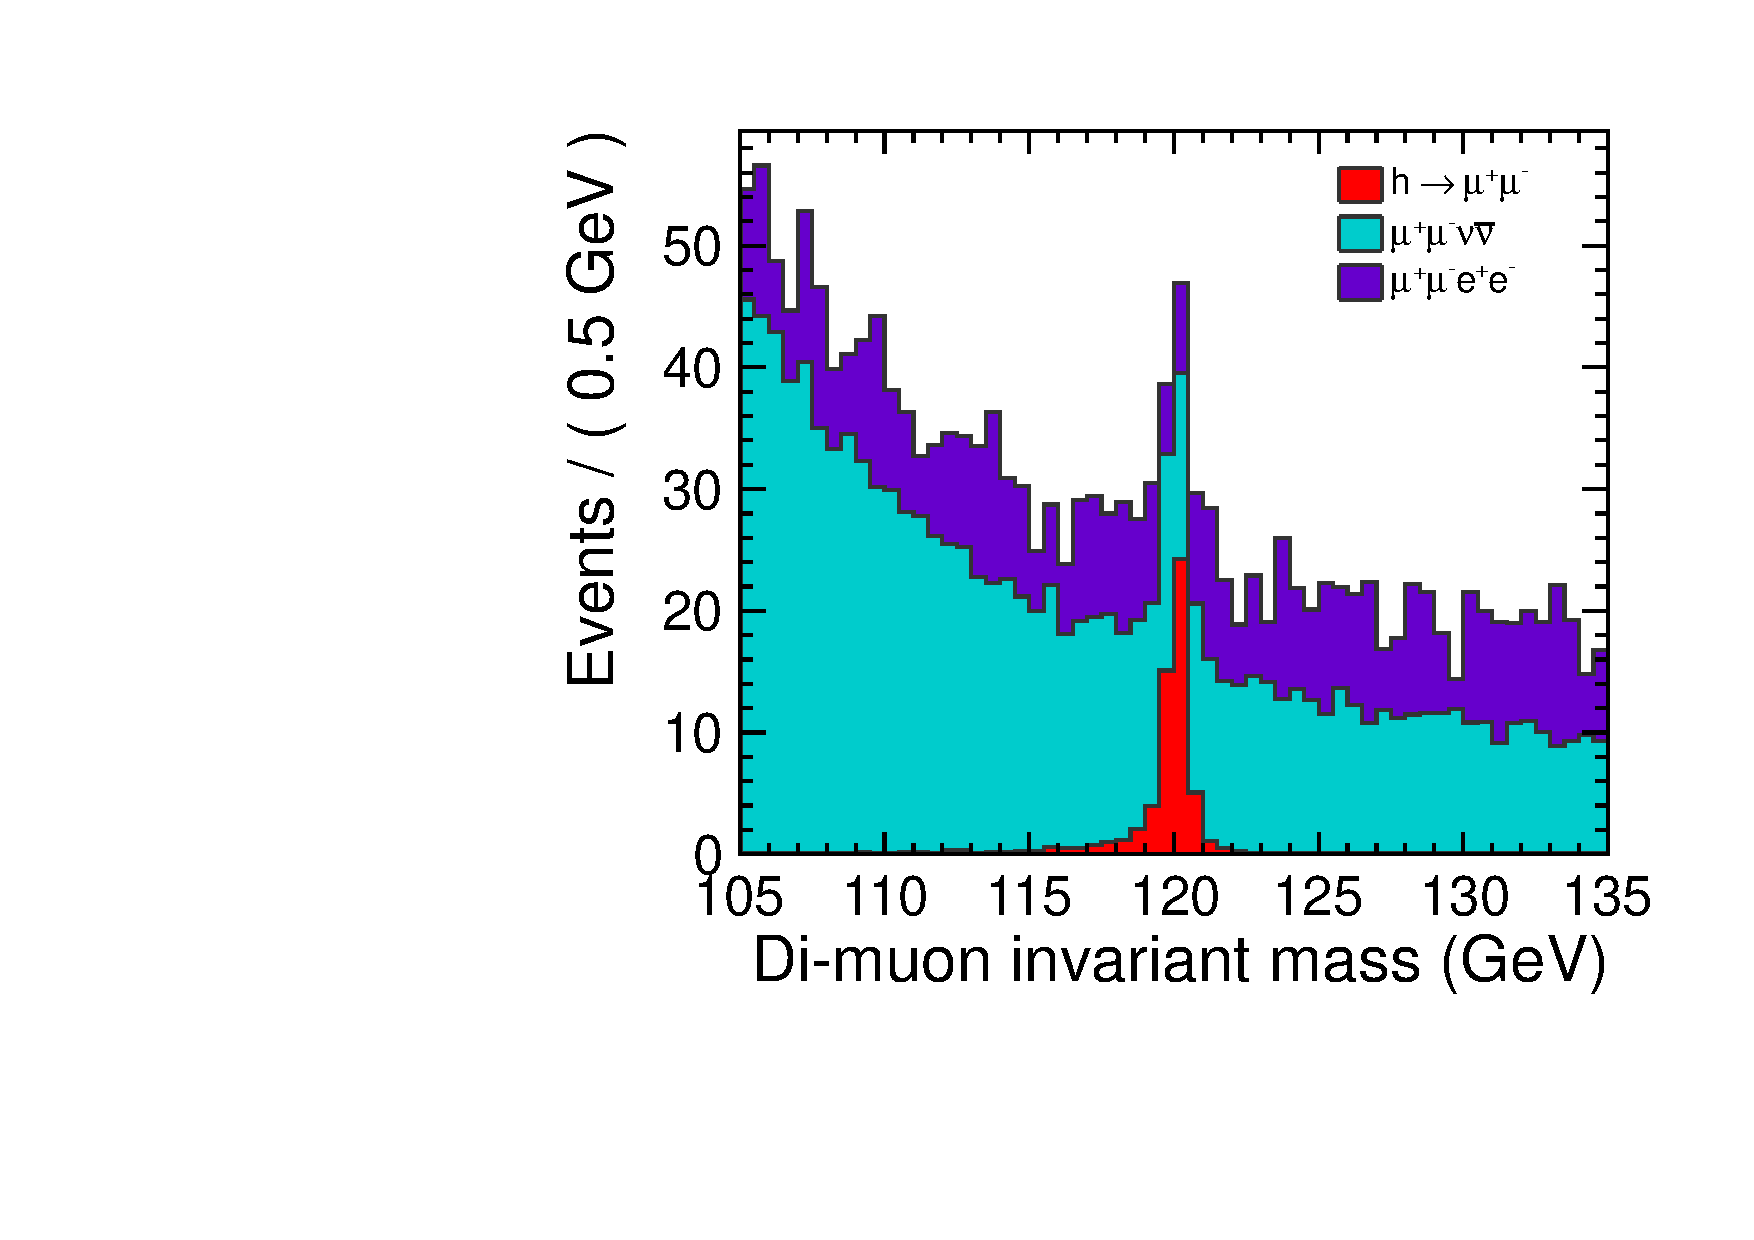
\includegraphics[width=5cm]{ee_h_mumu_mass_mh120GeV}
\column{6cm}
\centering
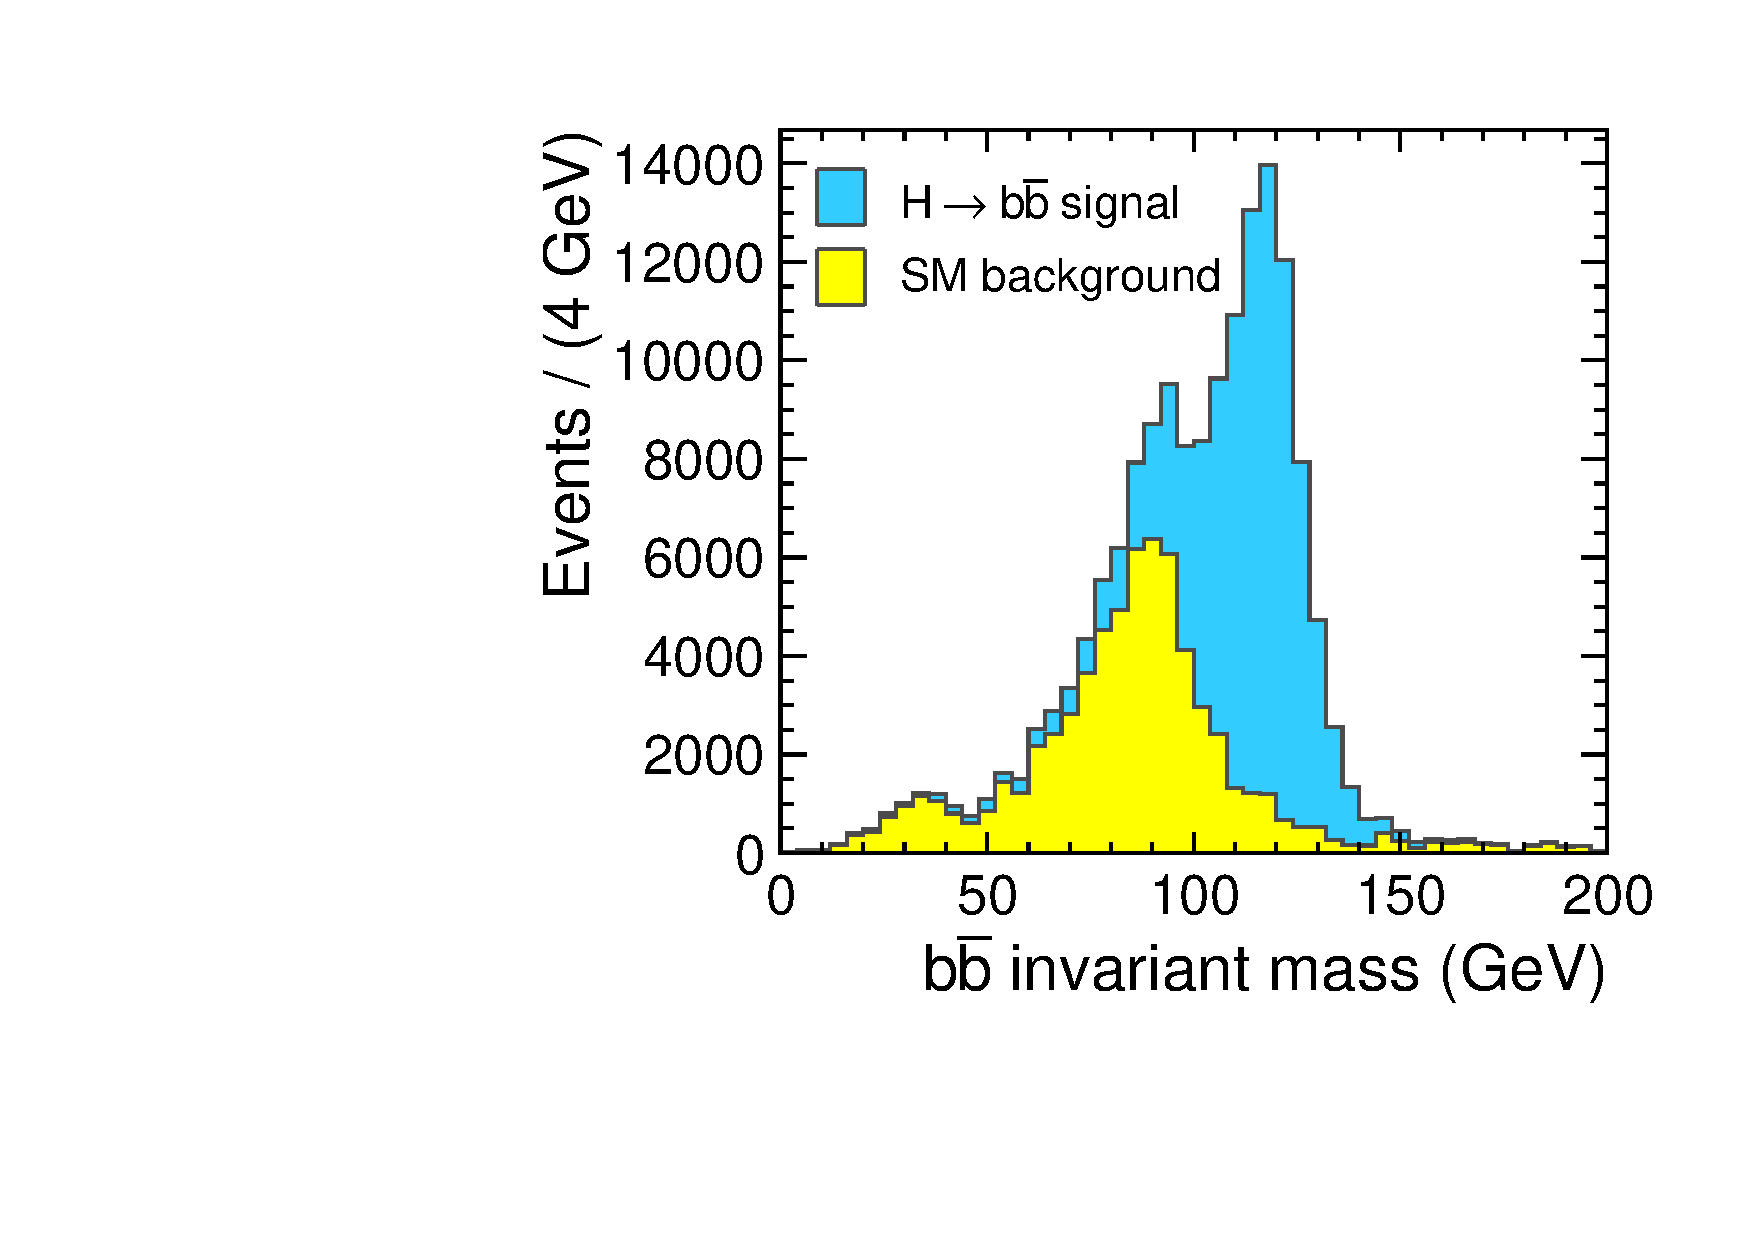
\includegraphics[width=5cm]{ee_h_bb_mass_mh120GeV}
\end{columns}
\end{frame}

\begin{frame}
\frametitle{SUSY}
CLIC resolving power for SUSY breaking models:
\centering
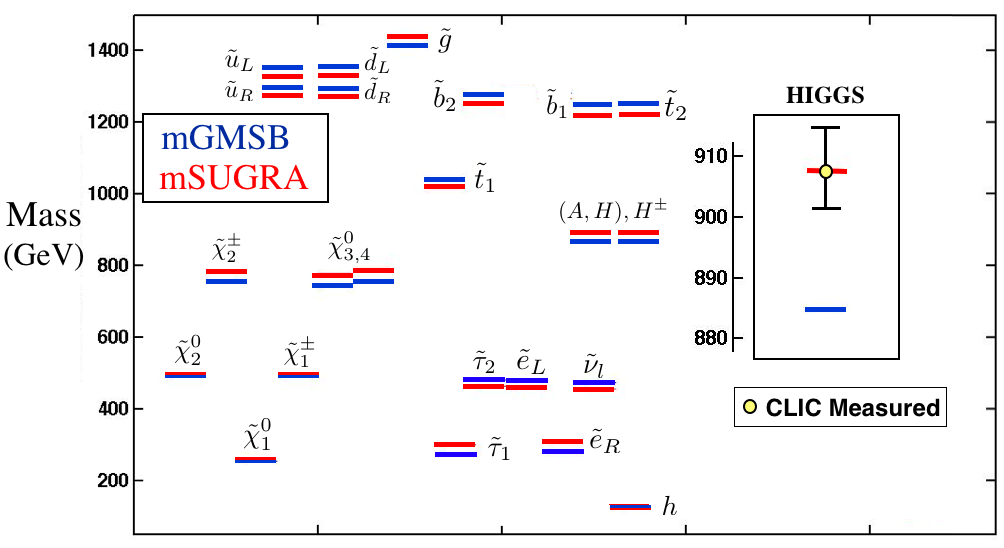
\includegraphics[width=10cm]{GvM}
\end{frame}

\begin{frame}
\frametitle{New physics scenarios}
% \begin{itemize}
%   \item Higgs strong interactions
%   \item Z'
%   \item Contact interactions
%   \item Extra dimensions
% \end{itemize}
\begin{center}
{\scriptsize
 \begin{tabular}{ ccccc }
    \toprule
 New particle &     LHC14 & SLHC & LC800 & CLIC3\\
 Luminosity & $100\textrm{fb}^{-1}$ & $1\textrm{ab}^{-1}$&
 $500\textrm{fb}^{-1}$& $1\textrm{ab}^{-1}$\\
\midrule
squarks [TeV] &   2.5 & 3 & 0.4 & 1.5 \\
sleptons [TeV] &   0.3 & - & 0.4 & 1.5 \\ 
$\textrm{Z}'$ ({\tiny SM ~couplings}) [TeV]  &  5 & 7 & 8 & 20   \\ 
%\Zprime ({\tiny SM~couplings})  &     5& 6  & 8 & 22 \\
%$q*$      &    6.5 & 7.5 & 0.8 & 3 \\
%$l*$       &   3.4 & - & 0.8 & 3 \\
2 extra dims $M_D$ [TeV]  &    9 & 12 & 5-8.5 & 20-30 \\
%$W_L W_L$      &  3.4sig& >3.4sig& -& 70sig\\
TGC (95\%)  ({\tiny \rm $\lambda_{\gamma} $~coupling}) &   0.001& 0.0006& 0.0004& 0.0001 \\
$\mu$ contact scale [TeV] &  15& - & 20 & 60 \\
Higgs compos. scale [TeV] & 5-7 & 9-12 & 30 & 30\\
    \bottomrule
  \end{tabular}
  }
 \end{center}
\end{frame}

\section[CLIC]{A few words on the CLIC machine and beam} 
\begin{frame}
\frametitle{A particular beam structure}
\begin{itemize}
  \item CLIC: trains at 50Hz, 1 train is 312 bunches, 0.5ns apart: \alert{156ns
  for full bunch train}
  \item ILC: trains at 5Hz, 1 train is 1300 bunches, 700ns apart
\end{itemize}
\centering
\begin{tabular}{lcc}
 & ILC 0.5TeV & CLIC 3TeV\\
 \hline
L [$\textrm{cm}^{-2}\,\textrm{s}^{-1}$] & $2\times 10^{34}$&$5.9\times 10^{34}$ \\
\hline
Crossing angle & 14mrad & 20mrad\\
\hline
BX separation & 700ns & \alert{0.5ns}\\
\hline
Nb $\gamma\gamma\to\textrm{had}$/BX & 0.2 & \alert{3.2}\\
\hline
Nb incoherant pairs/BX & $1\times 10^5$ & \alert{$3\times10^5$}\\
\hline
\end{tabular}
~\\
~\\
\alert{Very large machine induced background rate!}
\end{frame}

%\begin{frame}
%\frametitle{Running conditions}
%overlay, pairs
%\end{frame}

\section{The detectors concepts}
\begin{frame}
\frametitle{The detector requirements}
\begin{itemize}
  \item Trigger less readout of full train: time stamping, multi-hit capacity,
  filtering algorithms during reconstruction
  \item High resolution pixel detector for displaced vertices identification:\\
  {\scriptsize
  \begin{tabular}{lc}
  p = 1 Gev & $\sigma_{d0}\sim20\mu m$\\
  p = 100 GeV & $\sigma_{d0}\sim5\mu m$
  \end{tabular}
  }~\\ ~\\
  \item Momentum resolution:\\
  {\scriptsize 
  $\sigma(p_{\textrm{T}})/p_{\textrm{T}}^2\sim 10^{-5}\textrm{GeV}^{-1}$
   }~\\ ~\\
  \item Good jet-energy resolution (W/Z separation)\\
  {\scriptsize 
$\sigma(E_j)/E_j = 3.5\%-5\%$ for $E_j = 50\textrm{GeV}-1\textrm{TeV}$
  }~\\ ~\\
  
\end{itemize}
\end{frame}
\begin{frame}
\frametitle{The CLIC detectors}
Main differences with ILC concepts:
\begin{itemize}
  \item Denser barrel HCAL, using tungsten, 7.5$\lambda_{\textrm{I}}$
  \item Redesign of the vertex detector and forward region to account for the
  higher rates
\end{itemize}
\begin{columns}[c]
\column{6cm}
\centering
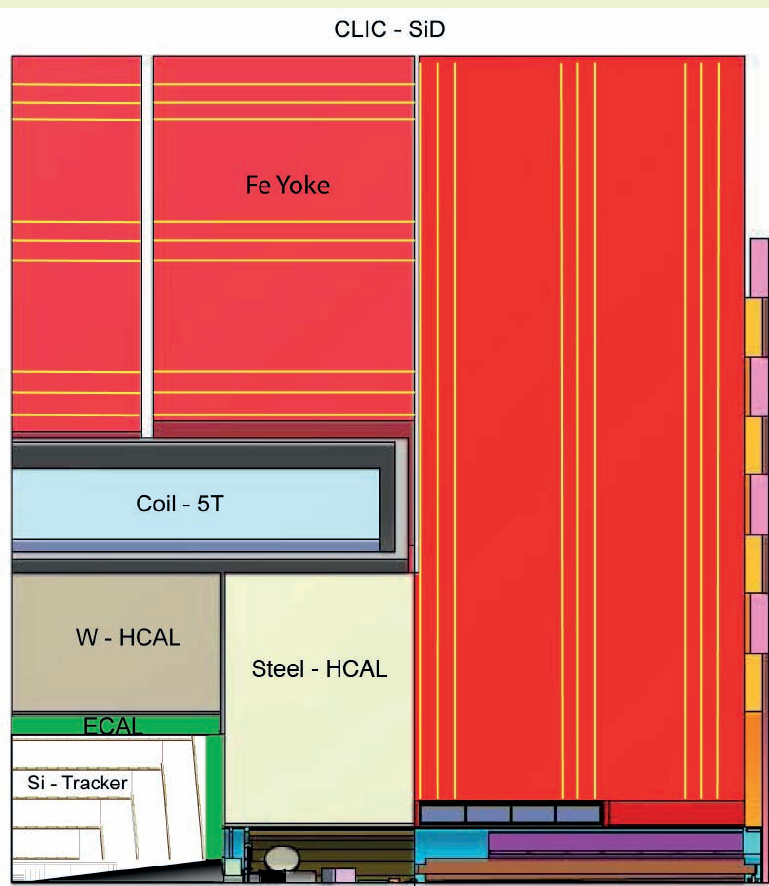
\includegraphics[width=5cm]{CLIC_SiD_xz.pdf}
\column{6cm}
\centering
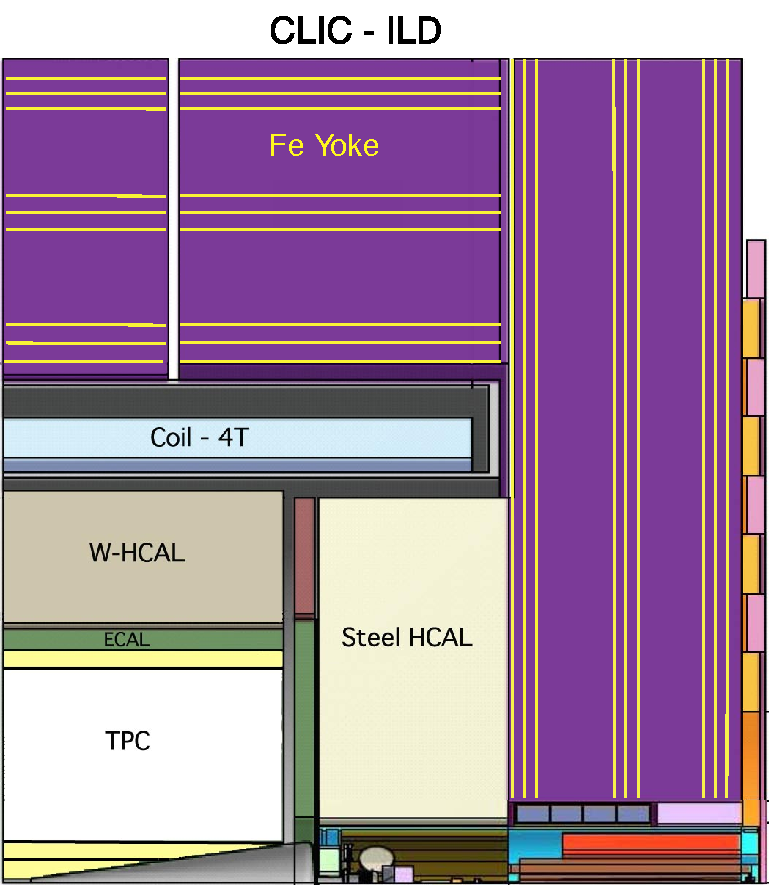
\includegraphics[width=5cm]{CLIC_ILD_xz.pdf}
\end{columns}
\end{frame}

\section[Bkg suppression]{Background suppression}
\begin{frame}
\frametitle{Background properties}
Main problematic background: $\gamma\gamma\to\textrm{hadrons}$
\begin{columns}[c]
\column{6cm}
\centering
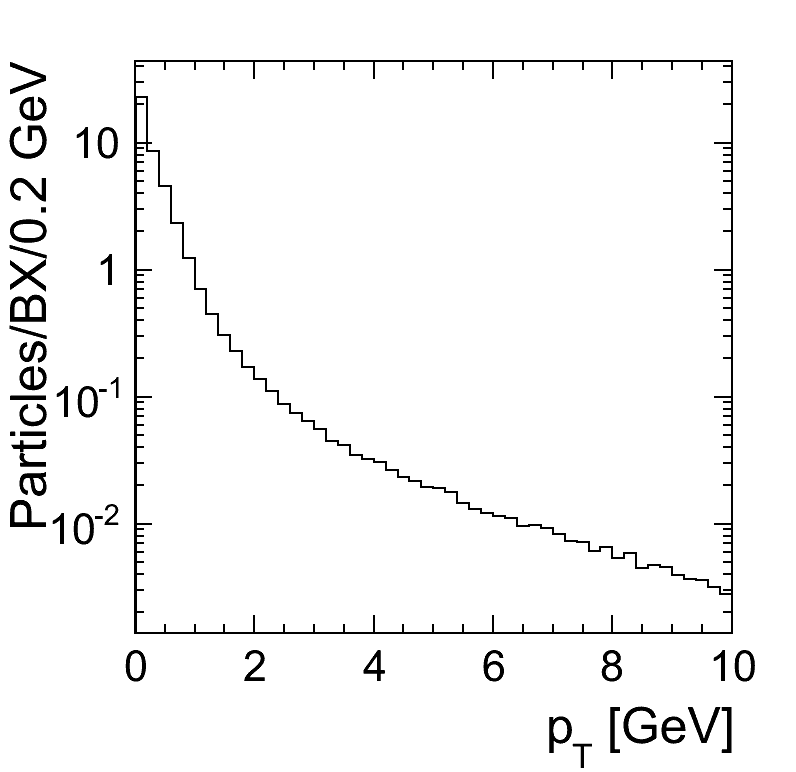
\includegraphics[width=4cm]{ggPT}\\
$\theta>8^\circ$
\column{6cm}
Entire bunch train (312BX):
\begin{itemize}
  \item 5000 tracks $\to$ total track momentum: \alert{7.3TeV}
  \item Total calorimetric energy (ECAL+HCAL): \alert{19TeV}
\end{itemize}
Mostly low $p_{\textrm{T}}$
\end{columns}
\end{frame}
\begin{frame}
\frametitle{Background suppression: timing}
\begin{columns}[c]
\column{5cm}
\centering
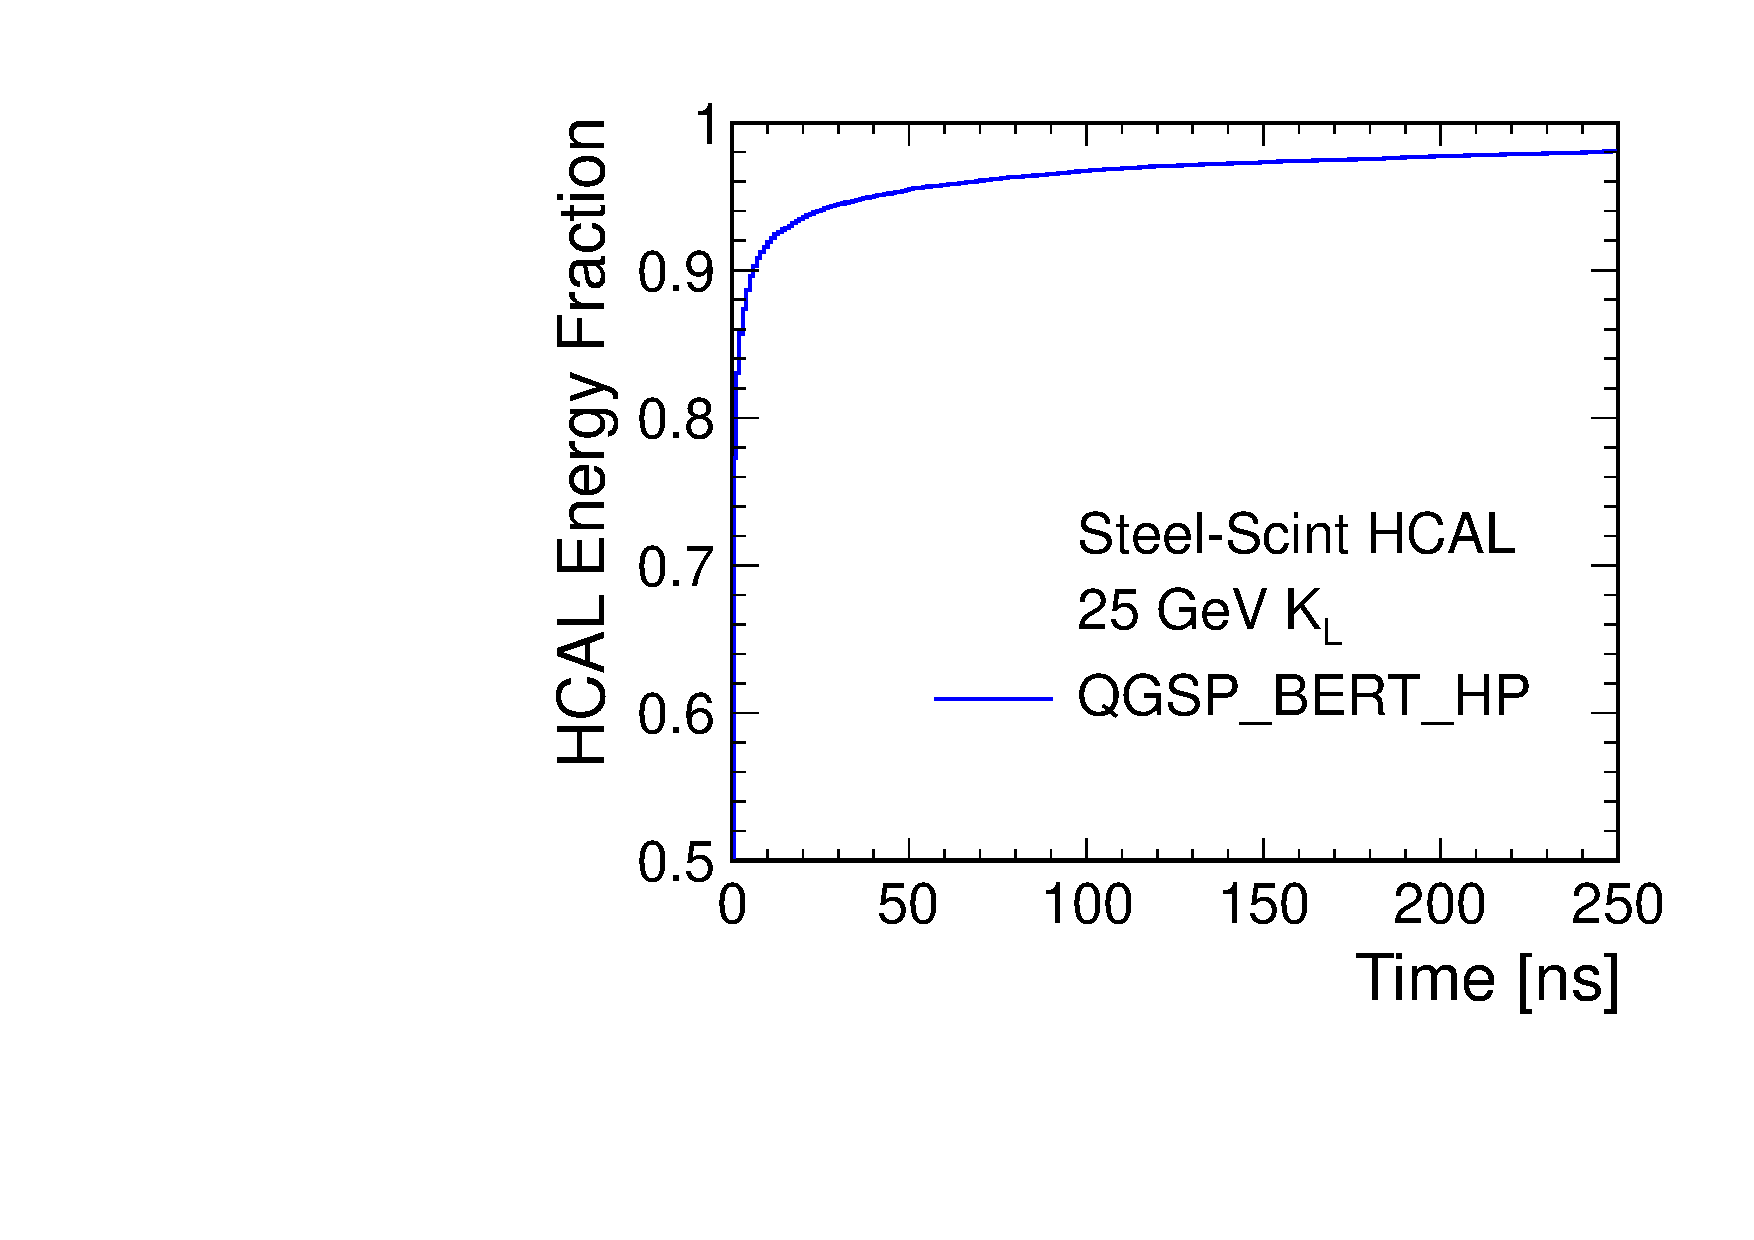
\includegraphics[width=5cm]{hcalTimingSteel.pdf}
\column{5cm}
\centering
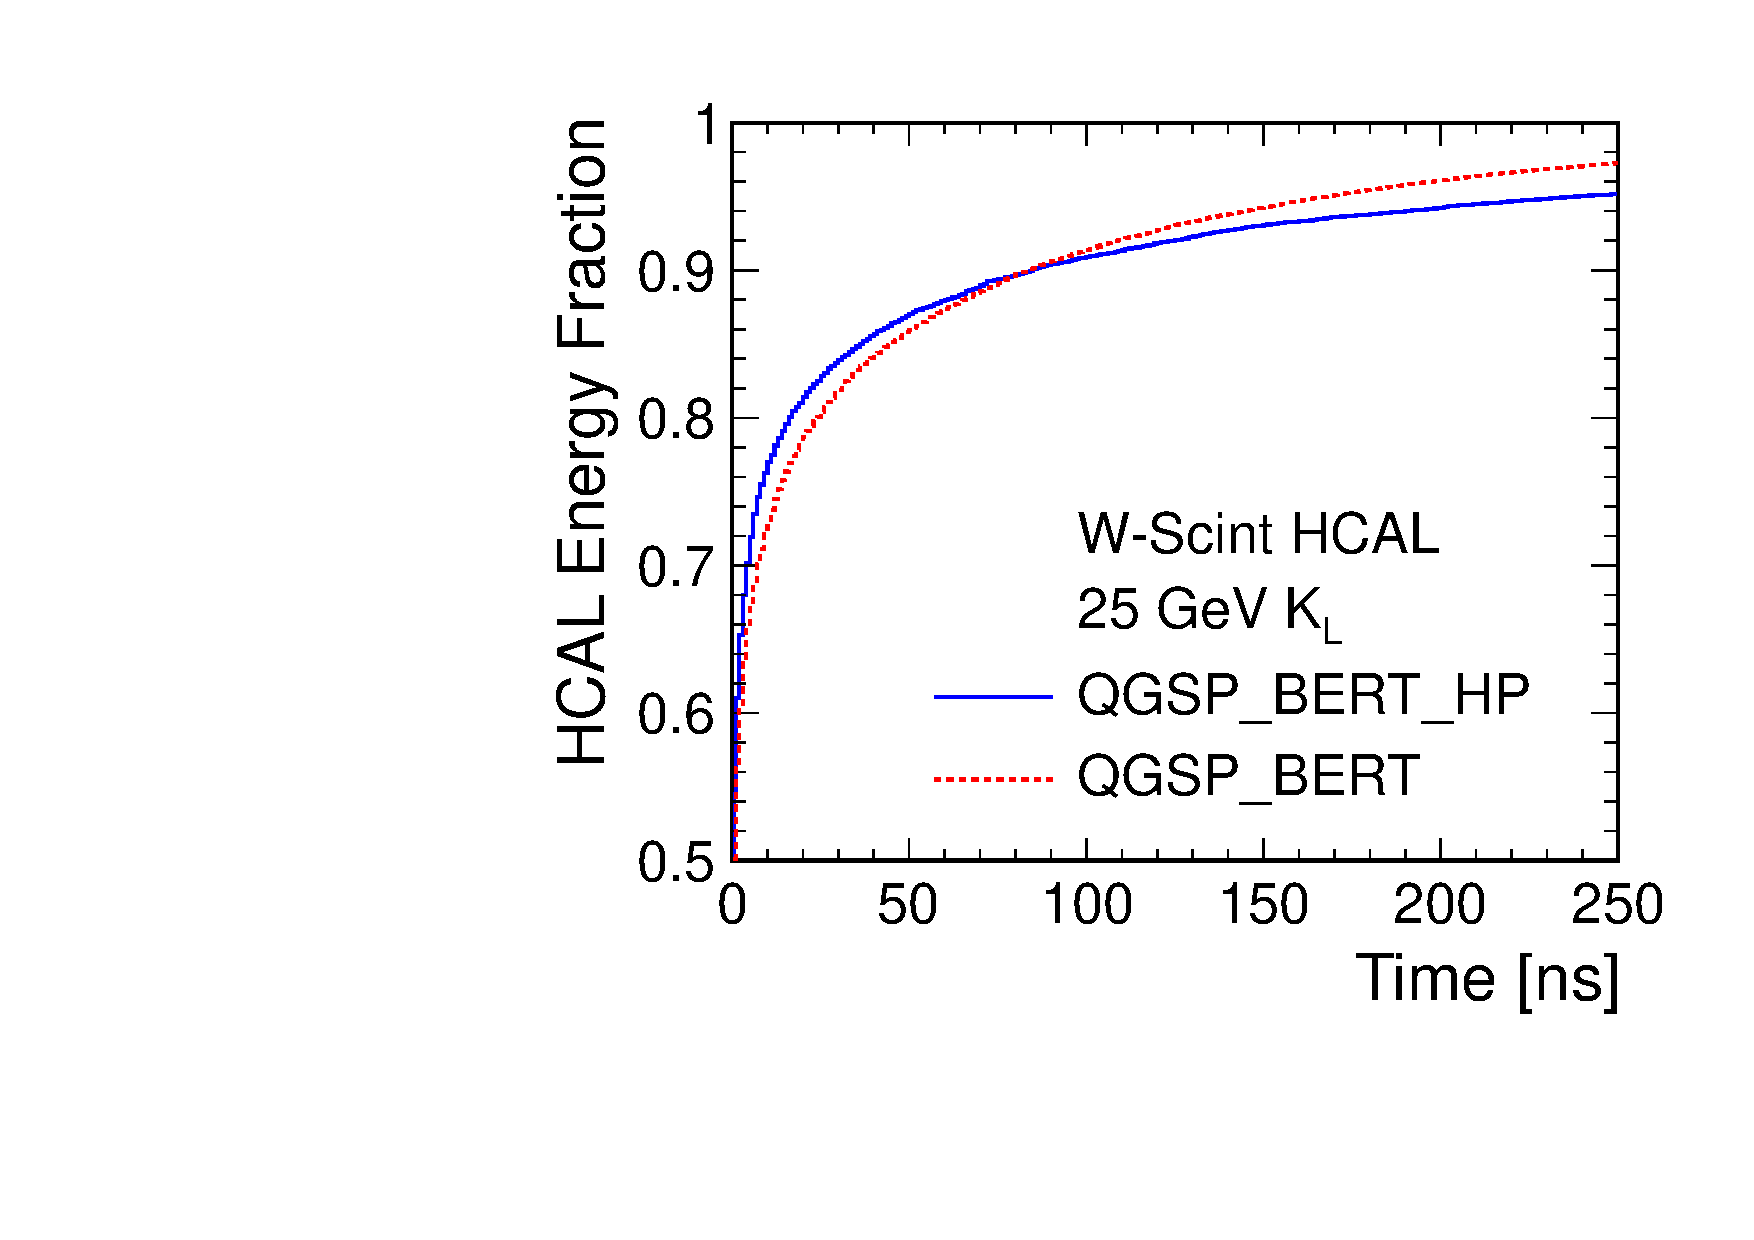
\includegraphics[width=5cm]{hcalTimingTungsten.pdf}
\end{columns}
\begin{center}
\begin{tabular}{lrr}
Subdetector &Reco. window &hit resolution\\
ECAL &10 ns &1 ns\\
HCAL Endcaps &10 ns &1 ns\\
HCAL Barrel &100 ns &1 ns\\
Silicon Detectors &10 ns &$10/\sqrt{12}$ ns
\end{tabular}
\end{center}
\end{frame}
\begin{frame}
\frametitle{Background suppression: jet finder}
$\Pep\Pem\to\PSq_R\PaSq_R\to\Pquark\APquark\PSgxz_1 \PSgxz_1$: 2 jets $+$
missing energy\\ ~\\
\begin{columns}[c]
\column{6cm}
Durham $k_{\textrm{T}}$ \`a la LEP:\\
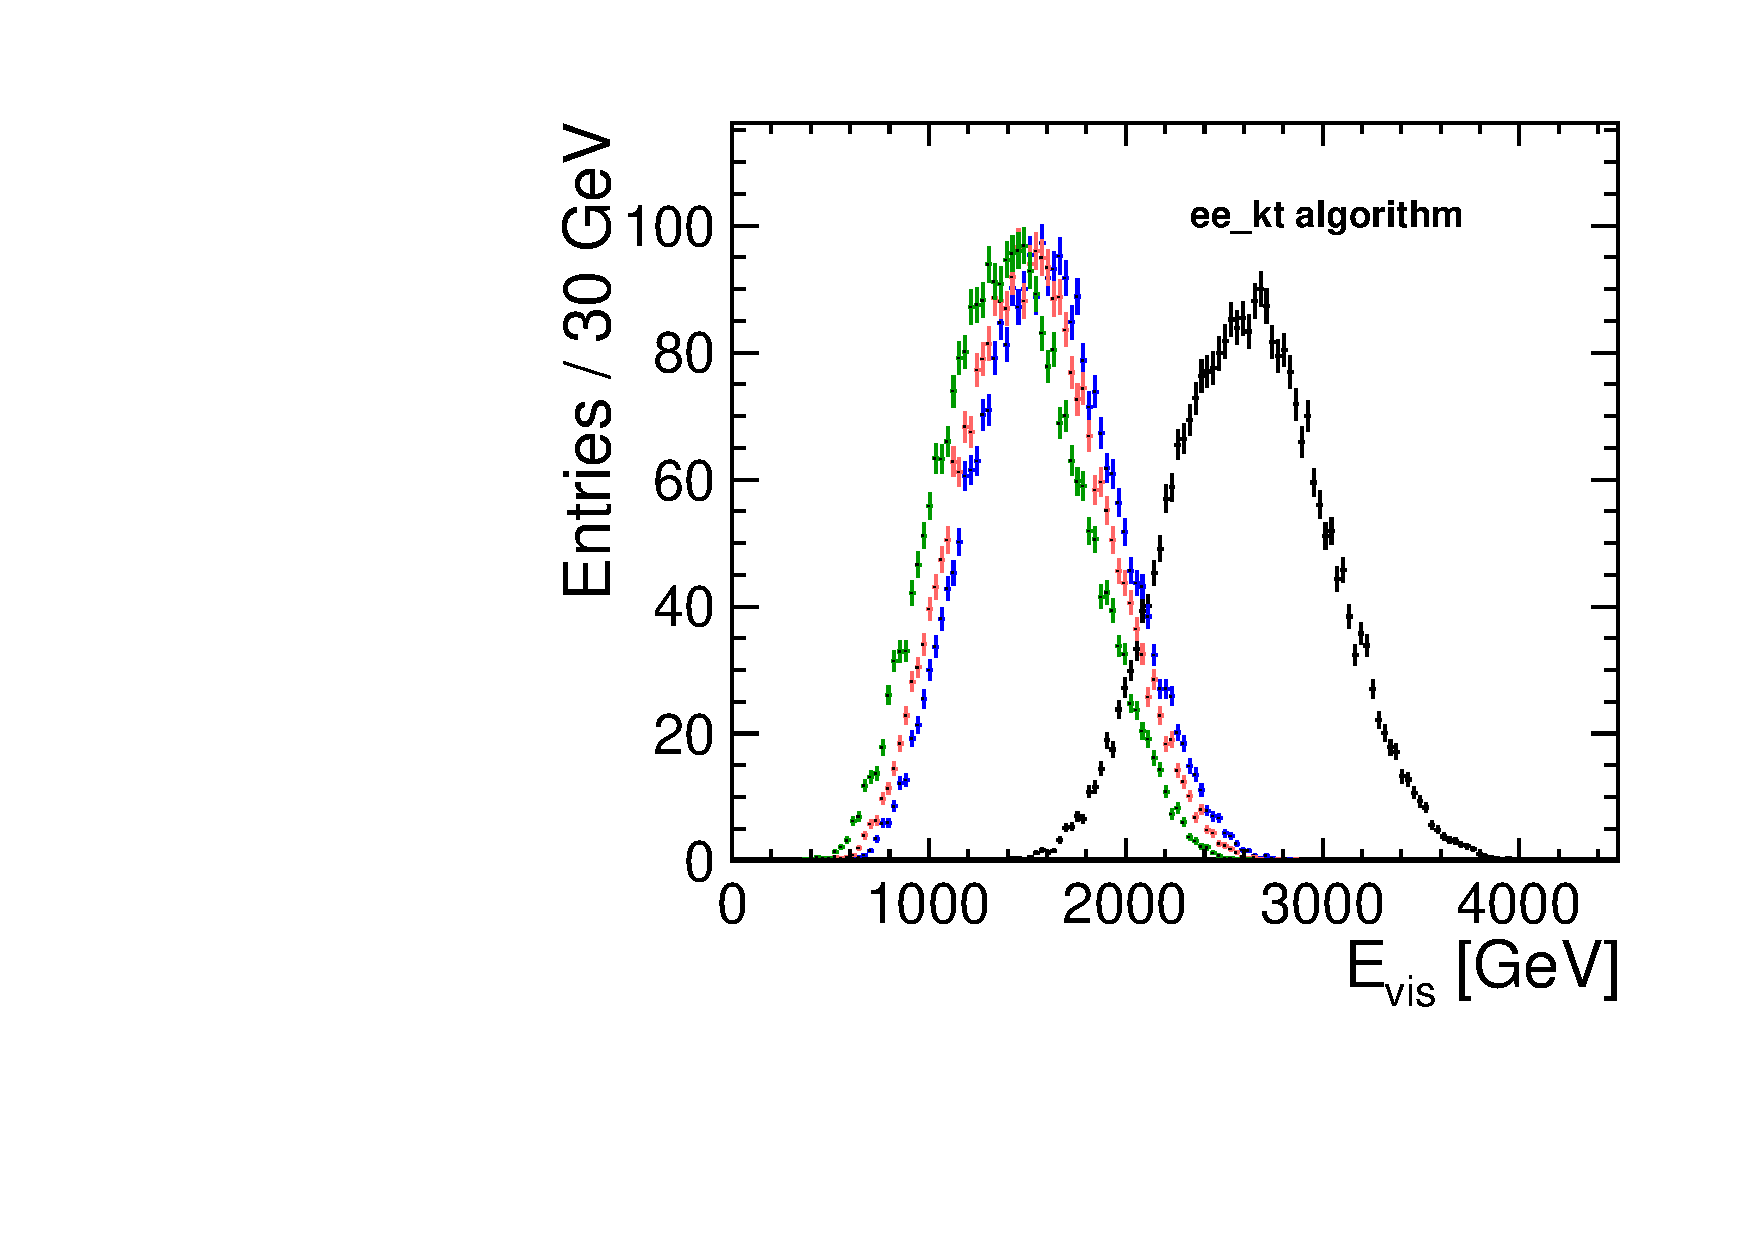
\includegraphics[width=6cm]{JetFinding_compare_E_vis__FJ_ee_kt_algorithm_ExclusiveNJets_2.pdf}\\
\column{6cm}
Hadron collider $k_{\textrm{T}}$:\\
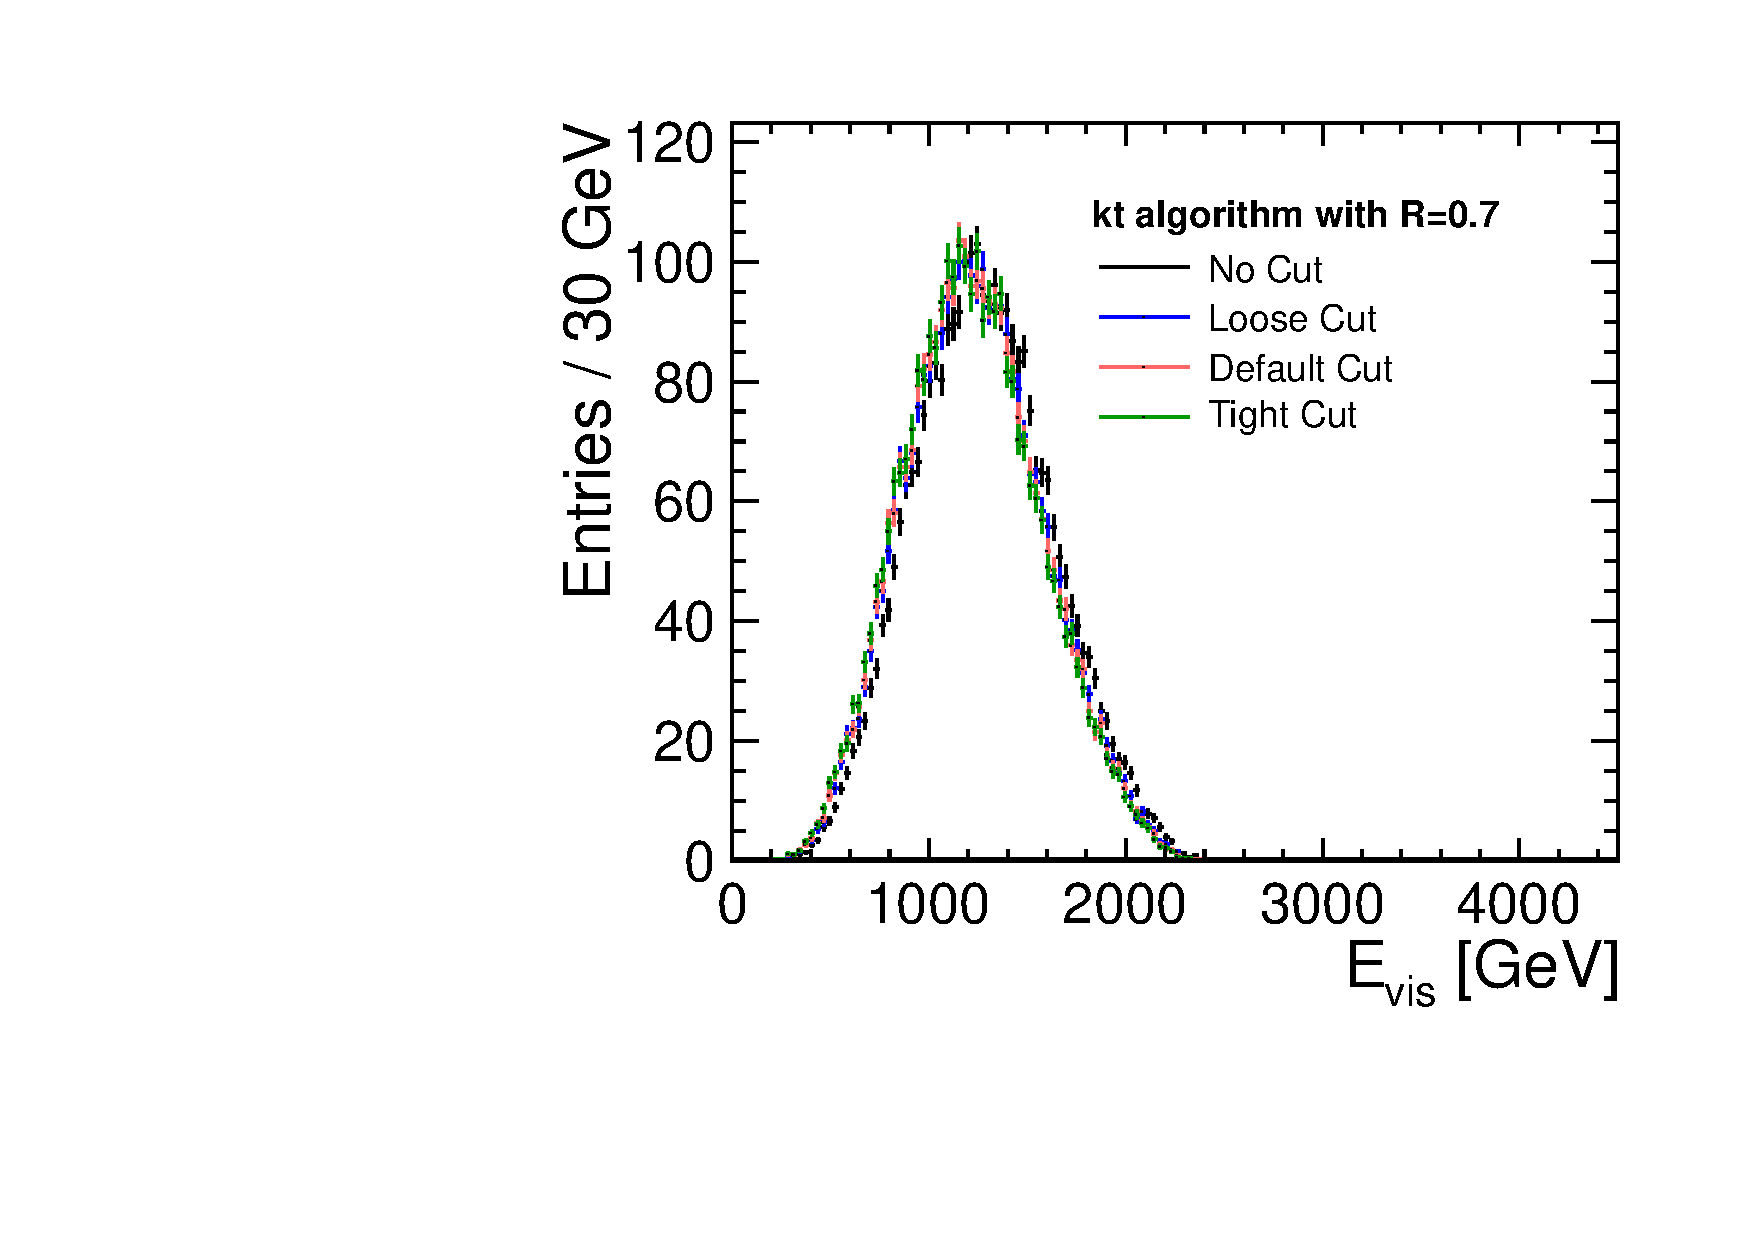
\includegraphics[width=6cm]{JetFinding_compare_E_vis__FJ_kt_algorithm_0_7_ExclusiveNJets_2.pdf}\\
\end{columns}
\begin{columns}
\column{6cm}
{\scriptsize
\begin{itemize}
  \item All particle clustered
  \item Timing cuts effective
\end{itemize}
}
\column{6cm}
{\scriptsize
\begin{itemize}
  \item Much of Bkg clustered with beam axis
  \item Timing cuts do less work
  \item Impact depends on event topology
\end{itemize}
}
\end{columns}
\end{frame}
\begin{frame}
\frametitle{Background suppression}
E.g. $\Pep\Pem\to\PH\PH\to\Ptop\APbottom\Pbottom\APtop$:
\begin{columns}[c]
\column{6cm}
\centering
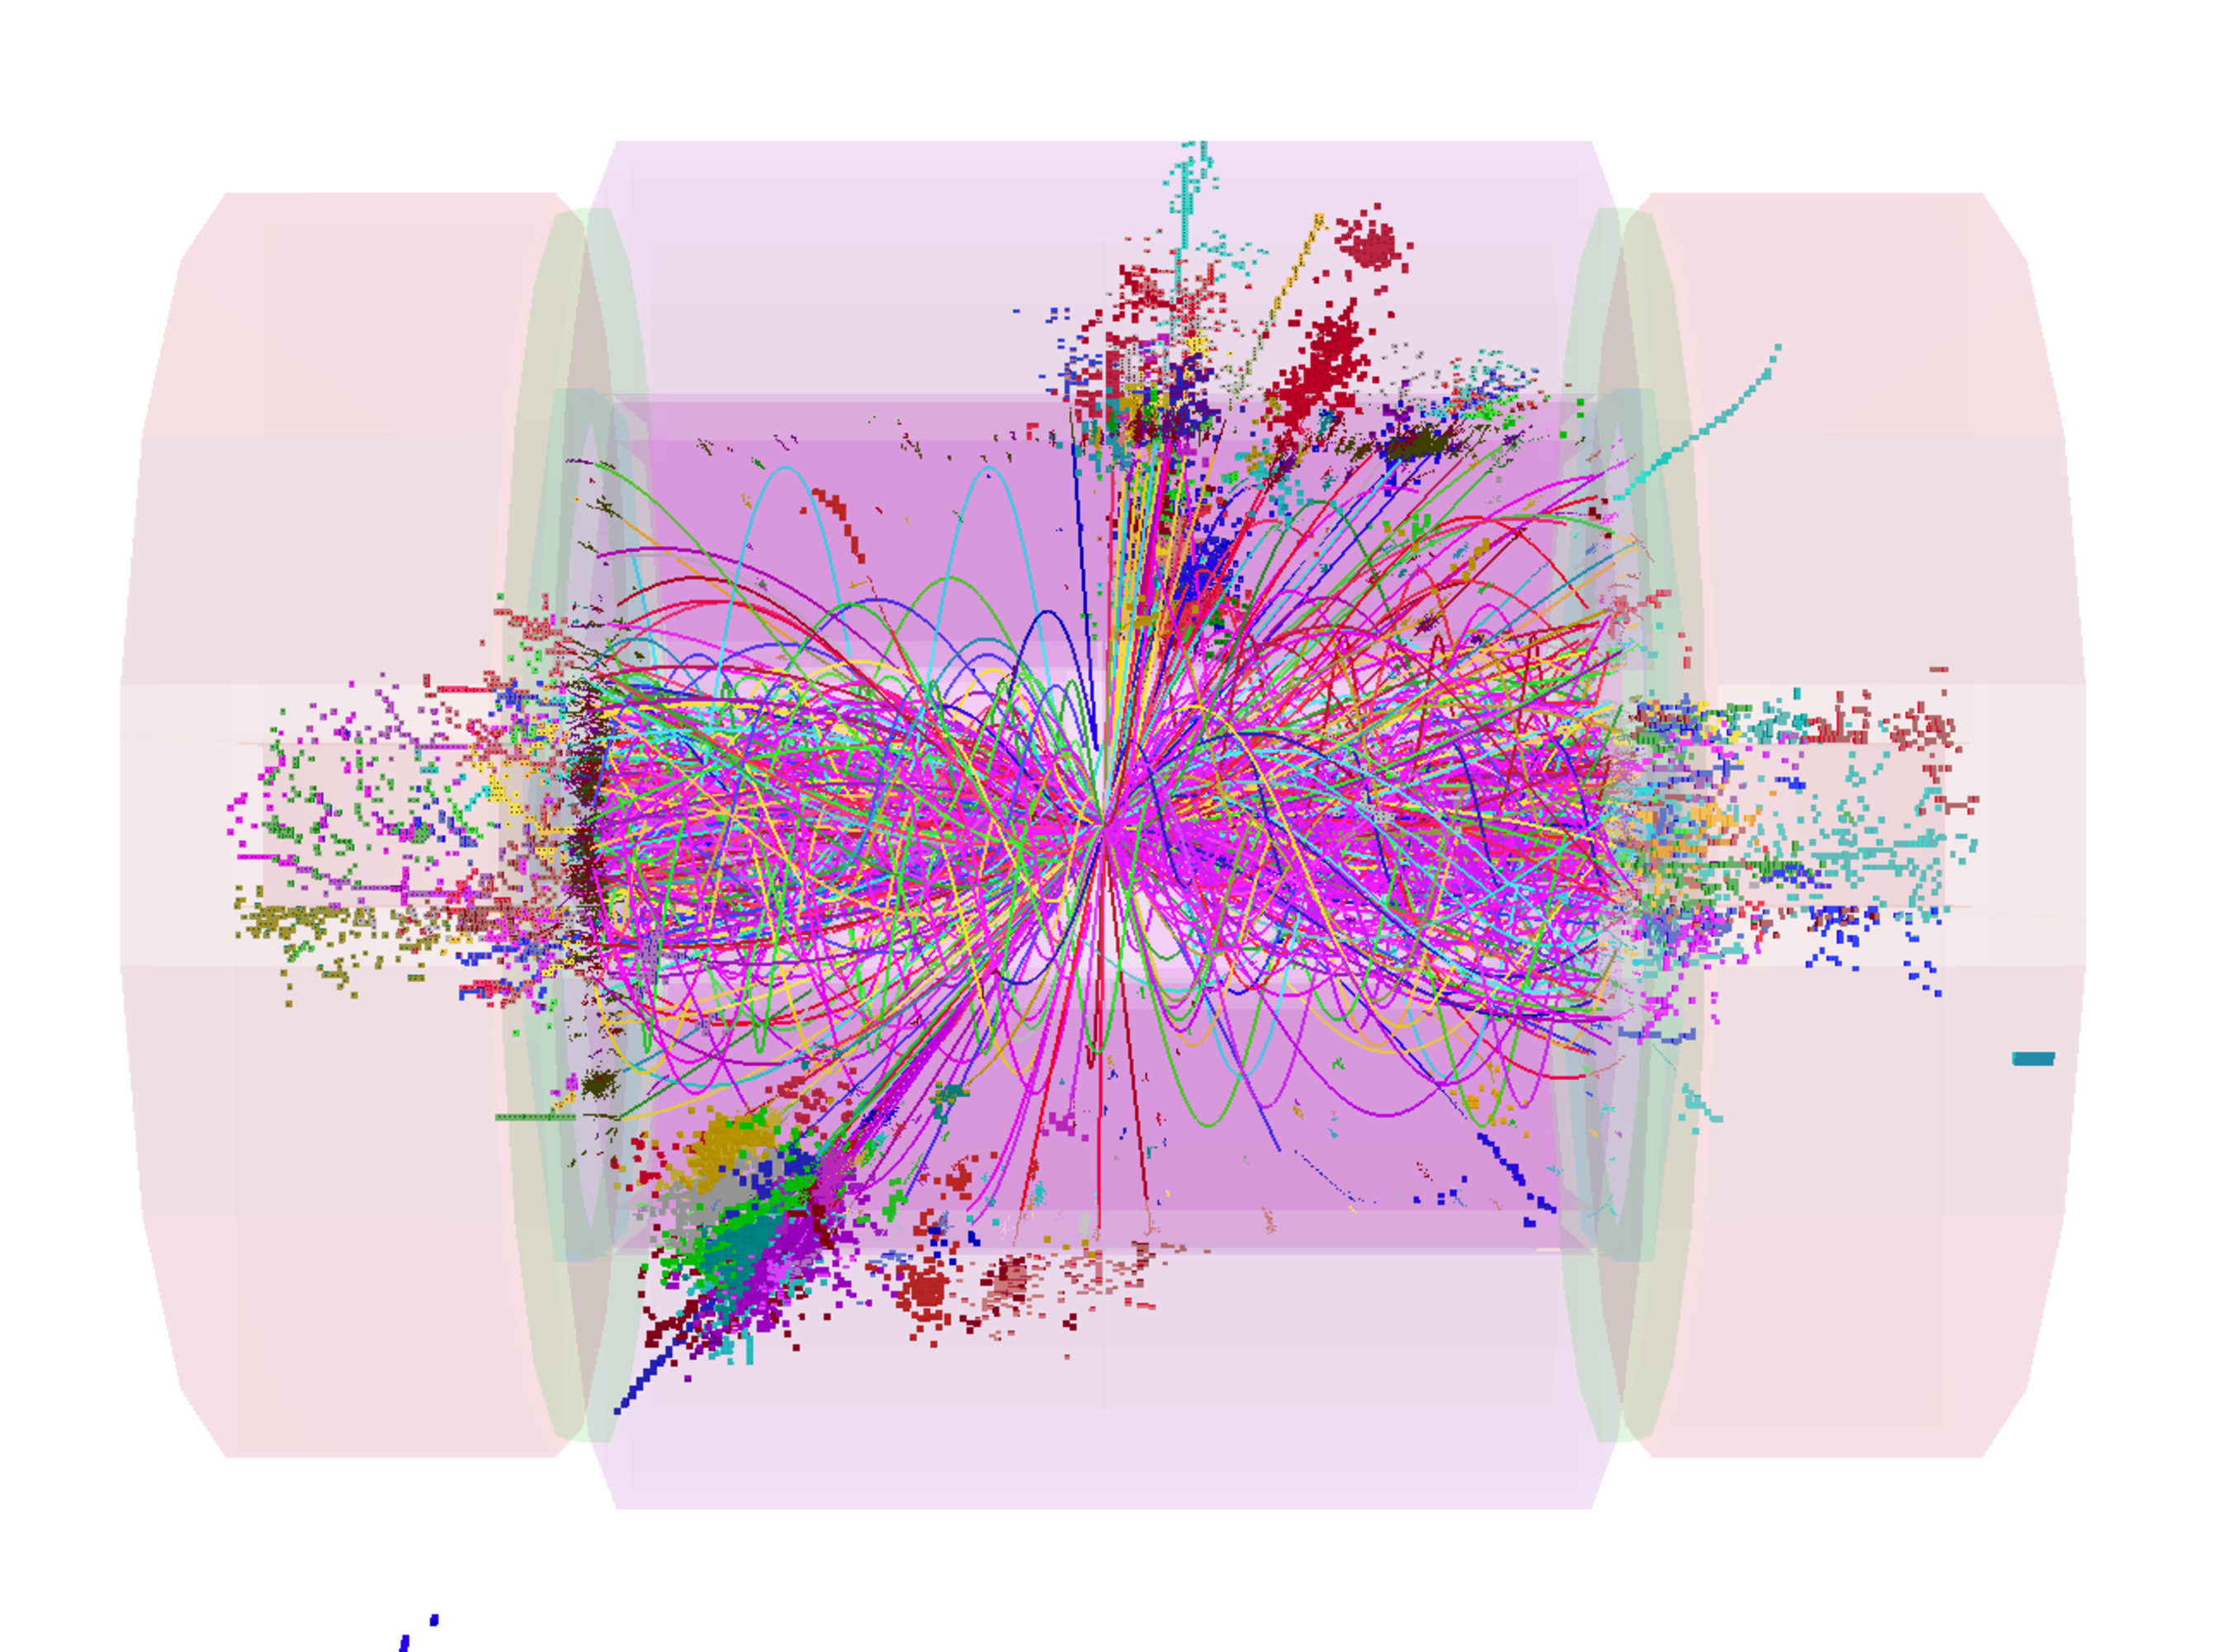
\includegraphics[width=6cm]{HH2.pdf}
\column{6cm}
\centering
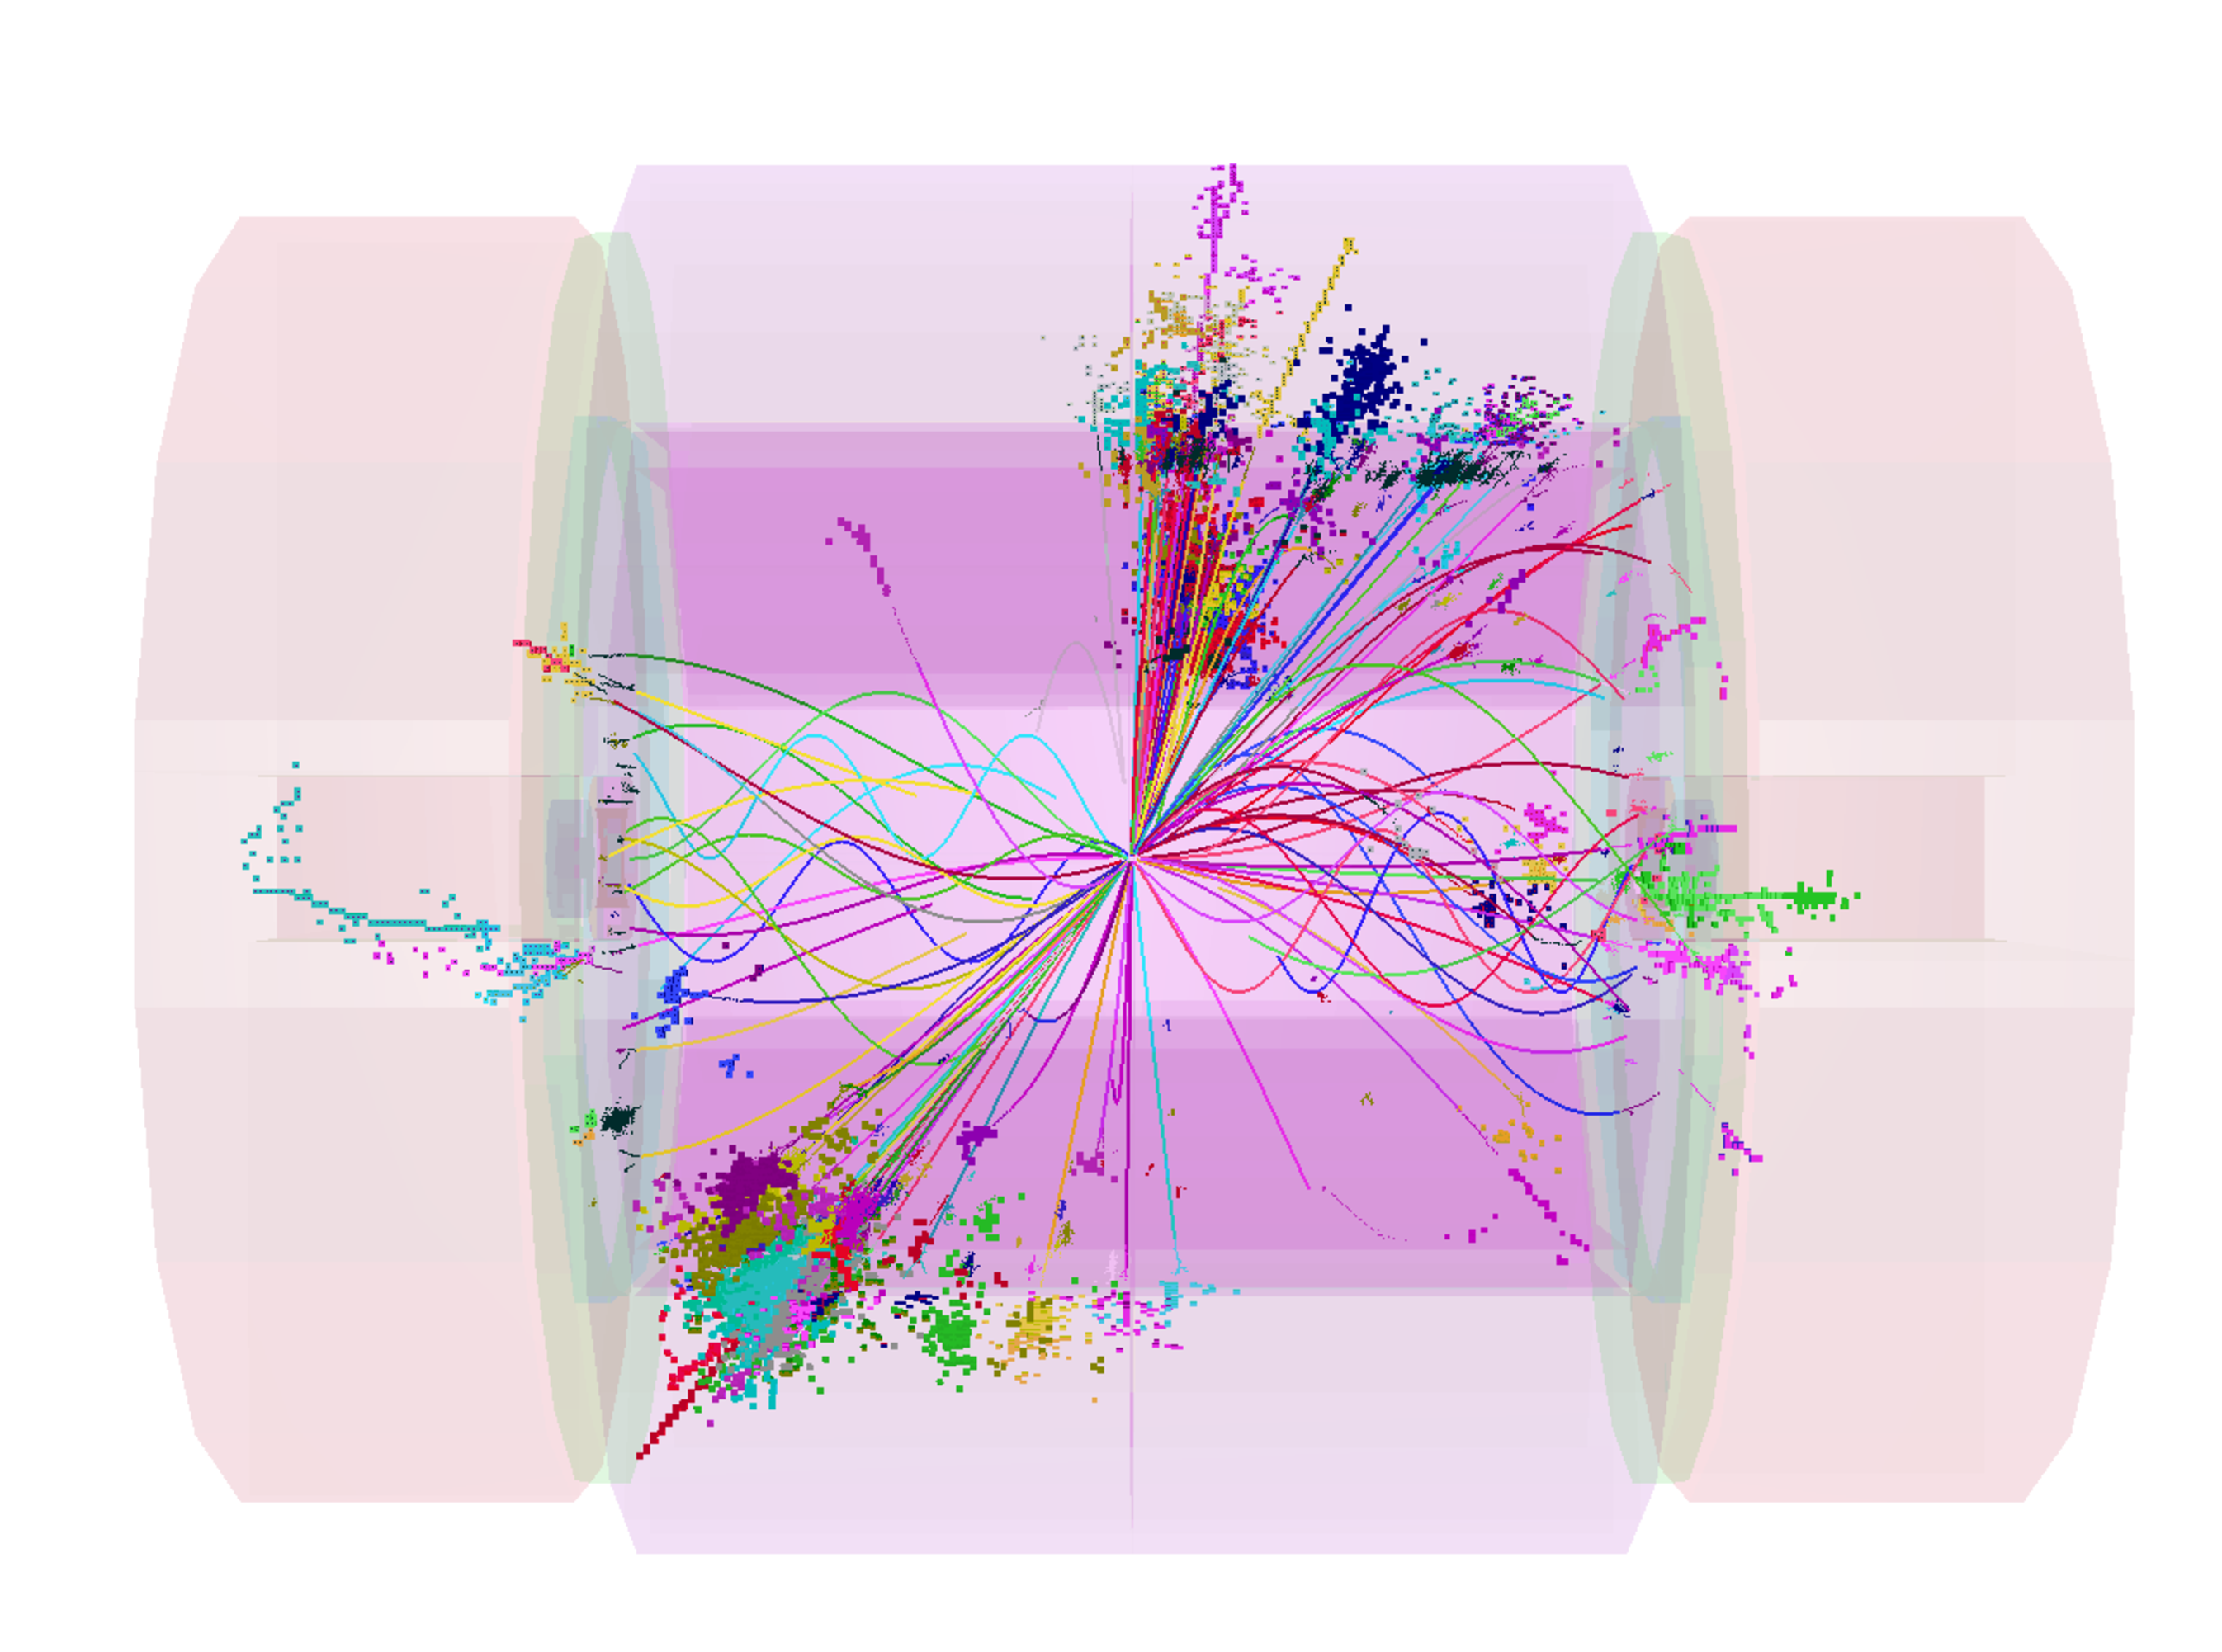
\includegraphics[width=6cm]{HH2tight.pdf}
\end{columns}
\begin{columns}[c]
\column{6cm}
\centering
No cuts:\\ \alert{$\sim1.2\textrm{TeV}$}\\
{\color{blue}{\scriptsize 10ns window}}
\column{6cm}
\centering
Tight timing cuts and jet finding:\\ \alert{$\sim100\textrm{GeV}$}
\end{columns}
~\\
\alert{Using timing cuts and jet finding reduces most of the background}
\end{frame}

\section[Benchmarks]{The benchmark channels}
\begin{frame}
\frametitle{The benchmark channels}
The benchmark channels used to assess detector performance:
\begin{itemize}
\item $\Pep\Pem \to \Ph \Pgne \Pagne, \Ph \to \mu^+\mu^-, \Ph \to
\Pbottom\APbottom$ (SID),
\item  $\Pep\Pem \to \PHp \PHm\to \Ptop\APbottom\APtop\Pbottom$(ILD),\\
$\Pep\Pem \to \PHz \PA\to\Pbottom\APbottom\Pbottom\APbottom$ (ILD),
\item $\Pep\Pem \to \PSq_R \PaSq_R\to\Pquark\APquark\PSgxz_1\PSgxz_1$ (ILD), 
\item $\Pep\Pem \to \PSl \PaSl \,(\ell = \Pe,\Pgm,\Pgne)$ (ILD), 
\item $\Pep\Pem \to \PSgxpm_1 \PSgxmp_1\to\PWp\PWm\PSgxz_1\PSgxz_1$ (SID),\\
$\Pep\Pem \to \PSgxz_2 \PSgxz_2\to \Ph\Ph\PSgxz_1\PSgxz_1$ (SID),
\item  $\Pep\Pem \to \Pqt \Paqt$ (500~GeV, ILD).
\end{itemize}
\end{frame}
\begin{frame}
\frametitle{SM Higgs decays}
Flavour tagging ($\Ph\to\Pbottom\APbottom$):
\begin{columns}[c]
\column{4cm}
\centering
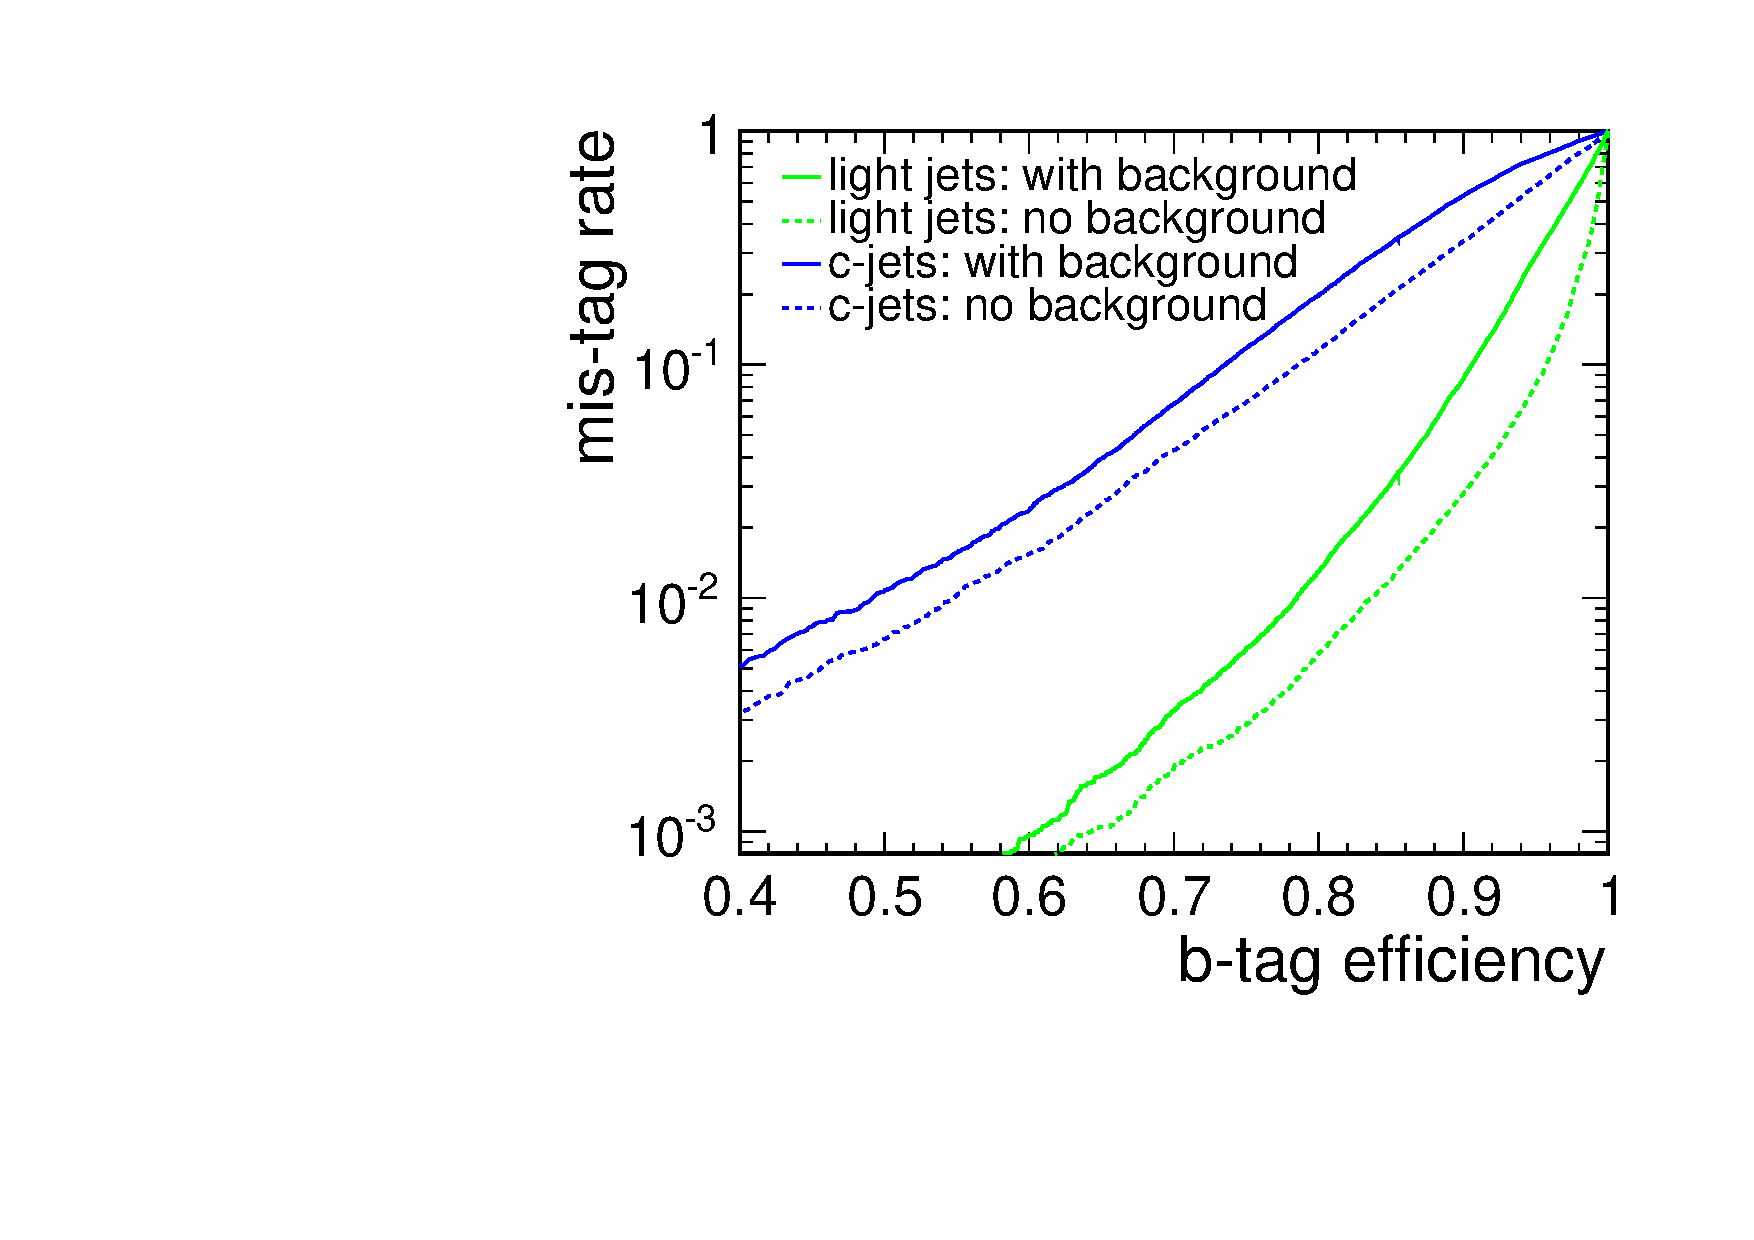
\includegraphics[width=4cm]{Light_Higgs_Flavour_Tag.pdf}
\column{4cm}
\centering
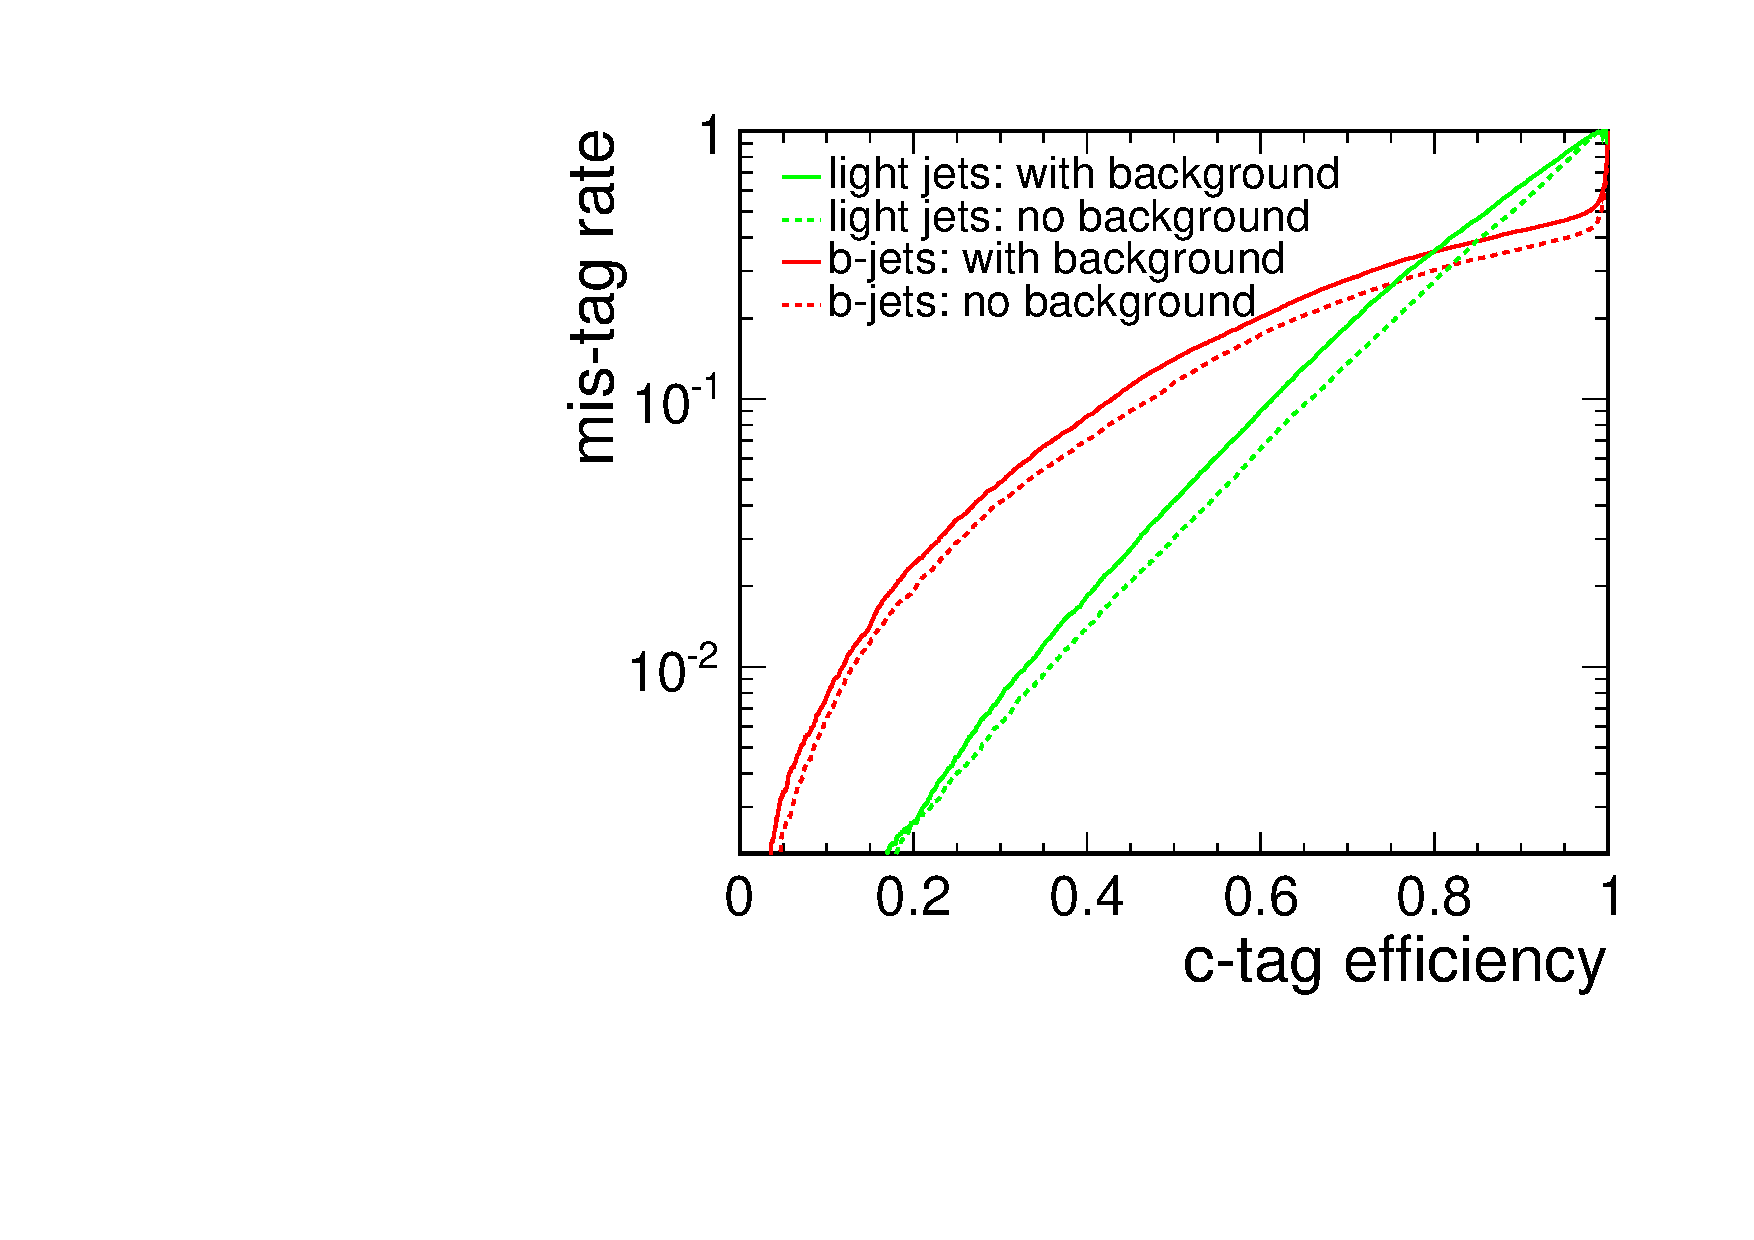
\includegraphics[width=4cm]{Light_Higgs_Flavour_Tag_C.pdf}
\end{columns}
Tracking efficiency ($\Ph\to\mu\mu$):
\begin{columns}[c]
\column{4cm}
\centering
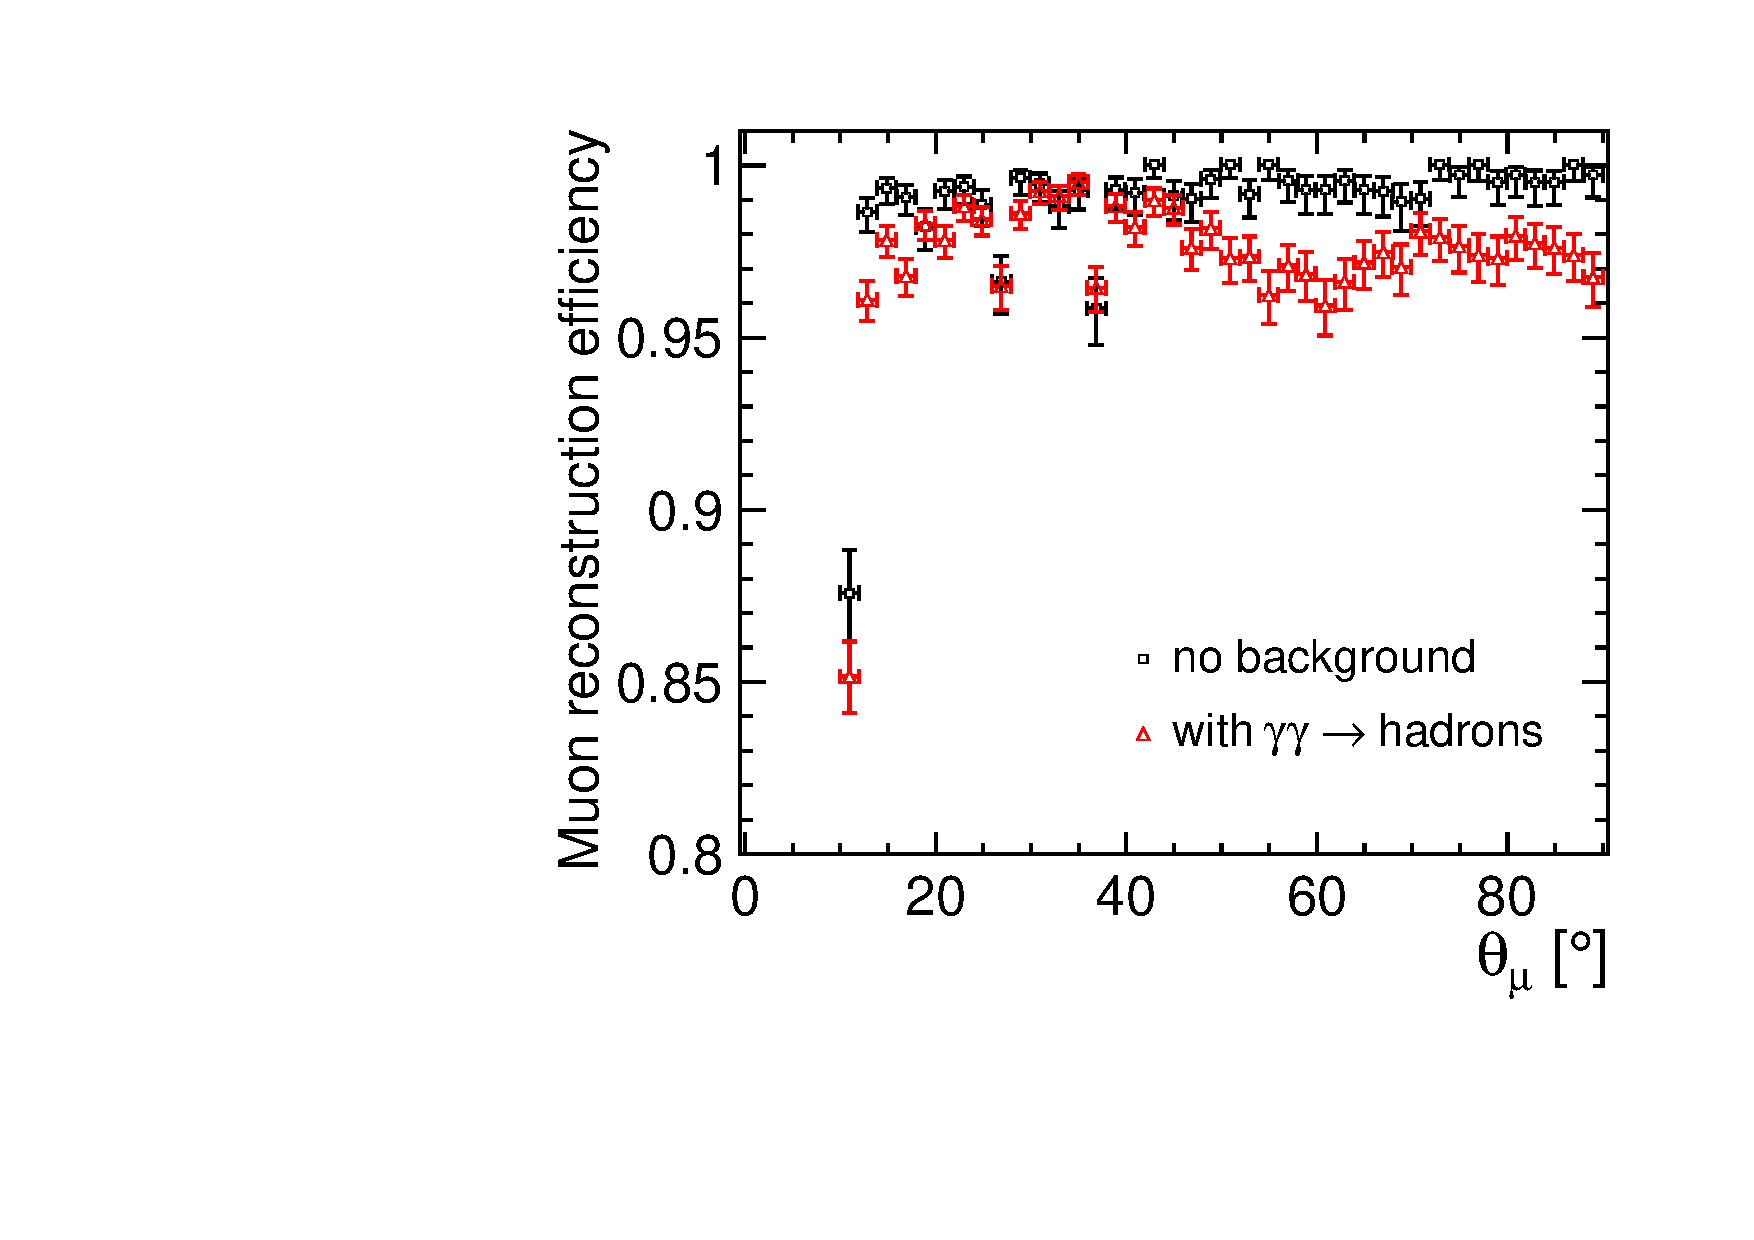
\includegraphics[width=4cm]{MuonEfficiency2.pdf}
\column{4cm}
\centering
%\includegraphics[width=4cm]{}
\end{columns}
\end{frame}

\begin{frame}
\frametitle{SM Higgs decays}
\begin{columns}[c]
\column{6cm}
\centering
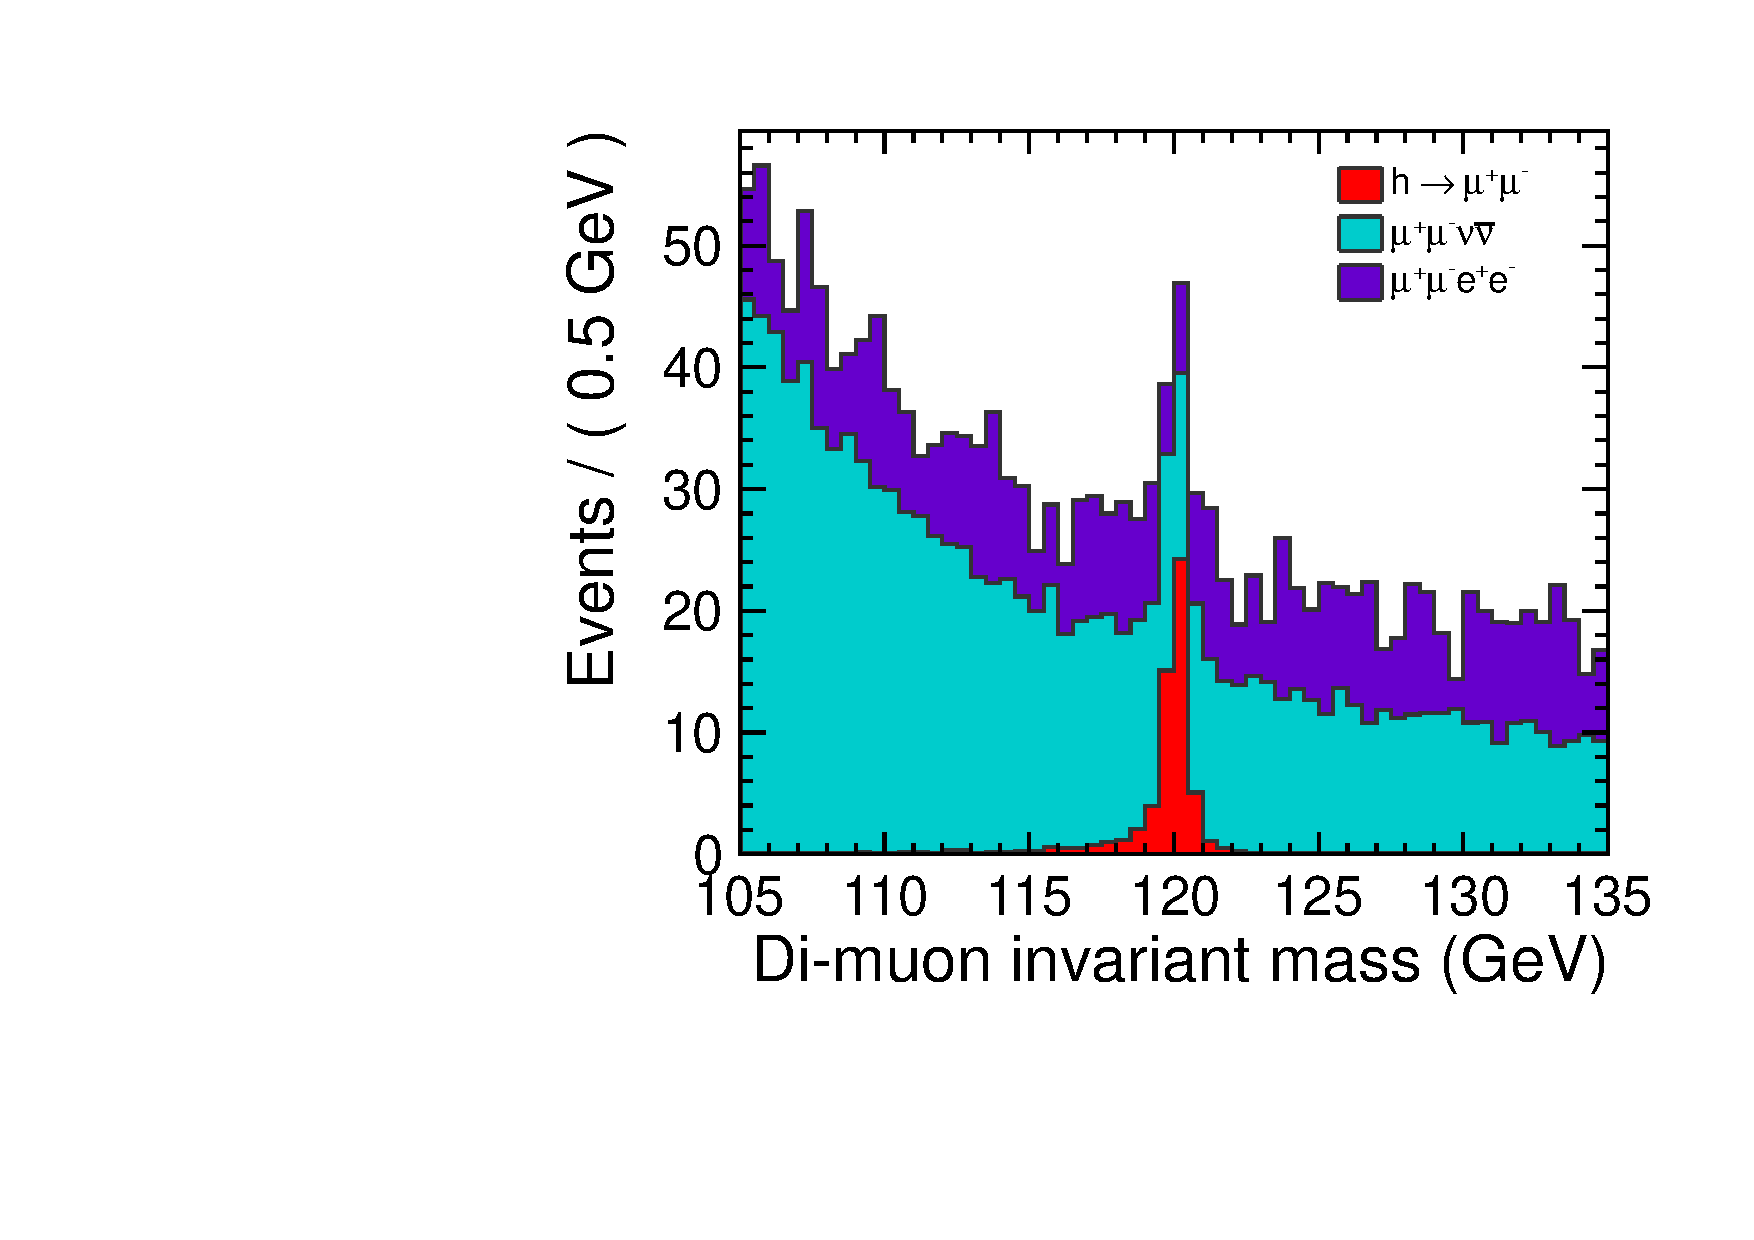
\includegraphics[width=5cm]{ee_h_mumu_mass_mh120GeV}
\column{6cm}
\centering
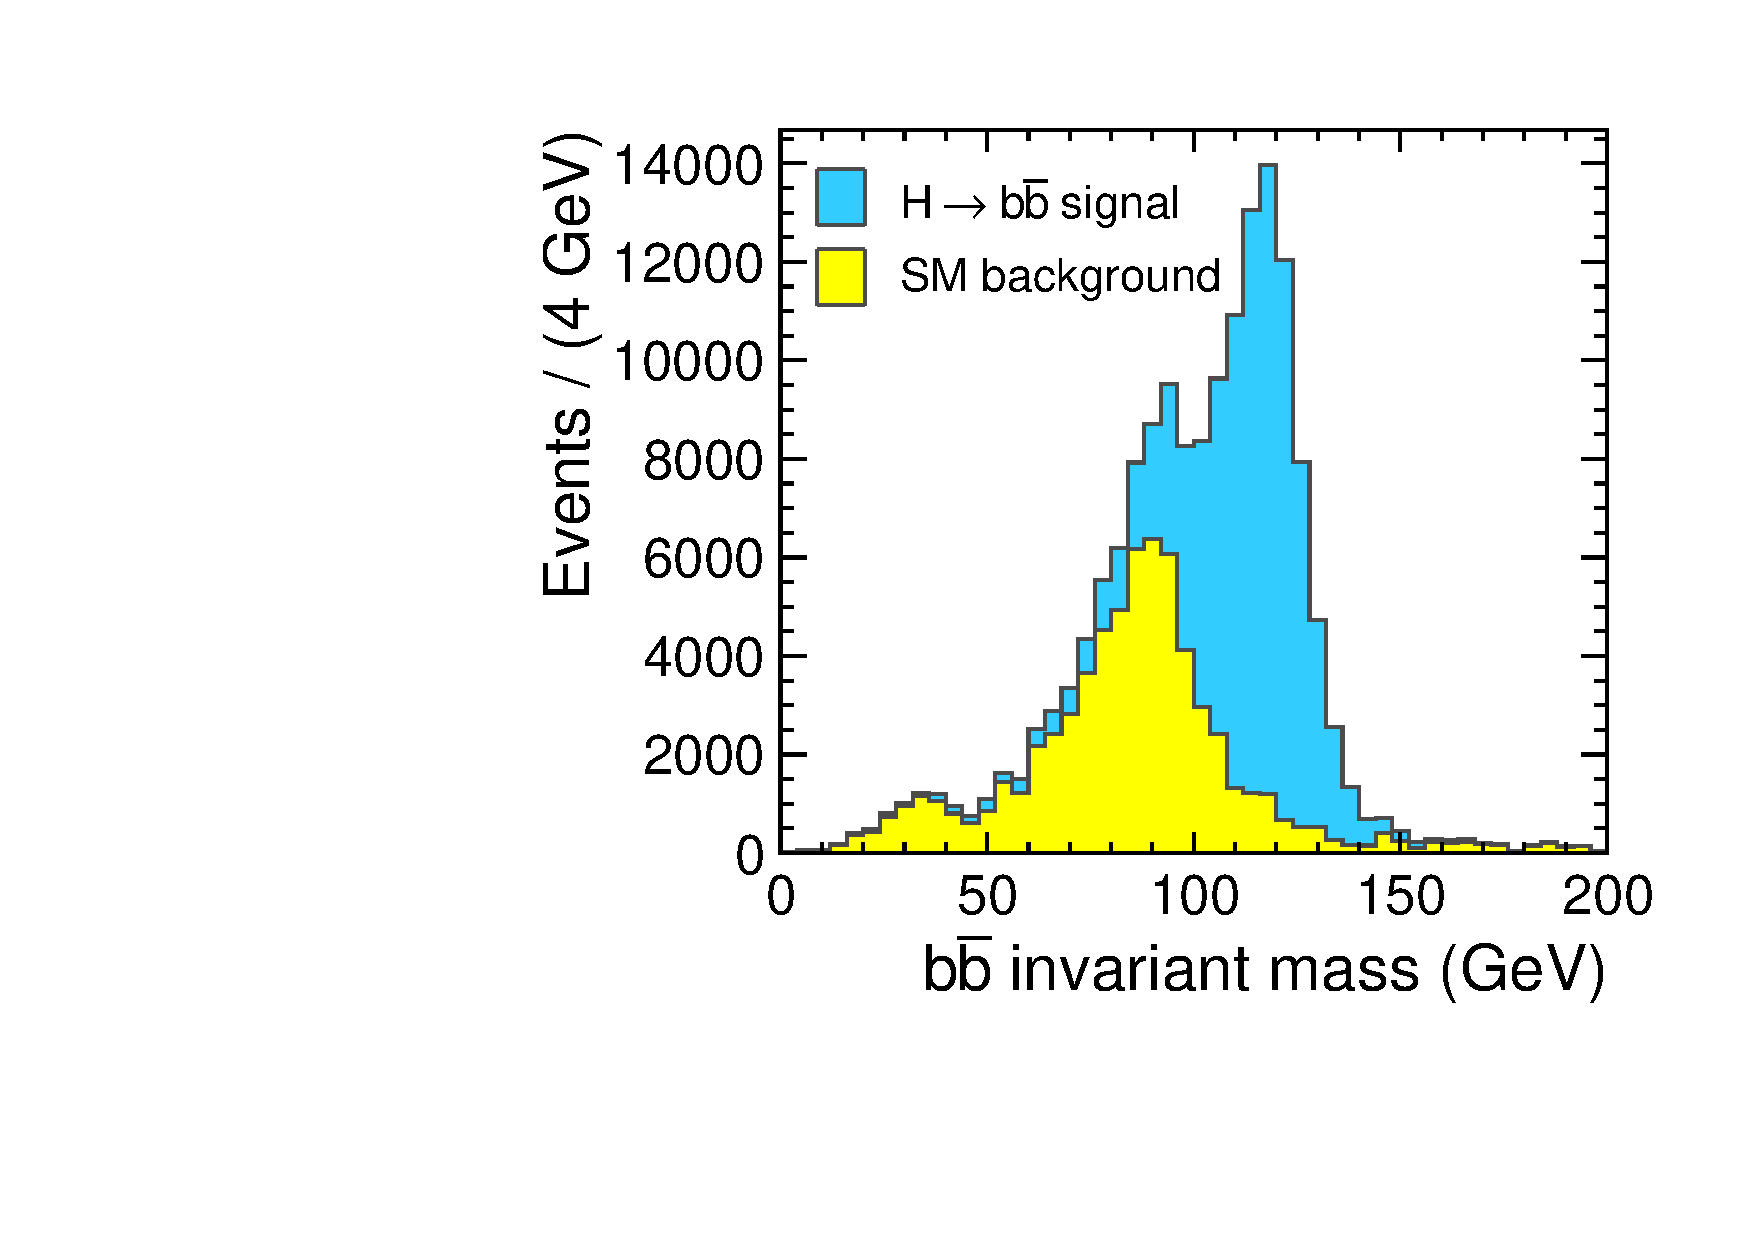
\includegraphics[width=5cm]{ee_h_bb_mass_mh120GeV}
\end{columns}
Cross section measurements:
\begin{itemize}
  \item
  $\sigma(\sigma_{\Ph\to\Pbottom\APbottom})/\sigma_{\Ph\to\Pbottom\APbottom} =
  0.22\%$ stat.
  \item $\sigma(\sigma_{\Ph\to\Pmuon\APmuon})/\sigma_{\Ph\to\Pmuon\APmuon}
  = 15.7\%$ stat.
\end{itemize}
\end{frame}


\begin{frame}
\frametitle{Gauginos}
{\footnotesize $\Pep\Pem \to \PSgxpm_1 \PSgxmp_1\to\PWp\PWm\PSgxz_1\PSgxz_1$ and
$\Pep\Pem \to \PSgxz_2 \PSgxz_2\to \Ph\Ph\PSgxz_1\PSgxz_1$}
\begin{columns}[c]
\column{6cm}
\centering
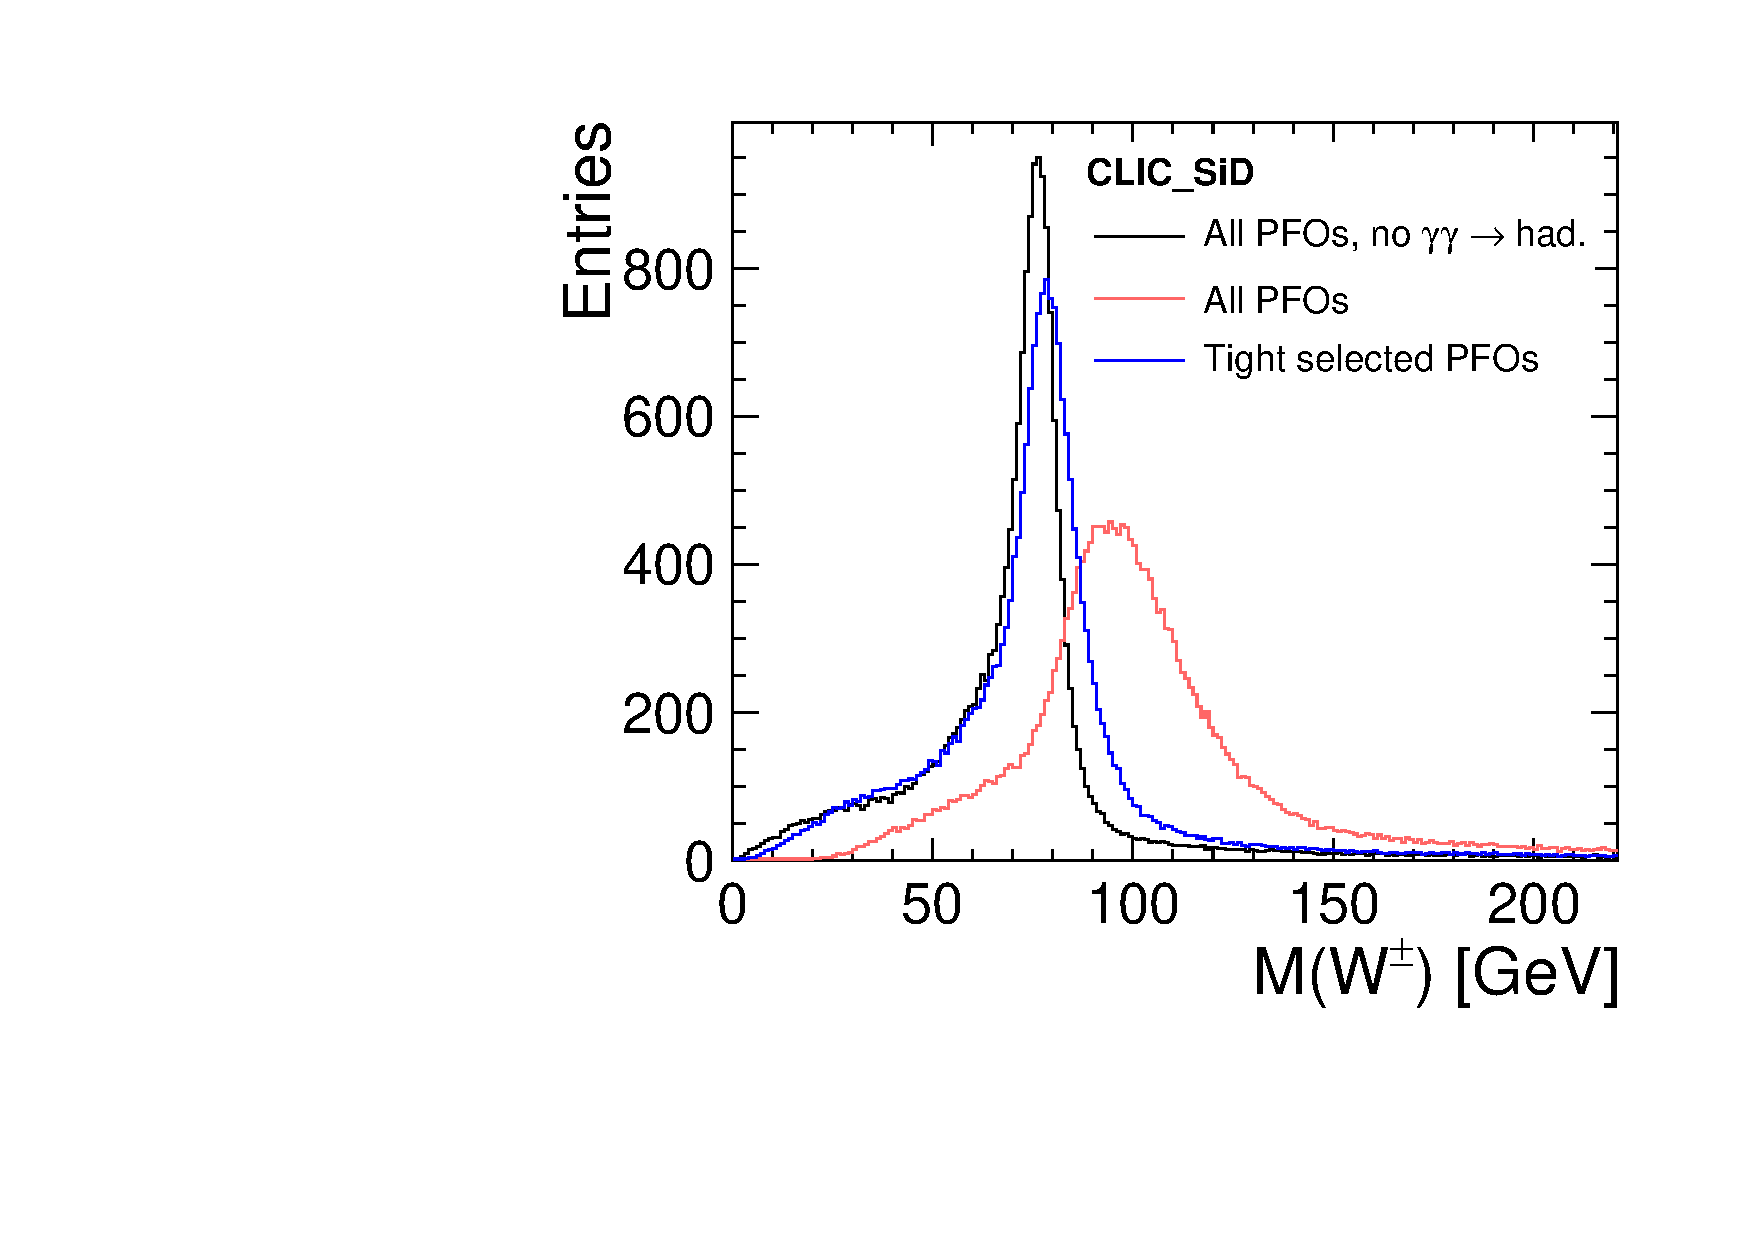
\includegraphics[width=6cm]{W_reconstruction_mass.pdf}
\column{6cm}
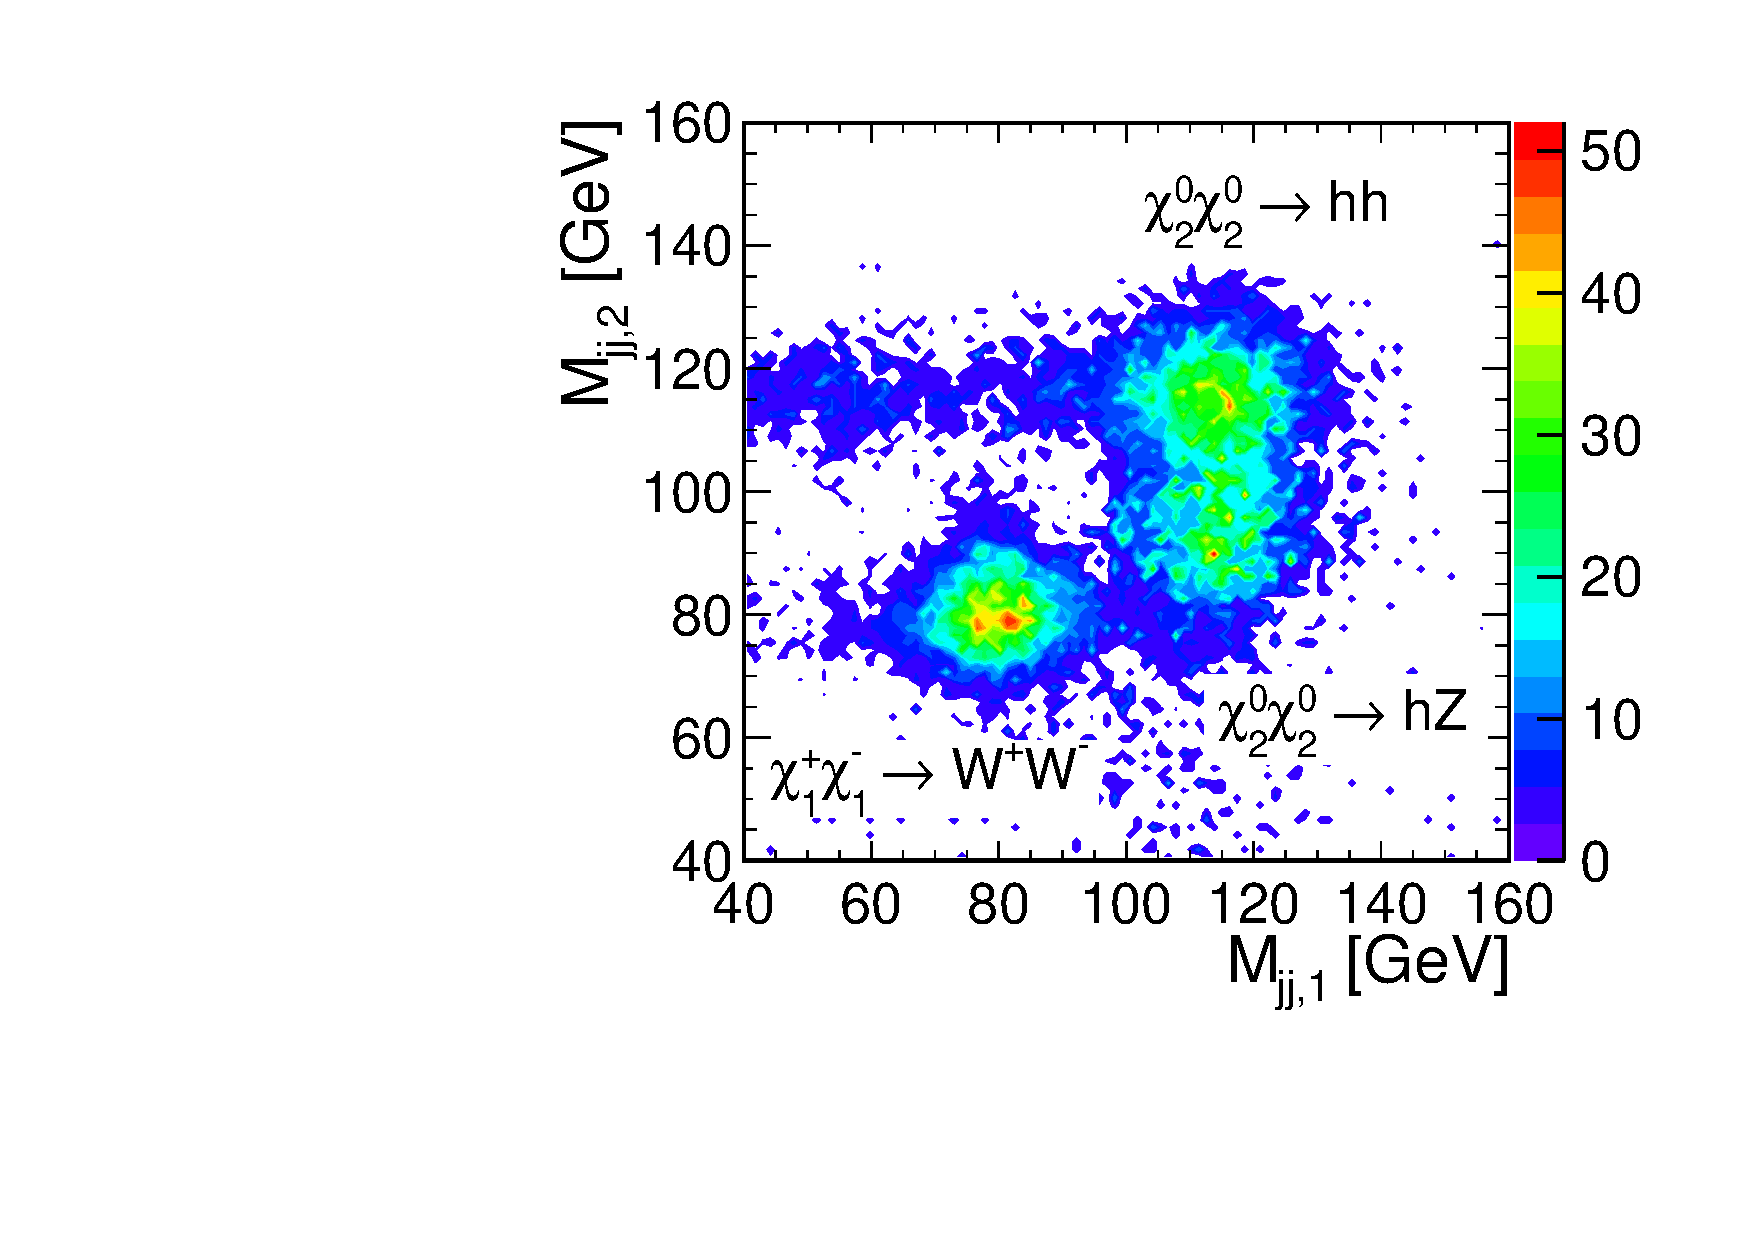
\includegraphics[width=6cm]{../WhizardWorkshop/MassPlot2D}
\end{columns}
\alert{Test of jet energy resolution}
\end{frame}
\begin{frame}
\frametitle{Gauginos}
\begin{columns}[c]
\column{4.5cm}
\centering
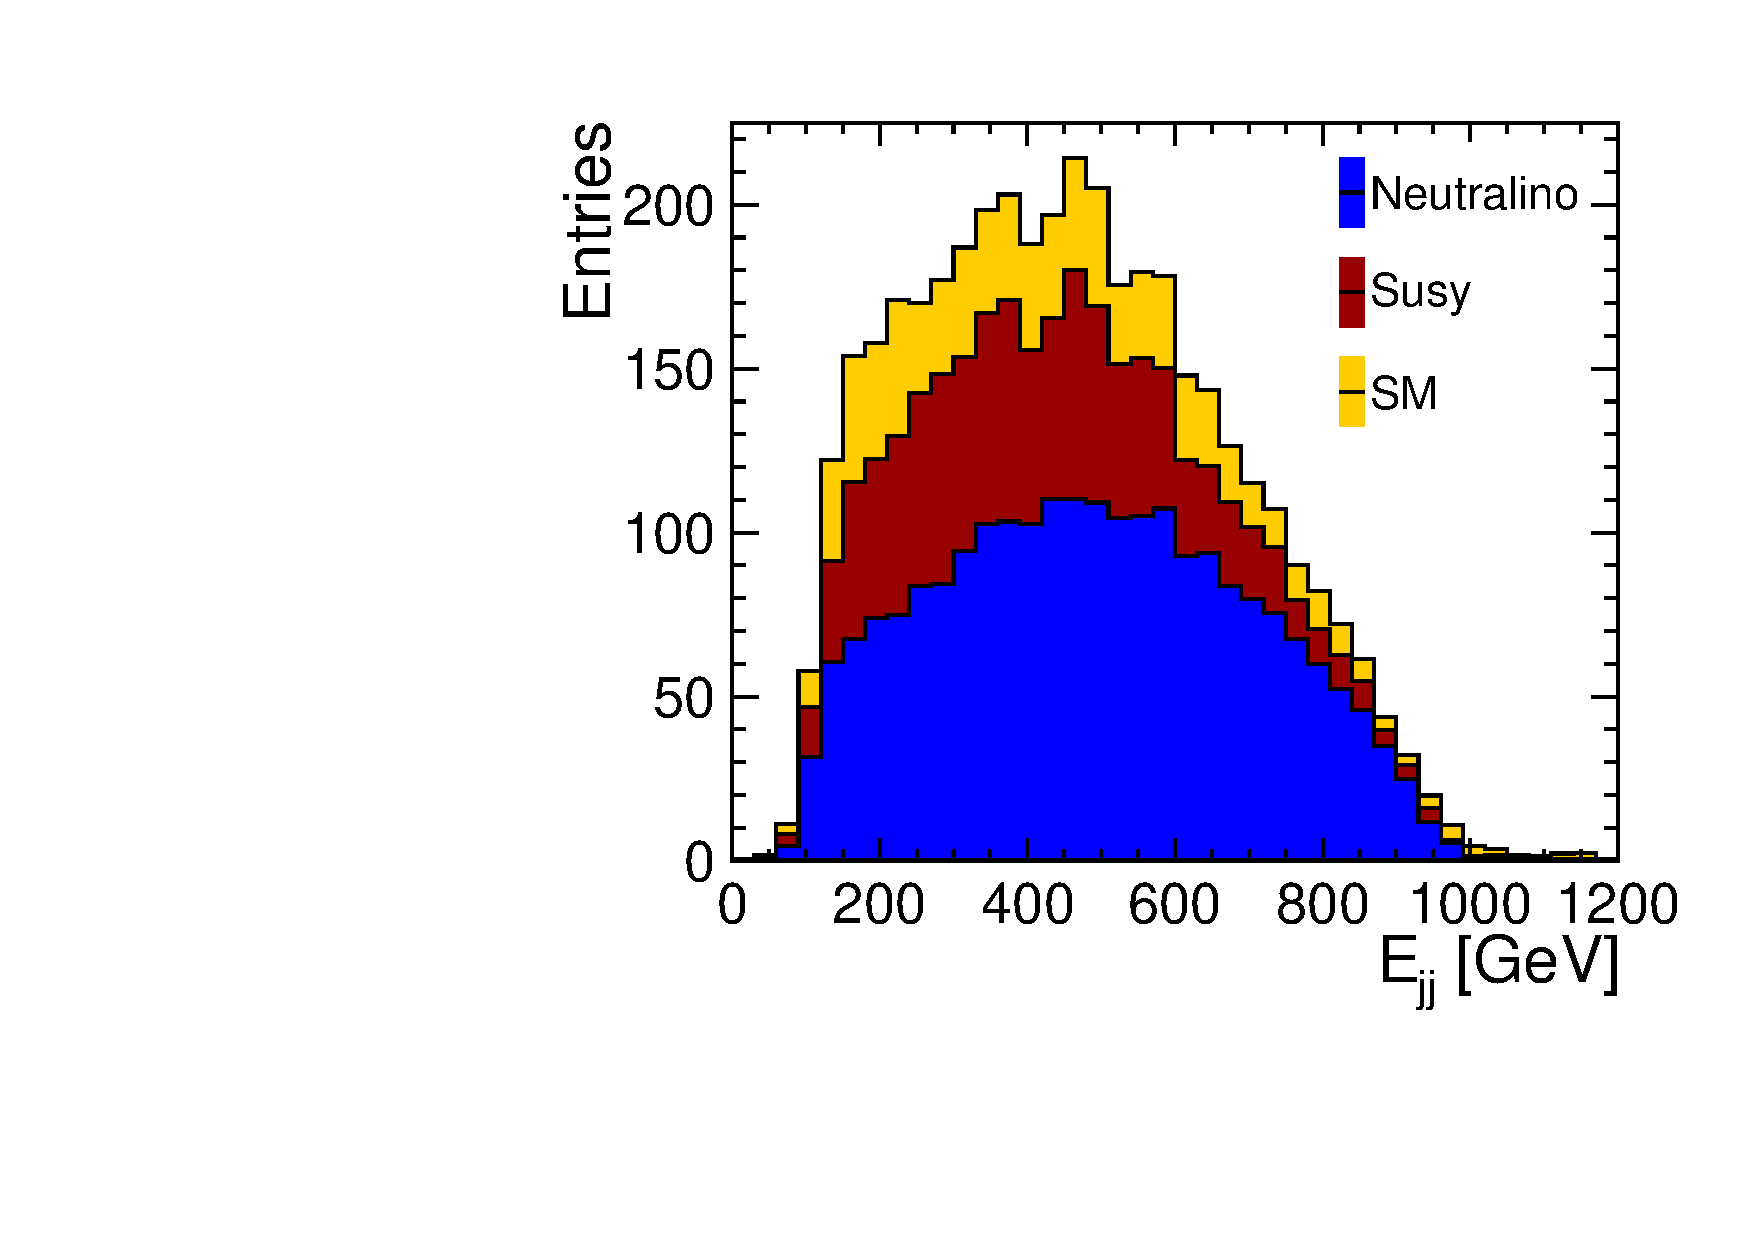
\includegraphics[width=4.5cm]{NeutralinoSel_E.pdf}\\
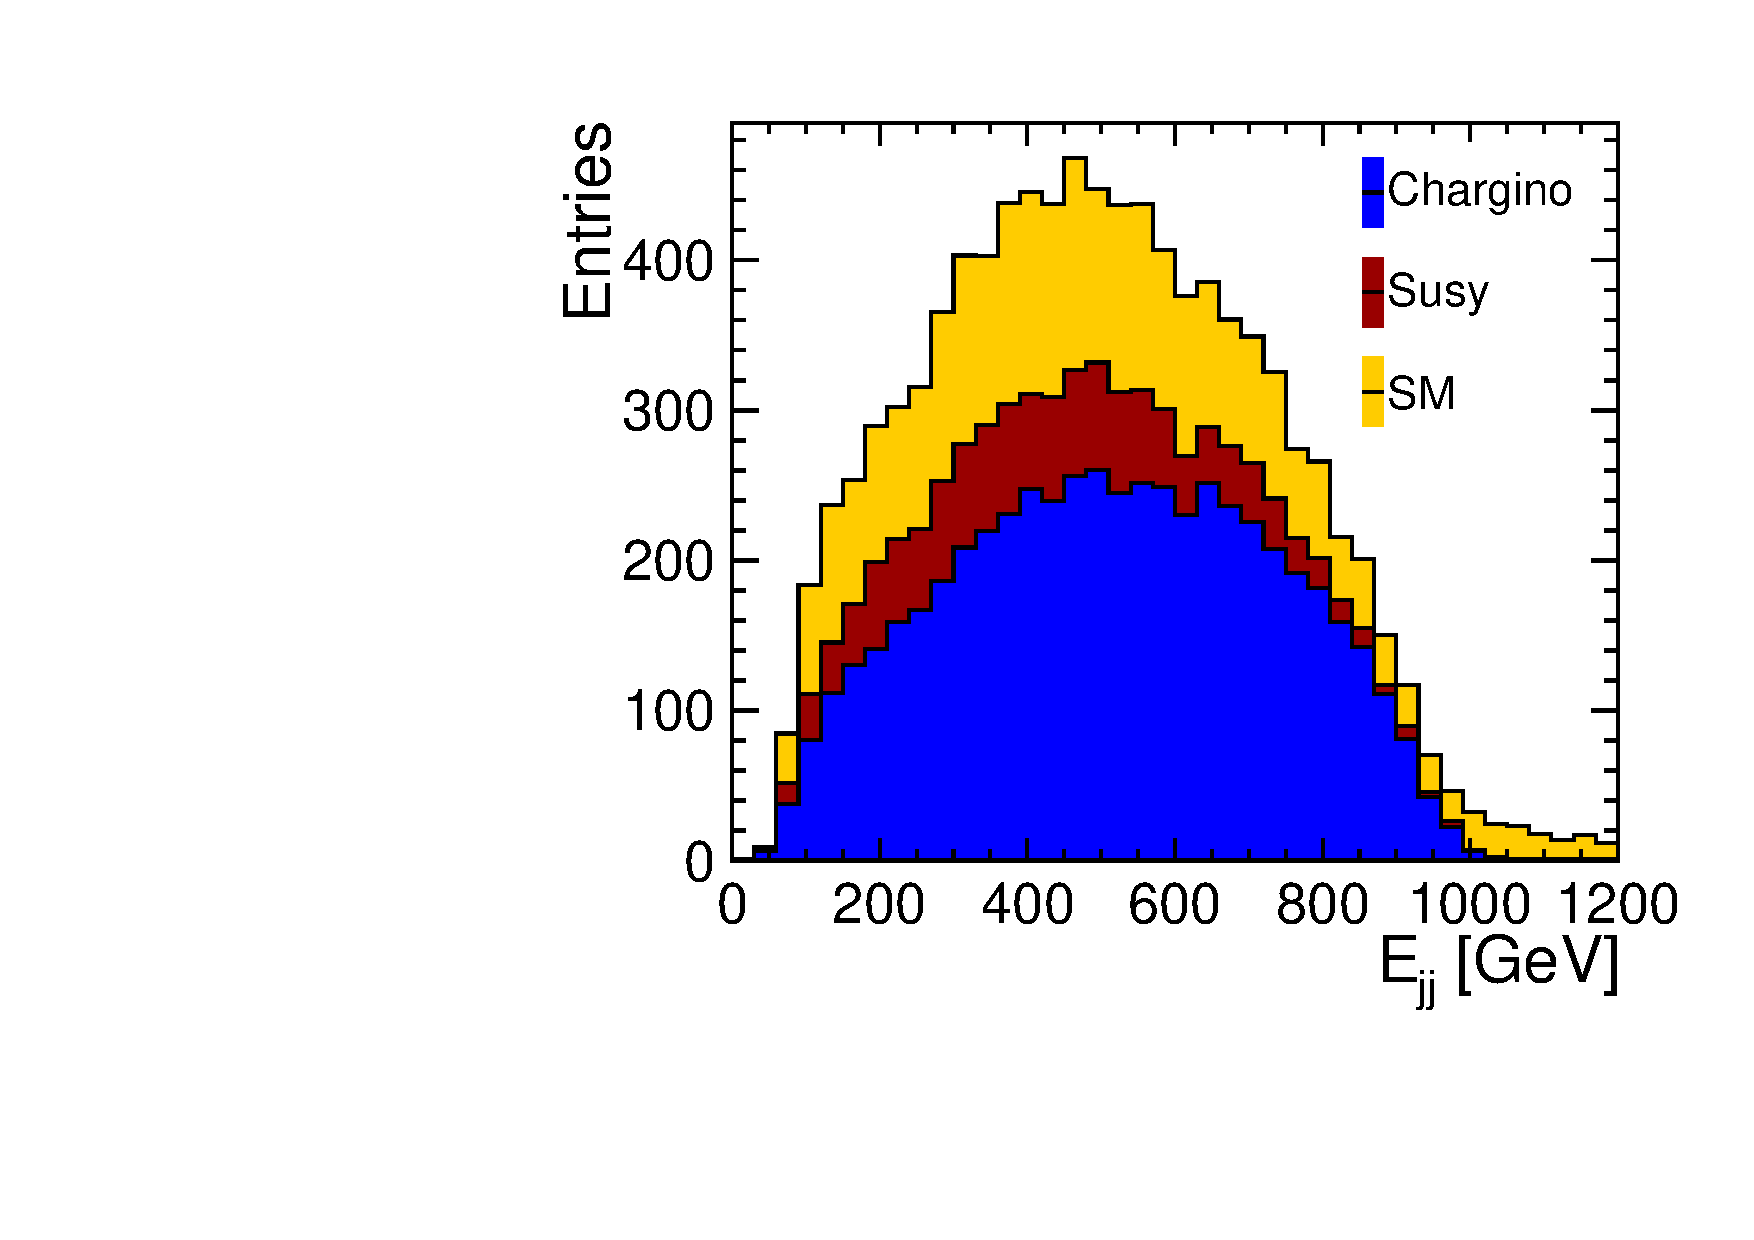
\includegraphics[width=4.5cm]{CharginoSel_E.pdf}
\column{4.5cm}
\centering
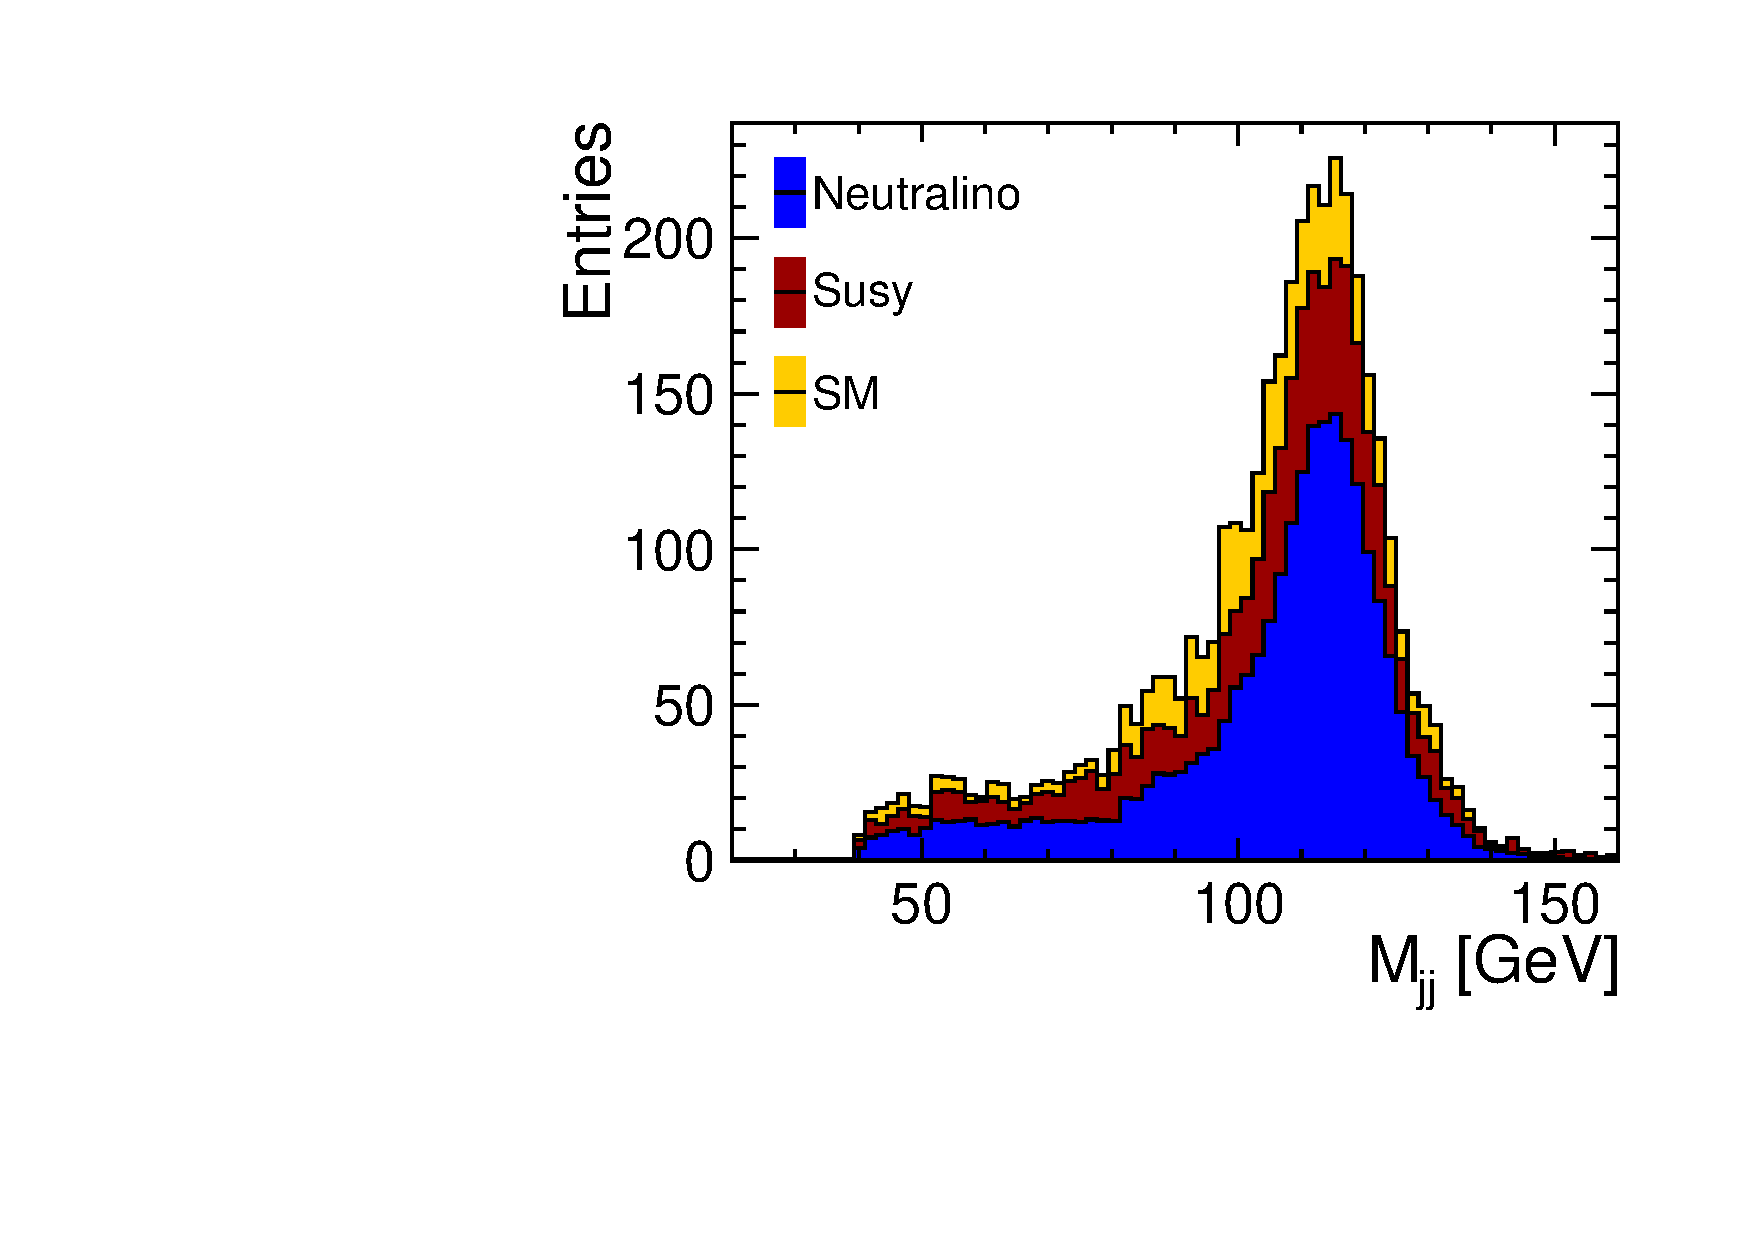
\includegraphics[width=4.5cm]{NeutralinoSel_M.pdf}\\
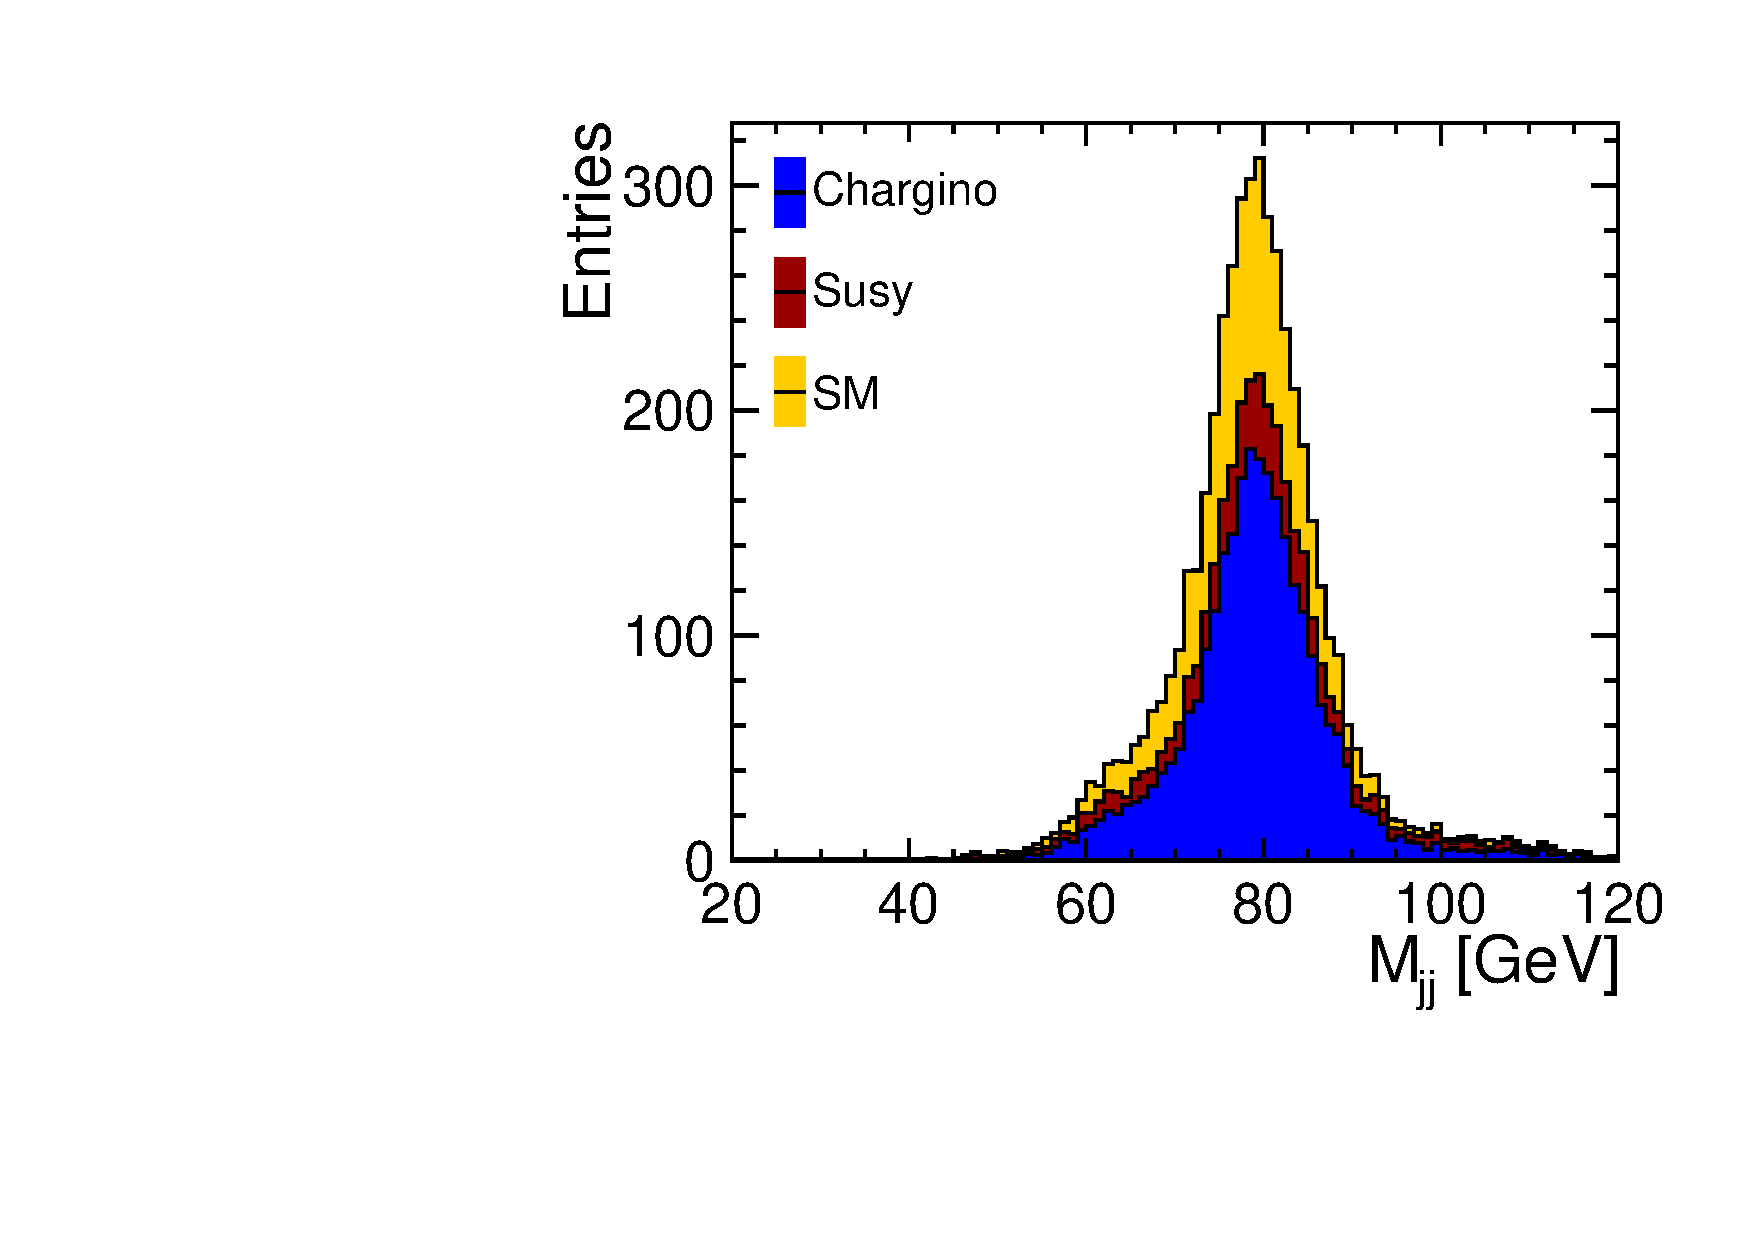
\includegraphics[width=4.5cm]{CharginoSel_M.pdf}
\end{columns}
\end{frame}
\begin{frame}
\frametitle{Gauginos}
\begin{center}
\begin{tabular}{c c c c}
       \toprule
       Parameter 1                & Uncertainty &          Parameter 2 & Uncertainty \\
       \midrule
       $M(\tilde{\chi}_{1}^{\pm})$ & $6.3$~GeV & $\sigma(\tilde{\chi}_{1}^{+}\tilde{\chi}_{1}^{-})$  & $2.2$\% \\
       $M(\tilde{\chi}_{1}^{0})$   & $3.0$~GeV & $\sigma(\tilde{\chi}_{1}^{+}\tilde{\chi}_{1}^{-})$  & $1.8$\% \\
       $M(\tilde{\chi}_{2}^{0})$   & $7.3$~GeV & $\sigma(\tilde{\chi}_{2}^{0}\tilde{\chi}_{2}^{0})$  & $2.9$\% \\
\end{tabular}
\end{center}
\end{frame}


\section{Summary}
\begin{frame}
\frametitle{Conclusions}
Document printed in Feb 2012, executive summary later in the year
\begin{itemize}
  \item CDR is here:  \url{https://edms.cern.ch/document/1160419}
  \item Sign the CDR here:
  \url{https://indico.cern.ch/conferenceDisplay.py?confId=136364}
\end{itemize}
\end{frame}

\appendix


\begin{frame}
\frametitle{Heavy Higgs: $\PH^0\PA\to\Pbottom\APbottom\Pbottom\APbottom$,
$\PH^+\PH^-\to\Ptop\APbottom\Pbottom\APtop$}
\centering
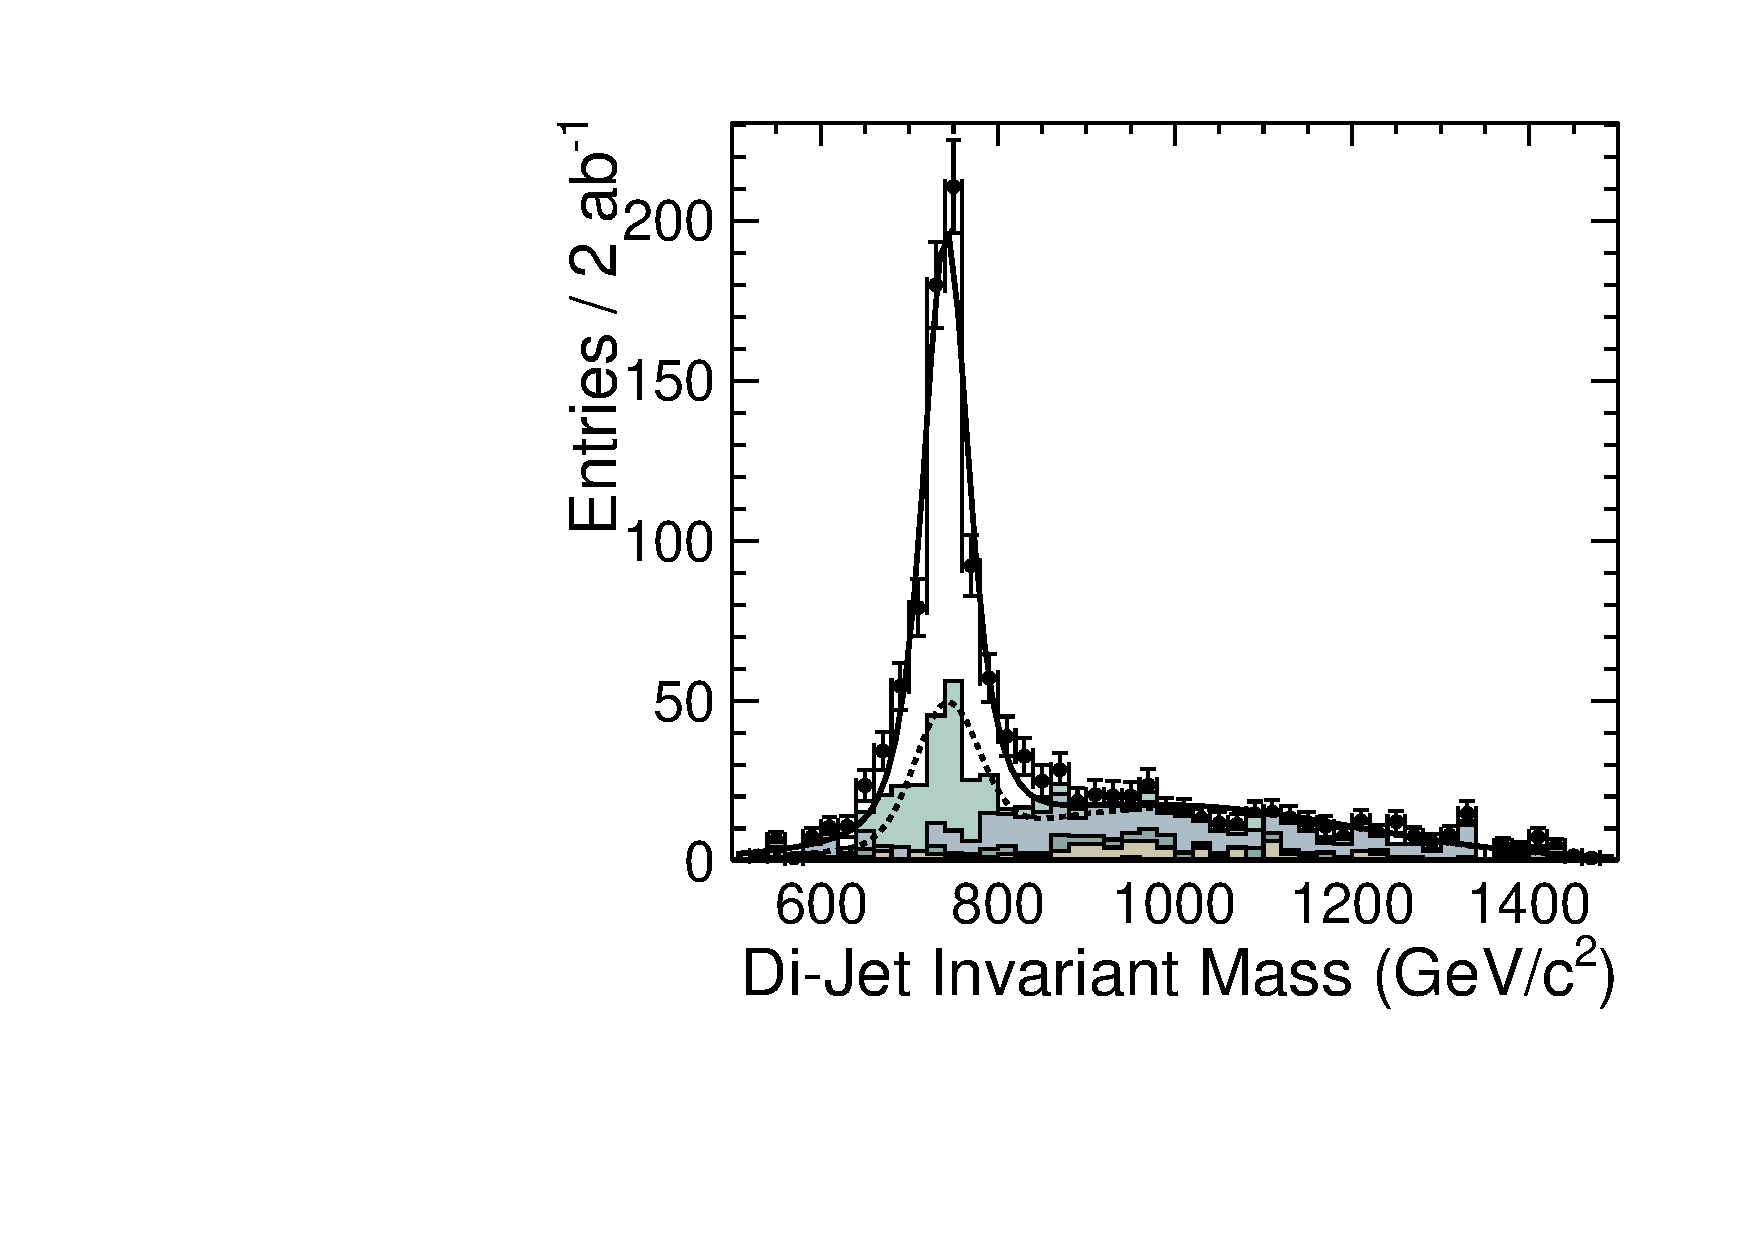
\includegraphics[width=4cm]{HAMass742_Bkg_CKFM_00BX_FJ.pdf}
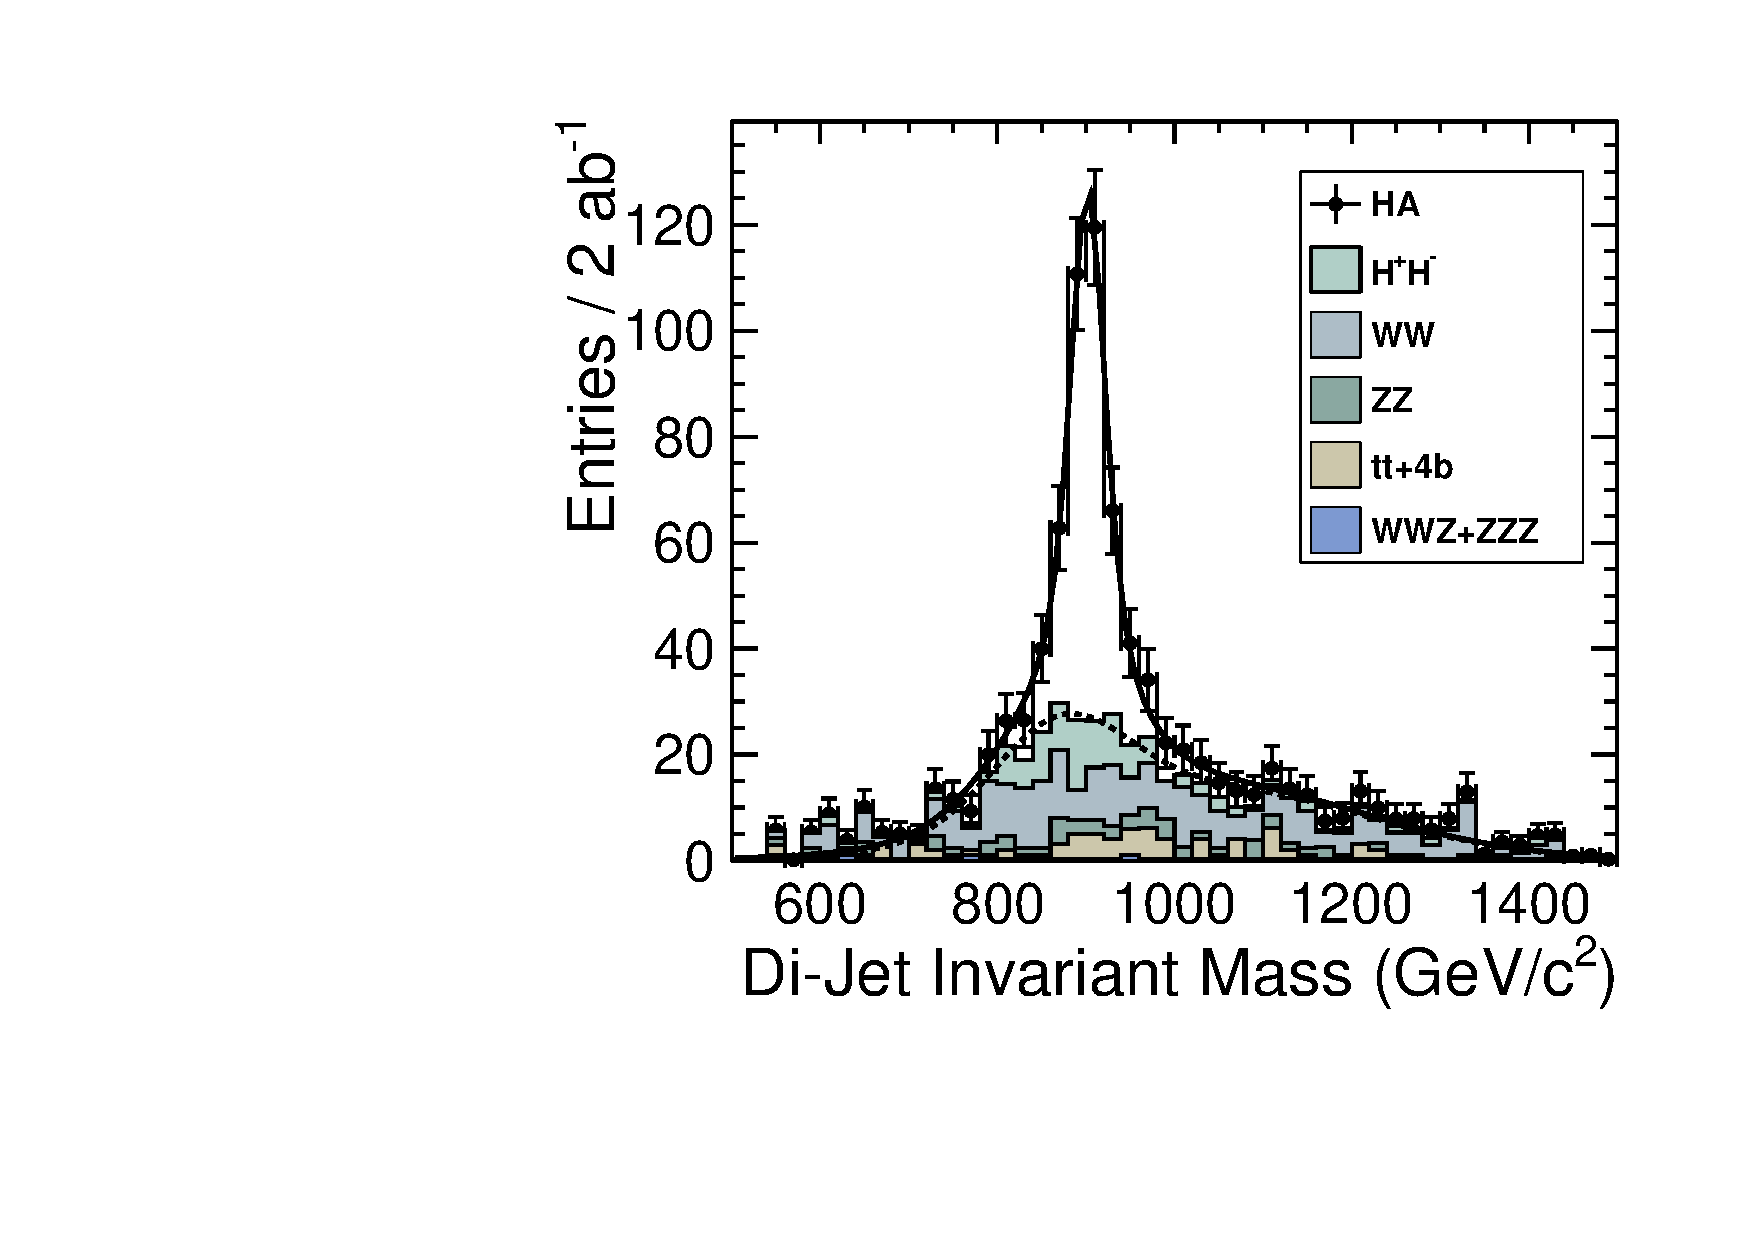
\includegraphics[width=4cm]{HAMass902_Bkg_CKFM_00BX_FJ.pdf}\\
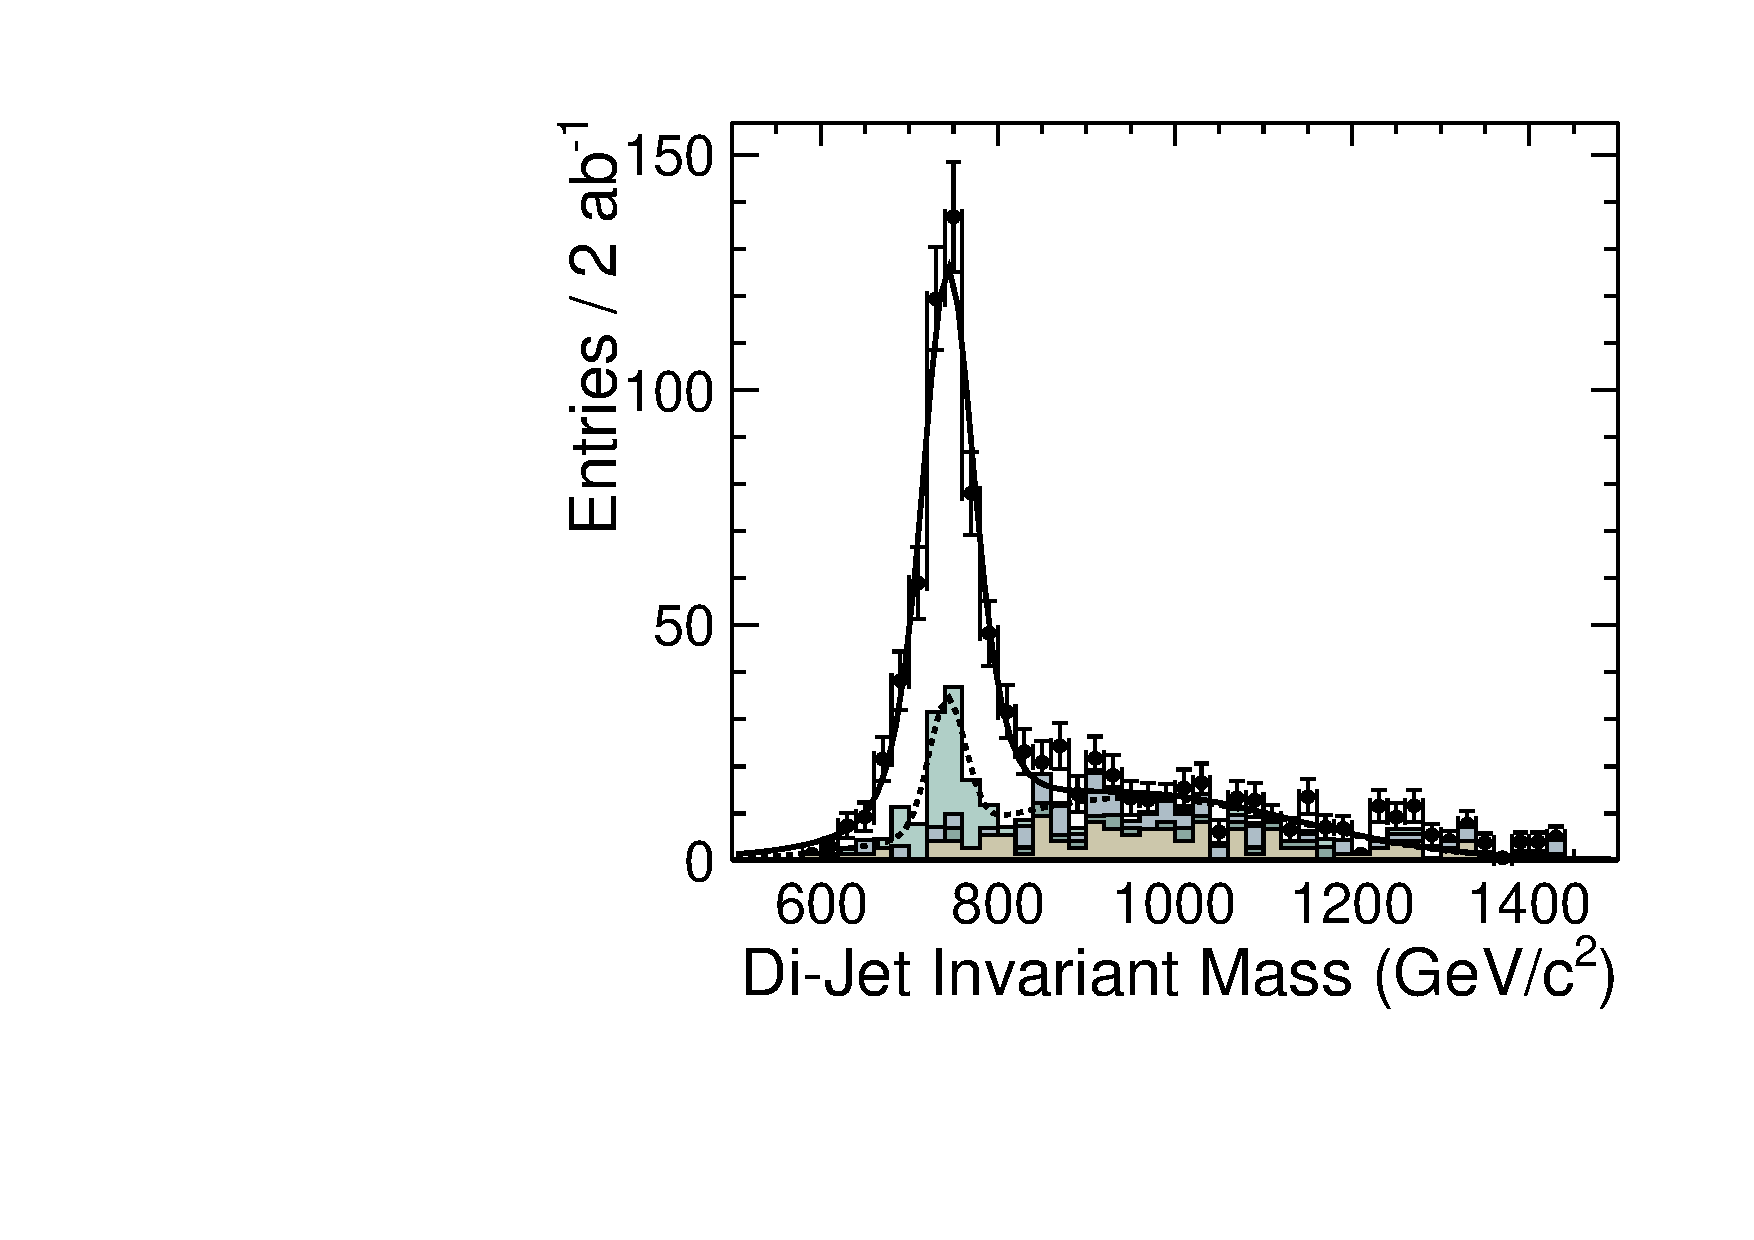
\includegraphics[width=4cm]{Hpm_Mass742_Bkg_CKFM_00BX_FJ.pdf}
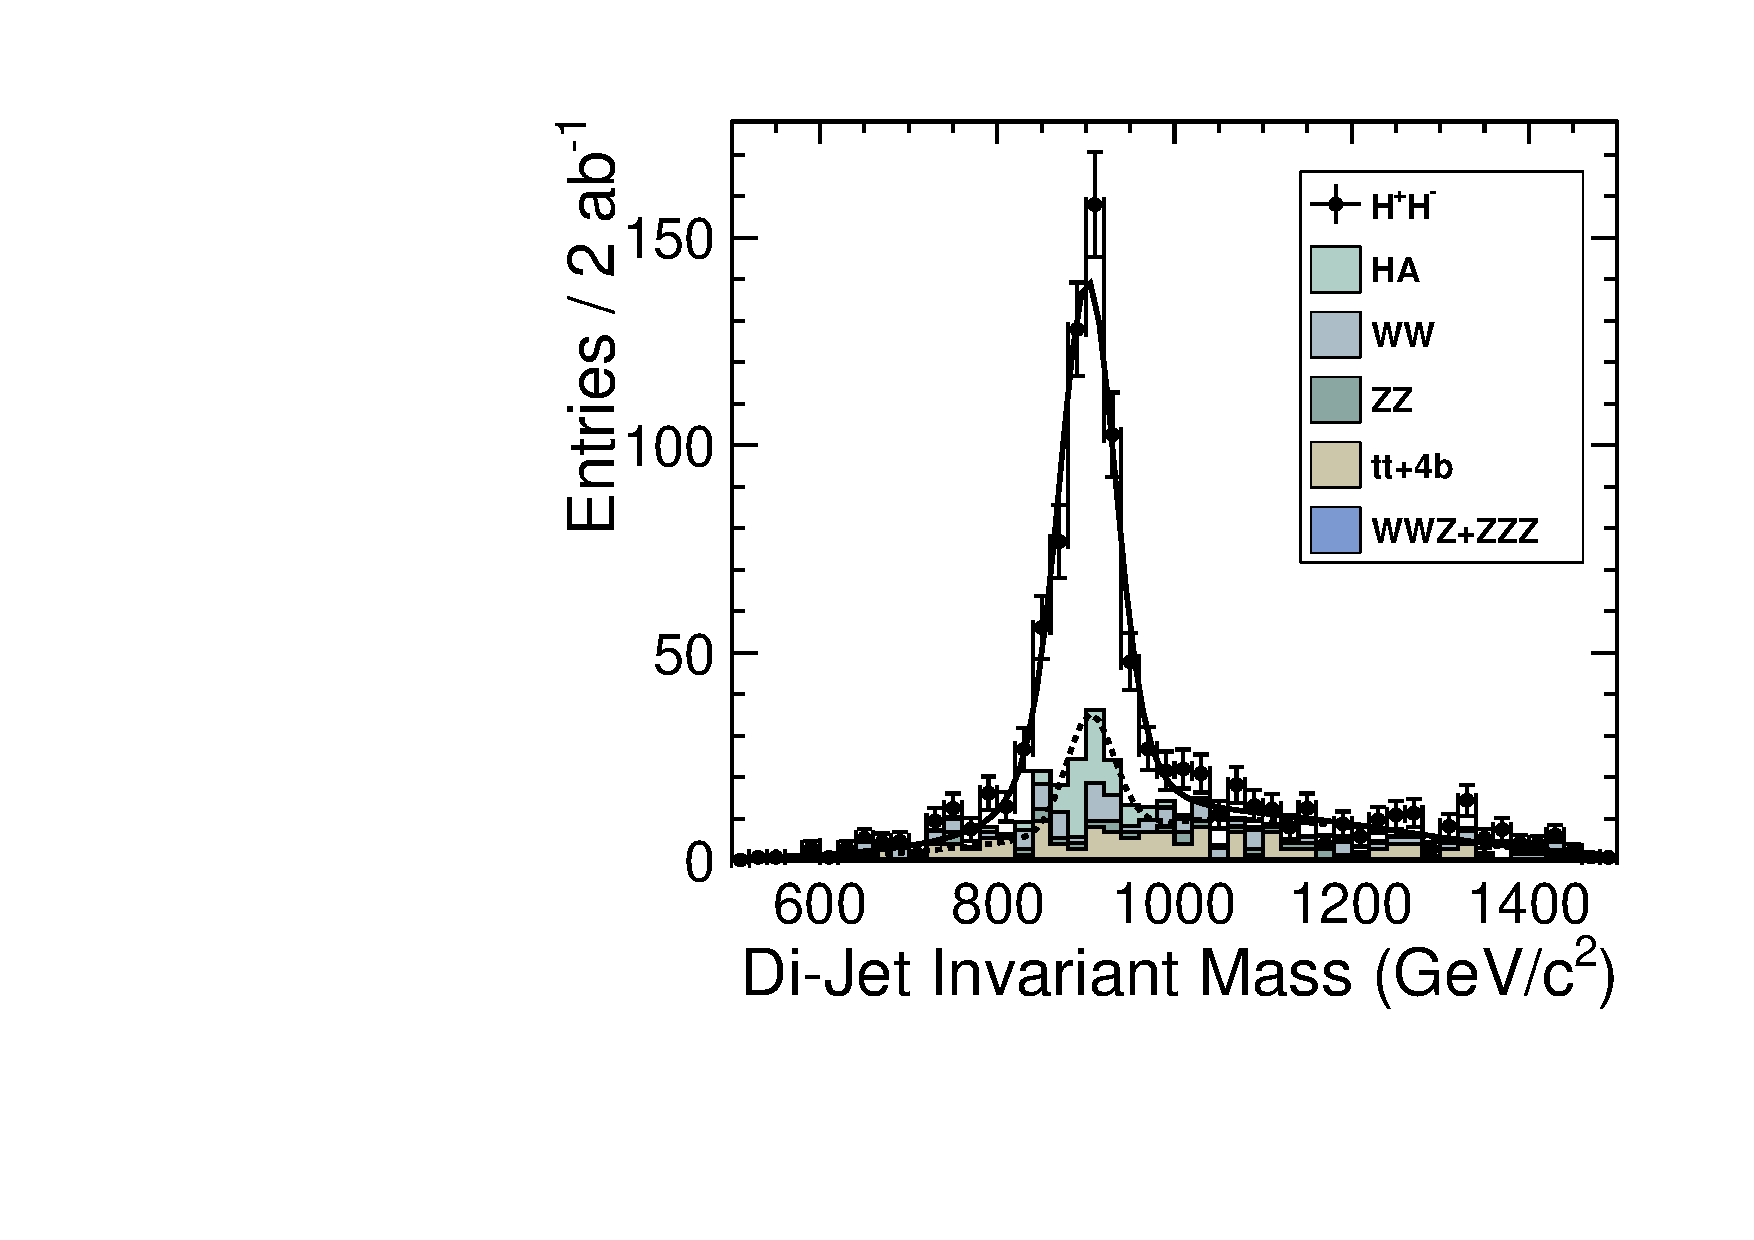
\includegraphics[width=4cm]{Hpm_Mass902_Bkg_CKFM_00BX_FJ.pdf}\\
{\scriptsize Statistical accuracy $\sigma(M)/M \sim0.3\%$.}\\
$\Rightarrow$ Evaluation of b-tagging and heavy jet reconstruction
\end{frame}

\begin{frame}
\frametitle{Squarks and Sleptons}
\begin{columns}[c]
\column{6cm}
\centering
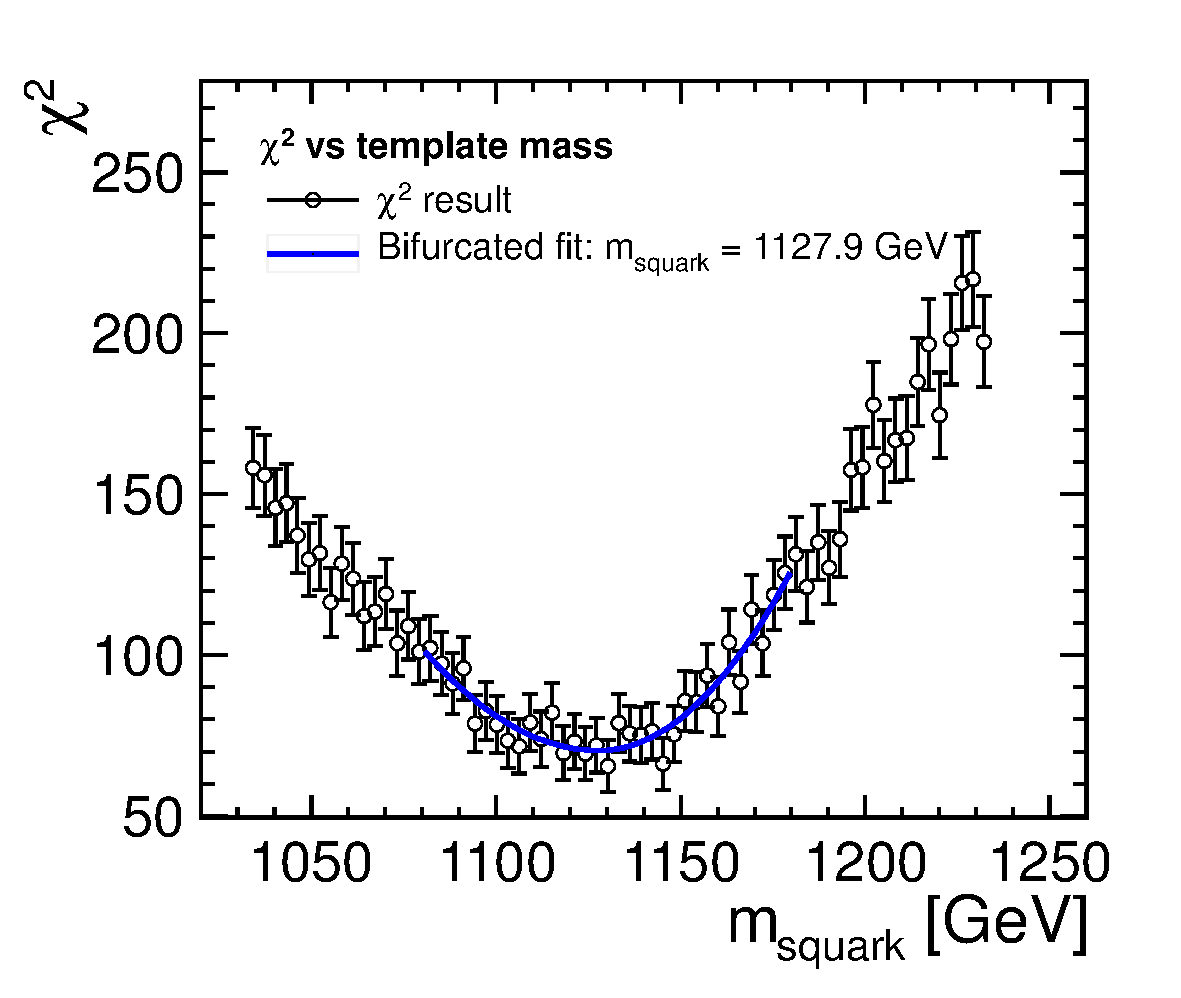
\includegraphics[width=5cm]{TemplateFit_Chi2SquarkMass.pdf}\\
\column{6cm}
\centering
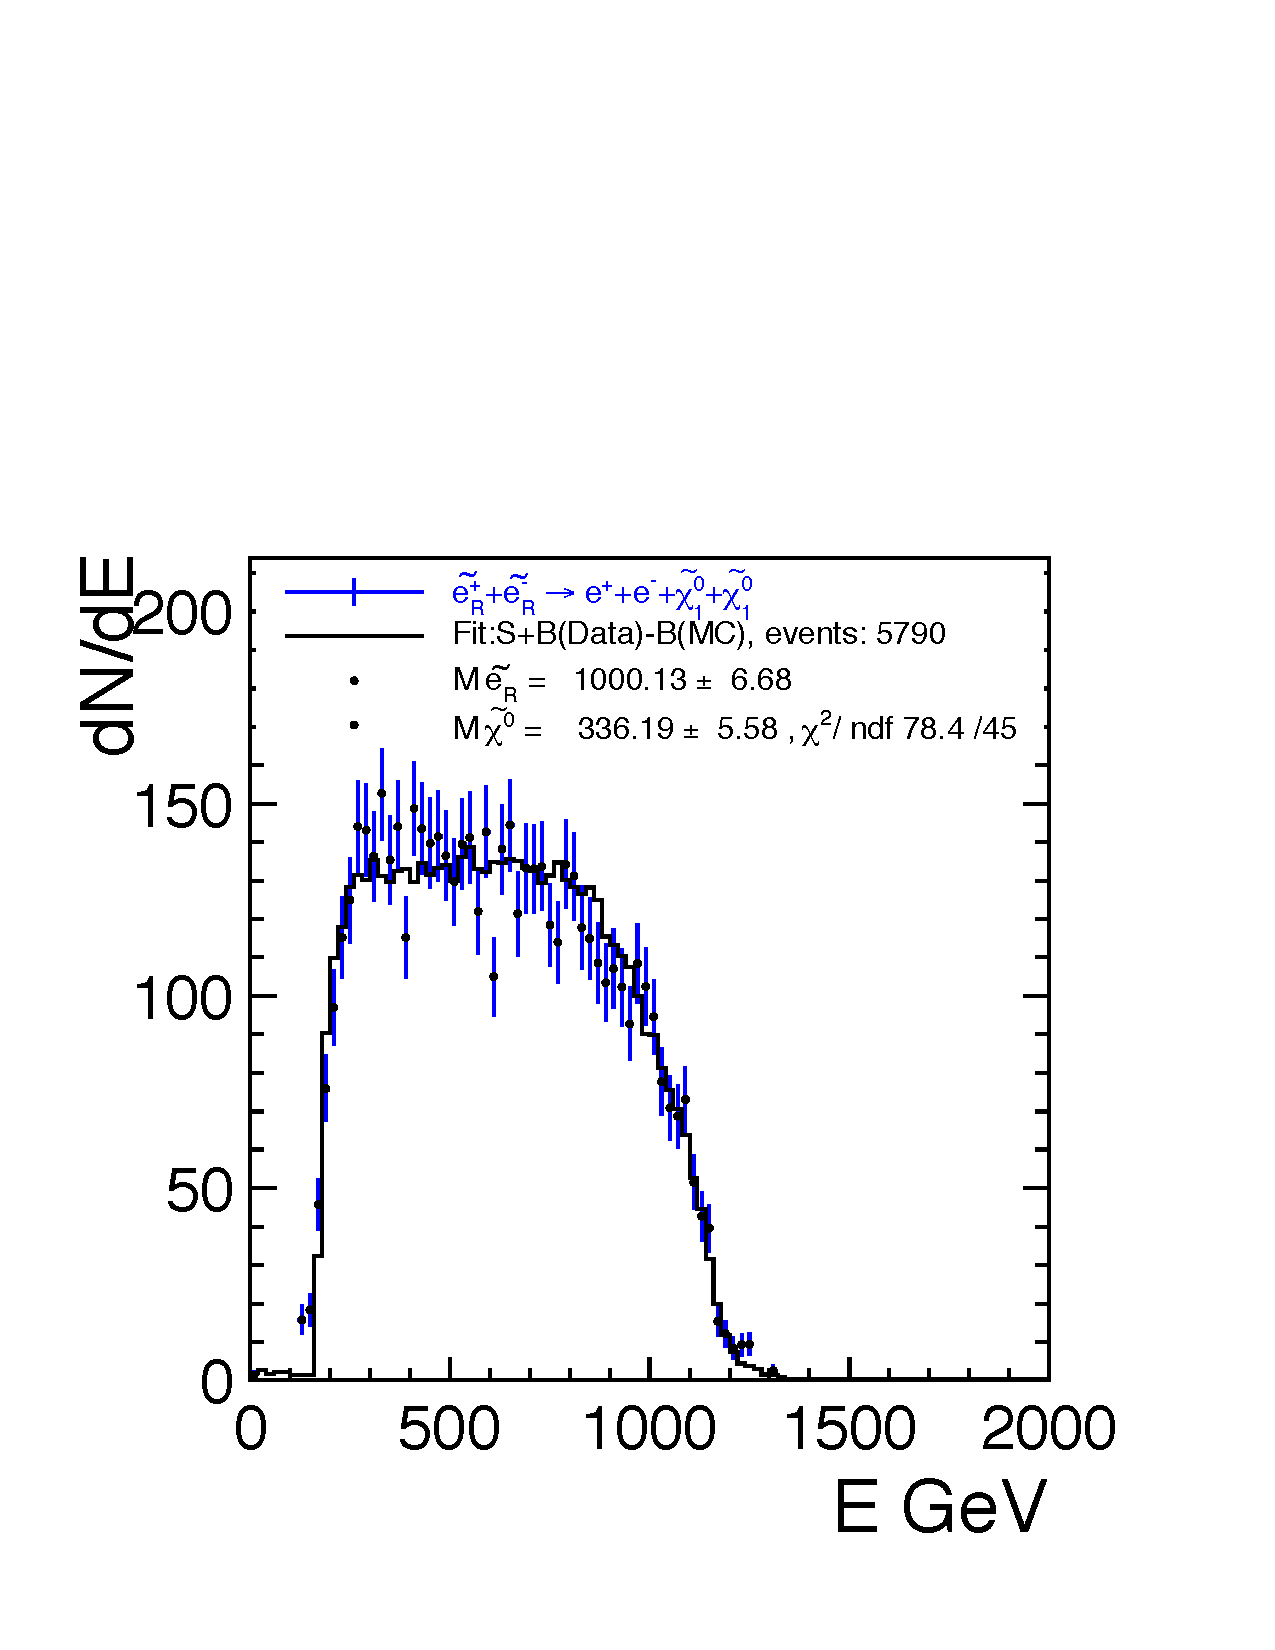
\includegraphics[width=5cm]{202_H1LPADC4.pdf}
\end{columns}
\begin{columns}[c]
\column{6cm}
\centering
$\sigma(m_{\PSq_{R}})/m_{\PSq_{R}}=0.5\%$
\column{6cm}
\centering
$\sigma(m_{\PSgm_{R}})/m_{\PSgm_{R}} = 0.6\%$\\
$\sigma(m_{\PSe_{R}})/m_{\PSe_{R}} = 0.3\%$\\
$\sigma(m_{\PSgxzi})/m_{\PSgxzi} = 1-2\%$
\end{columns}
~\\
$\Rightarrow$ Tests of jet reconstruction and Particle ID
\end{frame}
\begin{frame}
\frametitle{Top physics at 500GeV}
\begin{columns}[c]
\column{6cm}
\centering
Semi-leptonic decay:\\ 
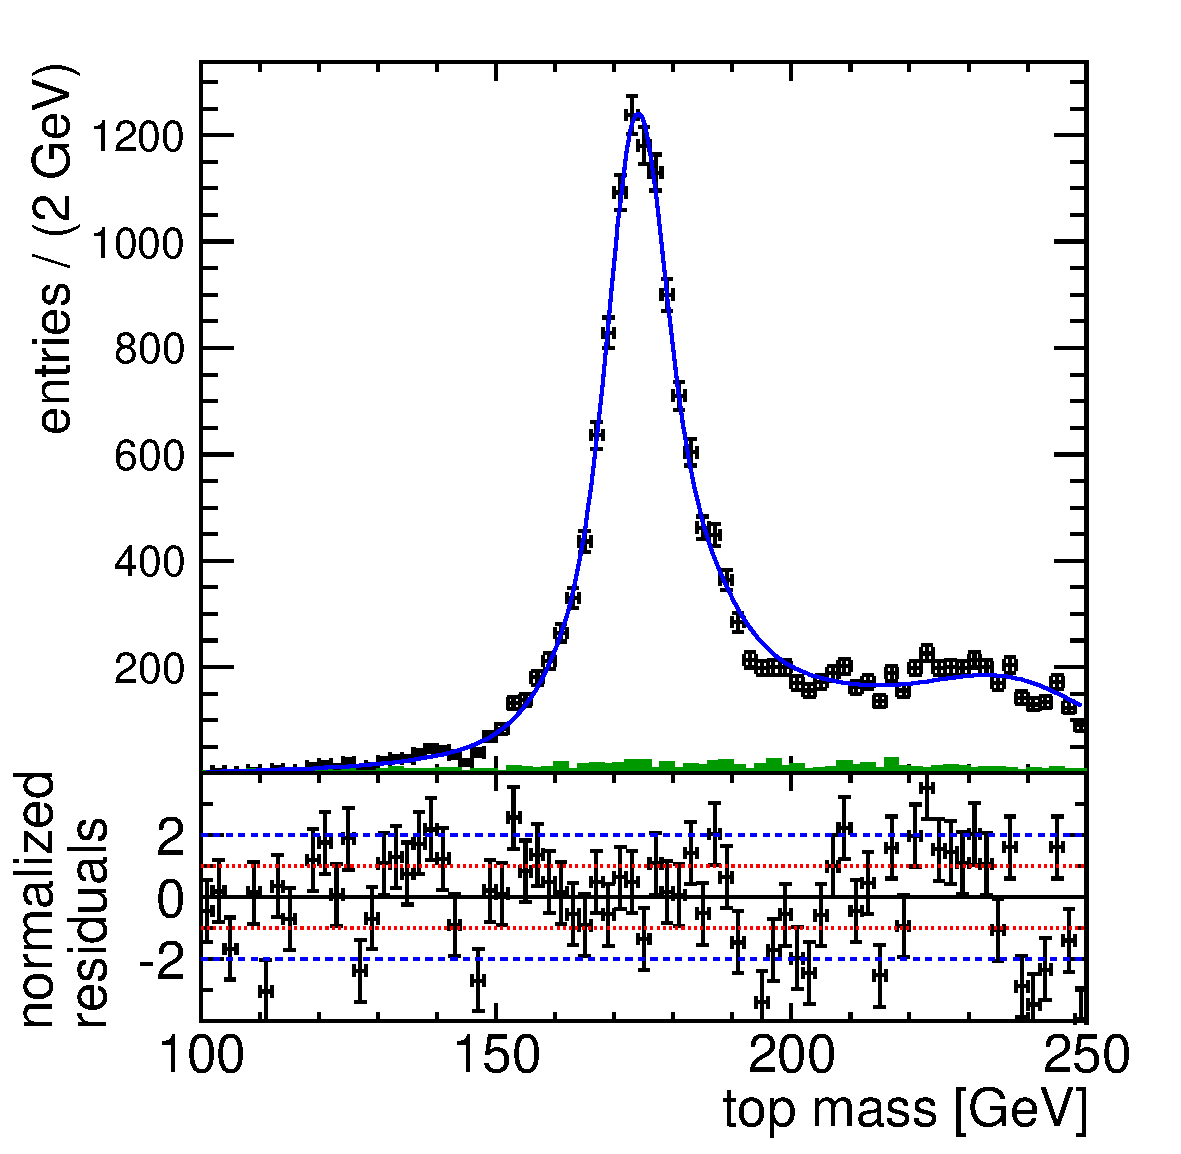
\includegraphics[width=5cm]{FinalFit-SemiLeptonic}\\
{\scriptsize
\begin{tabular}{c c }
\toprule
Top mass (GeV) & Top width (GeV)\\
\midrule
$174.28 \pm 0.09$ &  $1.55 \pm 0.26$
\end{tabular}}
\column{6cm}
\centering
Fully-hadronic decay:
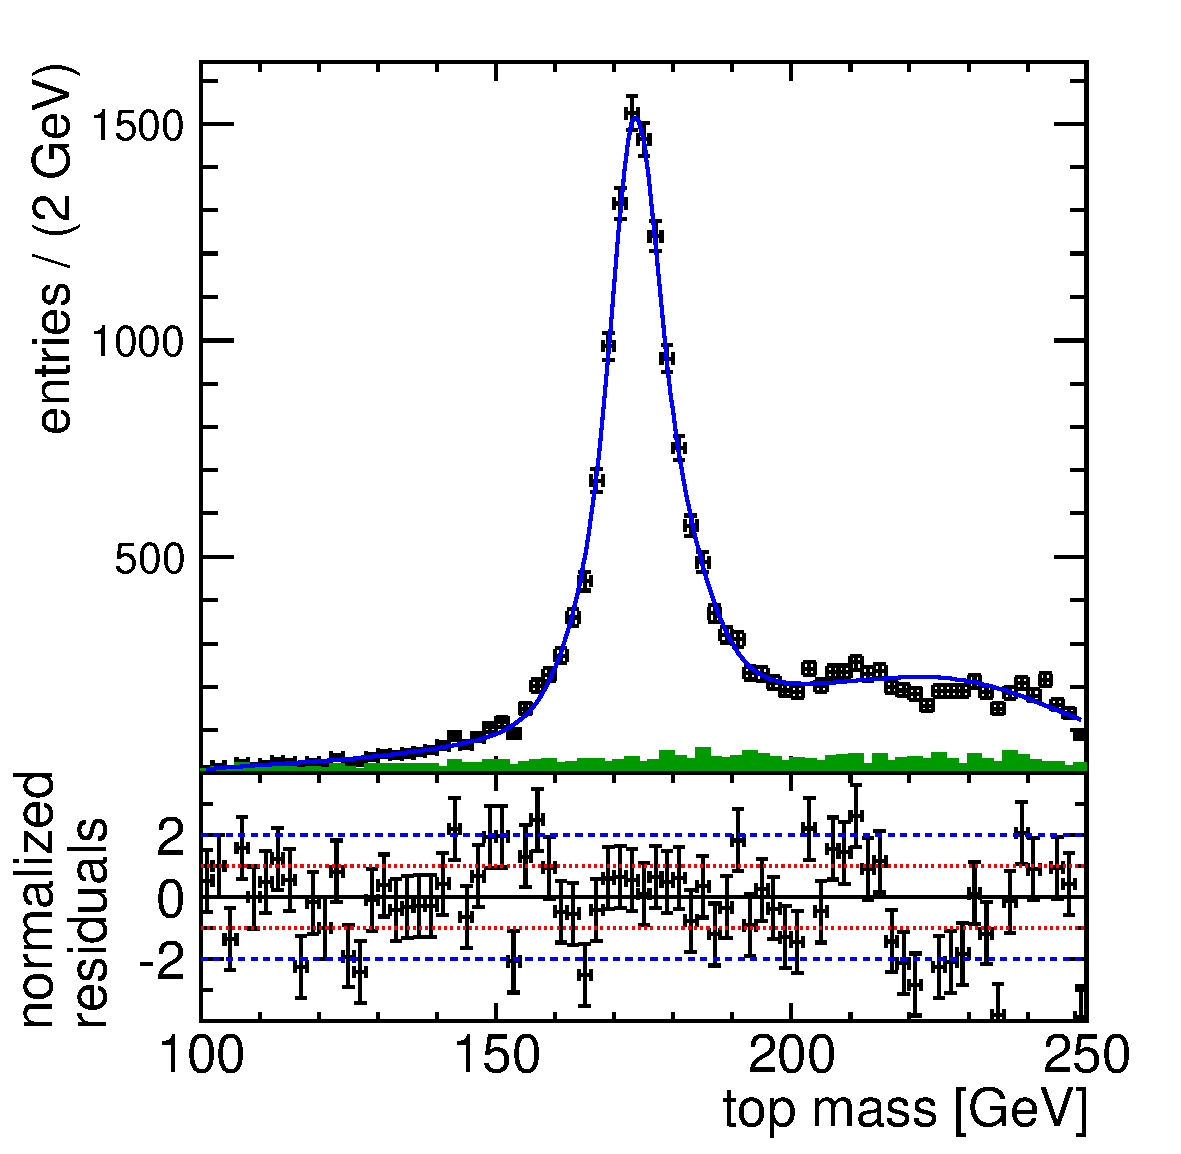
\includegraphics[width=5cm]{FinalFit-FullHadronic}\\
{\scriptsize
\begin{tabular}{c c }
\toprule
Top mass (GeV) & Top width (GeV)\\
\midrule
$174.07 \pm 0.08$ &  $1.33 \pm 0.22$
\end{tabular}}
\end{columns}
~\\
$\Rightarrow$ Compares well with ILC
\end{frame}

\end{document}